\documentclass{article}
\usepackage{graphicx} % Required for inserting images


\usepackage{graphicx}
\usepackage{amsmath,amsthm}
\usepackage{amssymb}
\usepackage{amsbsy}
\usepackage{amsfonts}
\usepackage[letterpaper,margin=0.6in]{geometry}
\usepackage{xypic}
\usepackage{hyperref}
\usepackage{multirow}
\usepackage{mathtools}
\usepackage{adjustbox}
\usepackage{bm}

\newcommand{\verteq}{\rotatebox{90}{$\,=$}}
\newcommand{\equalto}[2]{\underset{\scriptstyle\overset{\mkern4mu\verteq}{#2}}{#1}}


%\usepackage{ulem}
\usepackage{cancel}
\usepackage{lscape}
\usepackage{makecell}
%\usepackage[normalem]{ulem}
\usepackage{wasysym}
\usepackage{tikz}
\usepackage{tikz-cd}
\usepackage{stmaryrd}
\usepackage{mathrsfs}
\usetikzlibrary{arrows}


%\theoremstyle{theorem}
%\newtheorem{theorem}{Theorem}[section]

%\theoremstyle{lemma}
%\newtheorem{lemma}[theorem]{Lemma}
%\newtheorem{corollary}[theorem]{Corollary}
%\newtheorem{proposition}[theorem]{Proposition}


%\theoremstyle{definition}


\newtheoremstyle{mystyle}%                % Name
  {}%                                     % Space above
  {}%                                     % Space below
  {}%                                     % Body font
  {}%                                     % Indent amount
  {\bfseries}%                            % Theorem head font
  {.}%                                    % Punctuation after theorem head
  { }%                                    % Space after theorem head, ' ', or \newline
  {\thmname{#1}\thmnumber{ #2}\thmnote{ (#3)}}%                                     % Theorem head spec (can be left empty, meaning `normal')

\theoremstyle{mystyle}
\newtheorem*{definition}{Definition}%[section]
\newtheorem{theorem}{Theorem}%[section]
\newtheorem*{theorem*}{Theorem}
\newtheorem{corollary}[theorem]{Corollary}
\newtheorem*{corollary*}{Corollary}
\newtheorem{lemma}[theorem]{Lemma}
\newtheorem{proposition}[theorem]{Proposition}
\newtheorem*{example}{Example}
\theoremstyle{remark}
\newtheorem*{remark}{Remark}
\numberwithin{equation}{section}


\title{Bott Tu}

\author{Chunxiao Liu}

\begin{document}

\maketitle




\tableofcontents

\section{Differential Forms in Algebraic Topology}

\begin{itemize}
\item Lectures: \url{https://www.youtube.com/watch?v=96Nr-Aba3iI&list=PLQZfZKhc0kiA149d8nmkY7DARwyjzHfl0&ab_channel=NCTSMathDivision}

\item Book: \emph{Differential Forms in Algebraic Topology} by Loring W. Tu and Raoul Bott.
\end{itemize}


\subsection{Lecture 1: De Rham Complex on $\mathbb{R}^n$}

Def: a $k$-tensor on a vectpr space $V$ is a $k$-linear function $\alpha \colon V\times\cdots \times V\rightarrow \mathbb{R}$; a $k$-tensor is \emph{alternating} if $\alpha(v_{\sigma(1)},...,v_{\sigma(k)}) = (-1)^{\mathrm{sgn}(\sigma)}
\alpha(v_1,...,v_k)$; Denote $A_k(V):= \{\text{alternating }k\text{-tensors}\}$. 

Open subset $U$; tangent space $T_p(U)$;

Def: A $k$-form on $U$ is an assignment to each $p\in U$ of an alternating $k$-tensor $\omega_p\colon T_pU\times \cdots \times T_pU\rightarrow \mathbb{R}$. I.e., a $k$-form is a funtion $\omega \colon U\rightarrow \amalg_{p\in U} A_k(T_pU)$, s.t. $\omega_p \in A_k(T_pU)$. 

Def: let $C^\infty(U) :=\{C^\infty \text{ func }f\colon U\rightarrow \mathbb{R}\}$. One form: For $f \in C^\infty$, define $df$ to be the 1-form s.t. $\forall v \in T_pU$, $(df)_p\colon T_pU\rightarrow \mathbb{R}$ s.t. $\forall v \in T_pU$, $(df)_p(v) = D_vf$, the directional derivative along $v$.  

Usually $v_p =  v^i e_{i,p}$; $D_vf =  v^i \partial_{x^i}|_p f$, this means it is the handy to make the (formal) identification that $e_{i,p} = \frac{\partial}{\partial x^i}|_p$, i.e. denote the basis of the vector as $\frac{\partial}{\partial x^i}$. 

Then: what is $dx^i$? it is a 1-tensor: $(dx^i)_p\colon T_pU\rightarrow \mathbb{R}$, $(dx^i)_p(v) = D_v(x^i)= v_i$. So: $d x^i$ is the 1-form on $U$ that picks out the $i$th component of a vector $v \in T_pU$ at all $p \in U$. 

Def: The wedge product. If $\alpha \in A_o(V)$ and $\beta \in A_l(V)$, then $\alpha \wedge \beta \in A_{k+l}(V)$, defined by $(\alpha \wedge \beta)(v_1,...,v_{k+l}) = \frac{1}{k!l!}\sum_{\sigma \in S_{k+l}}
\mathrm{sgn}(\sigma) \alpha(v_{\sigma(1)},...,v_{\sigma(k)})
\beta(v_{\sigma{k+1}},...,\sigma_{\sigma(k+l)})$. 

Def: If $\alpha$ is a $k$-form and $\beta$ an $l$-form on $U$, then $(\alpha\wedge \beta)_p := \alpha_p\wedge \beta_p$, $\forall p\in U$.

Differential forms in terms of coordinates:

Def: dual space. If $V$ is a vector space, then the dual space $V^\vee:=\{\text{linear functions }f\colon V\rightarrow \mathbb{R}\}$.

Prop: $\{(d x^1)_p,...,(d x^n)_p\}$ is the dual basis for $(T_pU)^\vee$ to $\{\partial_{x^1}|_p,...,\partial_{x^n}|_p\}$. (Proof: the meaning of $d x^i$ and $\partial_{x^i}$ has been clarified above, so we have $(dx^i)_p(\partial_{x^j}|_p) = \delta^i_j$. )

Def. $A$ 1-form $\omega = a_i d x^i$ on $U$ is smooth, or $C^\infty$, if fall $a_i$ are $C^\infty$ functions.

Theorem. (Multilinear Algebra) If $\alpha^1,...,\alpha^n$ is a basis for 1tensors on $V$, then $\{\alpha^{i_1}\wedge \cdots \wedge \alpha^{i_k},i_1<\cdots <i_k\}$ is a basis for $k$-tensors on $V$.

Theorem. Every $k$-form $\omega$ on $U$ can be written uniquely as $\omega \in \sum_{1\leq i_1<\cdots <i_k\leq n} a_{i_1...i_k} d x^{i_1}\wedge \cdots \wedge d x^{i_k} \equiv \sum_I a_I d x^I$, where $I = (i_1,...,i_k)$ with $1\leq i_1\cdots <i_k\leq n$. 

Def. A $k$-form $\omega = a_I d x^I$ is $C^\infty$ if all $a_I$ are $C^\infty$ functions on $U$. 

Notation: $\Omega^k(U) = \{C^\infty~ k\text{-forms on }U\}$. 

Theorem. There exists a unique $\mathbb{R}$-linear map $d\colon \Omega^*(U)\rightarrow \Omega^{*+1}(U)$, s.t. (1) $d$ is an antiderivation (defined as $d(\omega \wedge \tau) = d\omega \wedge \tau + (-1)^{\mathrm{deg}(\omega)} \omega \wedge d\tau$); (2) $d\cdot d = 0$, and (3) $d\colon \Omega^0(U)\rightarrow \Omega^1(U)$ is the differential of a function. (It's simple to prove that $\Omega^0(U) = C^\infty (U)$.)


Therefore, there exists a sequence

$$\Omega^0(U)\xrightarrow{d^0}\Omega^1(U)\xrightarrow{d^1}\cdots \xrightarrow{d^{n-1}} \Omega^n(U)\rightarrow 0,$$
called the de Rham complex (a complex is a sequence of vector spaces where the adjacent maps compose to zero).

As $d^k\circ d^{k+1}=0$, $\mathrm{im} d^{k-1}\subset \mathrm{ker} d^k d^k$, so we can define:

Def: the de Rhan cohomology is defined as $H^k(U) = \mathrm{ker}d^k/\mathrm{im} d^{k-1}:= Z^k(U)/B^k(U)$. 

Example: calculate $H^*(\mathbb{R})$. $0\rightarrow \Omega^0(\mathbb{R})\xrightarrow {d^0}\Omega^1(\mathbb{R})\rightarrow 0$, where $\Omega^0(\mathbb{R}) = C^\infty(\mathbb{R})$, and $\Omega^1(\mathbb{R}) = \{g(x)dx|g\in C^\infty(\mathbb{R})\}$. 

$Z^0(\mathbb{R}) = \{f \in C^\infty(\mathbb{R})|df=0\}$, since $df=f'(x)dx=0$ so $f'(x)=0$, so $f$ is constant, so $\mathbb{Z}^0(\mathbb{R}) = \mathbb{R}$; $B^0(\mathbb{R})=0$, so $H^0(\mathbb{R}) = \mathbb{R}$. Then, $Z^1(\mathbb{R}) = \{g(x)dx\} \simeq C^\infty(\mathbb{R})$; $B^1(\mathbb{R}) = \{df=f'(x)dx|f\in C^\infty(U)\}$, since any $C^\infty$ function is the derivative of some $C^\infty$ function, so $Z^1=B^1$, $H^1(\mathbb{R})=0$. 


\subsection{Lecture 2: Compact supports, manifolds}

Def: A $k$-form $\omega$ is \emph{closed} if $d\omega=0$; $\omega$ is \emph{exact} if $\omega = d\tau$ for some $\tau\in \Omega^{k-1}(U)$. 

Compact support:

Def. The \emph{zero set} of a $k$-form $\omega$ on $U$ (an open set of $\mathbb{R}^n$) is $Z(\omega) =\{p\in U|\omega_p = 0\}$; The \emph{support} of $\omega$ is $\mathrm{supp}(\omega) = \text{Closure}_U(U\backslash Z(\omega))$. 

Def $\Omega^k_c(U) := \{C^\infty~k \text{-forms with compact support in }U\}$. 

Proposition. $d$ is support-decreasing: for $\omega \in \Omega^k(U)$, $\mathrm{supp}(d\omega)\subset \mathrm{supp}(\omega)$. (Let $p\in \text{supp}(\omega)^c$. since the support is closed by definition, there exists a neighborhood $V$ of $p$ s.t. $V \subset (\text{supp}\omega)^c$. Therefore $\omega \equiv 0$ on $V$. Hence $d\omega \equiv 0$ on $V$, so $p \notin \text{supp}(d\omega)$.)

Corollary. If $\omega\in \Omega^k(U)$, has compact support, so does $d\omega$. (Use the knowledge from point set topology that a closed subset of a compact set is compact.)

So can talk about 

$$\Omega^0_c(U)\xrightarrow{d^0}\Omega^1_c(U)\xrightarrow{d^1}\cdots \xrightarrow{d^{n-1}} \Omega^n_c(U)\rightarrow 0,$$

Def: the de Rham cohomology with compact support is defined as $H^k_c(U) := Z^k_c(U)/B^k_c(U)$. 

Def A $0$-th tensor on $V$ is a constant, $A_0(V) = \mathbb{R}$. Thus $\Omega^0(U) = \{C^\infty~0\text{-forms on }U\} = C^\infty(U)$.

Example: calculate $H^*_c(\mathbb{R})$. $0\rightarrow \Omega^0_c(\mathbb{R})\xrightarrow {d^0}\Omega^1_c(\mathbb{R})\rightarrow 0$, where $\Omega^0_c(\mathbb{R}) = C^\infty_c(\mathbb{R})$

$Z^0_c(\mathbb{R}) = \{f \in C^\infty_c(\mathbb{R})|df=f'(x)dx = 0\}$, so $f'(x)=0$ and $f$ is a constant function that's equal to zero, so $Z^0_c(\mathbb{R}) = 0$, and $H^0_c(\mathbb{R}) = 0$. 

$Z^1_c(\mathbb{R}) = \{g(x)dx = g\in C^\infty_c(\mathbb{R}),dg=0\} = \{g(x)dx\}$, $B^1_c(\mathbb{R}) = \{f'(x)dx |f \in C^\infty_c (\mathbb{R})\}$. If $g(x)=f'(x)$, then $\int^\infty_{-\infty} g(x)dx=0$. Then: suppose $\int^\infty_{-\infty} g(x)dx=0$, find $f(x)$ with compact support s.t. $g(x)=f'(x)$. $f(x)=\int^x_{-\infty}g(u)du$. 
(Then: prove that $\mathrm{ker}\int^\infty_{-\infty} = B^1_c(\mathbb{R})$, and by 1st isomorphism of linear algebra, we have $Z^1(\mathbb{R})/\mathrm{ker}\int^\infty_{-\infty} = \mathrm{im}\int^\infty_{-\infty} = \mathbb{R}$.)

To summarize: $H^*(\mathbb{R}) = \left\{\begin{array}{ll} \mathbb{R} & deg ~0\\0 & deg ~1\end{array}\right.$, $H^*_c(\mathbb{R}) = \left\{\begin{array}{ll} 0 & deg ~0\\\mathbb{R} & deg ~1\end{array}\right.$
We already noticed some ``duality''. This will eventually become the Poincar\'e duality.




\begin{definition}[Manifold] A \emph{topological manifold (or manifold for short)} is a locally Euclidean (for all $p\in M$, $\exists$ a neighborhood $U$ and a homeomorphism $\phi\colon U\rightarrow \phi(U) \subset \mathbb{R}^n$; chat $=(U,\phi)$, charts $(U,\phi)$ and $(V,\psi)$ are $C^\infty$-compatible iff $\phi\circ \psi^{-1}\colon \psi(U\cap V) \rightarrow \phi(U\cap V)$, and $\psi\circ \phi^{-1}\colon \phi(U\cap V)\rightarrow \psi(U\cap V)$ are $C^\infty$; an atlas is $\{(U,\phi)\}$, i.e. a collection of $C^\infty$-compatible charts that cover $M$); Hausdorff, 2nd countable, topological space $M$.
\end{definition}

\textcolor{red}{[Intuitive understanding of manifolds: \emph{``(1) transition function has to be $C^\infty$; (2) Haussdorf: can separate points with open sets. this tells that we must have enough open sets to separate points, i.e. the topology cannot be too small; (3) 2nd countable: must have a basis that's countable; it means that the topology is not too big. For manifolds: the topology is not too big and not too small!''}]}

Def. A $C^\infty$ manifold is a topological manifold $M$ together with a maximal atlas.

Def: Tangent space: $T_pM=$ vector space spanned by $\partial_{x^1}|_p$, ..., $\partial_{x^n}|p$. 


Def: A $k$-form on a manifold is an asignment to each point $p$ of the manifold, an alternating $k$-tensor on the tangent space at $p$.

Then, we can define $H^k(M)$, and $H^k_c(M)$. 

\subsection{Lecture 3: Diffeomorphism invariance, exat sequences}

Pullback under $C^\infty$ map: $\psi\circ F\circ \phi^{-1}$ is $C^\infty$ map.

The pullback $F^*\colon \Omega^k(M)\rightarrow \Omega^k(N)$ is defined  so that (1) for $g \in \Omega^0(M)$, $F^*(g) = g\circ F$; (2) $F^*$ commutes with $+$, $\cdot$, $\wedge$, $d$; (3) $(F\circ G)^* = G^*\circ F^*$. 

If $\omega \in \Omega^k(M)$, then on a chart $(V,y^1,...,y^n)$, $\omega = \sum a_I dy^I$, $F^*\omega = (F^*a_I) (d F^* y^I)
=(a_I\circ F) d F^I$. 

Pullback in cohomology: 

Proposition: $F^*$ takes closed forms to closed forms and exact forms to exact forms.

In principle we write the induced map on cohomology as $F^\#$; but we'll also use $F^*$ in place of $F^\#$.

Theorem: A diffeomorphism $F\colon N\rightarrow M$ induces an isomorphism $F^*\colon H^*(M)\rightarrow H^*(N)$. 

The pullback of $\omega \in \Omega^k_c(M)$ need not have compact support. (must have compact support if it is deffeomorphism.)

Exact sequences of vector spaces

Exact sequences of cochain complexes:

Def: a cochain complex (differential complex) is a sequence of vector spaces and linear maps $C\colon \cdots \rightarrow C^{k-1}\xrightarrow{d_{i-1}} C^k\xrightarrow{d_k} C^{k_1}\rightarrow \cdots$ s.t. $d_k\circ d_{k-1} = 0$ $\forall k \in \mathbb{Z}$ (so that $\mathrm{im}d_{k-1}\subset \mathrm{ker} d_k$).

Def: $H^k(C) = \frac{\mathrm{ker}d_k}{\mathrm{im}d_{k-1}}$. 

Def: a cochain map $\varphi\colon A\rightarrow B$ is a collection $\varphi_k\colon A^k\rightarrow B^k$ of linear maps s.t. $\varphi_{k+1}\circ d_k  = d'_k\circ \varphi$ $\forall k$, i.e. it makes the following diagram commutative:
$$
\begin{tikzcd}
\cdots \ar[r] & A^{k-1} \ar[r,"d_{k-1}"] \ar[d,"\varphi_{k-1}"] & A^k \ar[r,"d_k"]\ar[d,"\varphi_k"] & A^{k+1} \ar[r]\ar[d,"\varphi_{k+1}"] & \cdots \\
\cdots \ar[r] & B^{k-1} \ar[r,"d'_{k-1}"]  & B^k \ar[r,"d'_k"]& B^{k+1} \ar[r] & \cdots \\
\end{tikzcd}
$$
\textcolor{red}{[In later lectures quite often we will need to show the existence of a cochain map $\varphi$. Then the essence is to show that we have a commutative relation $d \varphi = \varphi d$.]}

Def: $Z^k(C) = \{c\in C^k|dc = 0\}$, $B^k(C) = \{c\in C^k| c=dc' \text{ for some }c' \in C^{k-1}\}$.


A cochain map $\varphi\colon A\rightarrow B$ induces a linear map $\varphi^*\colon H^*(A)\rightarrow H^*(B)$. 

Def: A short exact sequence of cochain complexes: $0\rightarrow A\xrightarrow{i} B\xrightarrow{j} C\rightarrow 0$ where $i$, $j$ are cochain maps, is a sequence of linear maps s.t. $\forall k\in \mathbb{Z}$,
$0\rightarrow A^k\xrightarrow{i}B^k\xrightarrow{j} C^k\rightarrow 0$ is a short exact sequence of vector spaces. 

In the next lecture we will show that a short exact sequence of cochain complexes $0\rightarrow A\xrightarrow{i} B\xrightarrow{j} C\rightarrow 0$ induces 
a long exact sequence in cohomology: $\cdots \rightarrow H^k(A)\xrightarrow{i^*}H^k(B)\xrightarrow{j^*}H^k(C)\xrightarrow{d^*}
H^{k+1}(A)\rightarrow \cdots$.






\subsection{Lecture 4: Zig-Zag Lemma, Mayer--Vietoris Sequence}


\begin{theorem*}[Zig-zag lemma] An exact sequence of cochain complex and cochain maps 
$$0\rightarrow A\xrightarrow{i}B\xrightarrow{j} C\rightarrow 0$$
induces a long exact sequence
$$\cdots \rightarrow H^k(A)\xrightarrow{i^*}H^k(B)\xrightarrow{j^*}H^k(C)\xrightarrow{d^*}
H^{k+1}(A)\rightarrow \cdots$$
\end{theorem*}

Constructing the connecting homomorphism:
$$
\begin{tikzcd}
(k+2)\text{th row}   & 0&&\\
(k+1)\text{th row}   & a\rar[mapsto,"i"]\ar[u,"d"] &db\ar[r,"j"]&0\\
k\text{th row}& &b\ar[r,"j"]\ar[u,"d"]& c\ar[u,"d"]
\end{tikzcd}
$$ 

Step: start with $[c]\in H^k(\mathcal{C})$, we have $dc=0$. Also, because $0\rightarrow A\xrightarrow{i} B\xrightarrow{j}C\rightarrow 0$ is exact, so $j\colon B^k\rightarrow C^k$ is onto, so there exists $b\in B^k$ s.t. $b\xrightarrow{j} c \xrightarrow{d}0$. Also, we have $b\rightarrow db$ which belongs to $B^k\xrightarrow{d} B^{k+1}$. Note that $jdb=0 \in C^{k+1}$ due to the commutative square of $B^{k+1},C^{k+1}$, $B^k$ and $C^k$. Then $db \in \mathrm{ker}(j\colon B^{k+1}\rightarrow C^{k+1}$ so there $\exists$ $a \in A^{k+1}$ s.t. $ia = db$. Note that $a \in A^{k+1}$ is unique as $i$ is injective. Finally, we need to show that $da = 0$: this is true as $ida = d(ia) = d(db) = 0$, and that $i$ is injective. (Now: this construction made a choice on $b$ and $c$; needs to show that $d^*[c]$ is independent of these choices. Omit here.)

Here, the essence is the chasing along $\begin{tikzcd}[column sep = small, row sep = small]a \ar[r,"i"]&db&\\&b\ar[r,"j"]\ar[u,"d"]&c\end{tikzcd}$. 

Def: $C^\infty$ partition of unity: A $C^\infty$ of $1$ on a $C^\infty$ manifold $M$ is a collection $\{\rho_\alpha\colon M\rightarrow \mathbb{R}\}_{\alpha \in A}$ of $C^\infty$, s.t. (1) every $p\in M$ has a neighborhood on which $\sum_{\alpha \in A}\rho_\alpha$ is a finite sum; (2) $\sum_{\alpha \in A}\rho_\alpha = 1$. 

Theorem: given an open cover $\{U_\alpha\}_{\alpha \in A}$ of a $C^\infty$ manifold $M$, there exists a $C^\infty$ partition of unity, $\{\rho_\alpha\}_{\alpha \in A}$, subordinate to $\{U_\alpha\}_{\alpha \in A}$. (Such a nice property exists for $C^\infty$ and continuous function; but for complex manifolds there's no such property, making their study more challenging.)

\begin{theorem*}[Mayer--Vietoris Sequence]
Let $\{U,V\}$ be an open cover of a manifold $M$, i.e. $M=U\cup V$. We will show that the following short exact sequence holds:
\begin{equation}
0\rightarrow \Omega^k(M)\xrightarrow{i} \Omega^k(U)\oplus \Omega^k(V)\xrightarrow{j} \Omega^k(U\cap V)\rightarrow 0,
\end{equation}
where $i(\omega) = (\omega|_U,\omega|_V)$ is restriction, and $j(\omega|_U,\omega|_V) = \omega_V|_{U\cap V} - \omega_U|_{U\cap V}$ is difference.
\end{theorem*}

\noindent Proof: see the book P22.

Cohomology of disjoint union: If $M = A\amalg B$ (disjoint union), then $H^k(M) = H^k(A)\oplus H^k(B)$. 

Cohomology in degree 0: If $M$ has $m$ connected components, then $H^0(M) = Z^0(M) = \mathbb{R}^m$.

Cohomology of $S^1$: $H^{0,1}(S^1)=\mathbb{R}$ (other degree vanishes).



\subsection{Lecture 5: Homotopy invariance}

Homotopy: let $N$, $M$ be smooth manifolds. $N\times[0,1]$ is a manifold with boundary.

Def: $F\colon N\times[0,1]\rightarrow M$ is \emph{smooth} if can be extended to a smooth map on a neighborhood of $N\times[0,1]$ in $N\times \mathbb{R}$.

Def: $f_0,f_1\colon N\rightarrow M$ are \emph{smoothly homotopic}, denoted as $f_0\sim f_1$, if $\exists$ a $C^\infty$ map $F\times N\times [0,1]\rightarrow M$, s.t. $F(x,0)=f_0(x)$, $F(x,1)=f_1(x)$. (E.g.: straight-line homotopy.)

Def. $f\colon N\rightarrow M$ is a \emph{homotopy equivalence} if $\exists$ $g\colon M\rightarrow N$ s.t. $g\circ f\sim 1_N$ and $f\circ g\sim 1_M$. $g$ is a \emph{homotopy inverse} of $f$, and in this case, $M$ and $N$ are \emph{homotopy equivalent}, or have the same \emph{homotopy type}. A manifold with the homotopy type of a point is \emph{contractible}.

Example: $r\colon \mathbb{R}^2\backslash\{0\} \rightarrow ^1$, $r(x) = x/||x||$ is a homotopy equivalence (define $i\colon S^1\rightarrow \mathbb{R}^2\backslash\{0\}$ the inclusion; show $r\circ i=1_{S^1}$ and $i\colon r$ homotopic to $1_{\mathbb{R}^2\backslash\{0\}}$.), so they have the same homotopy type.

Def. Let $A\subset M$. A map $r\colon M\rightarrow A$ is a \emph{retraction}, if $r|_A = 1_A$ (or $r\circ i=1_A$). A retraction is a \emph{deformation retraction} if $i\circ r\sim 1_M$.

Proposition: A deformation retraction $r\colon M\rightarrow A$ is a homotopy equivalence.

Homotopy Axiom (see e.g. Steenrod, first a theorem, then used as an axion to define cohomology theories): it roughly says that homotopy maps induce the same maps in cohomology. 

\begin{theorem*}[Homotopy axiom]
If $f\colon N\rightarrow M$ is a $C^\infty$ map of manifolds, then we have $f^*\colon \Omega^k(M)\rightarrow \Omega^k(N)$, $\omega\mapsto f^*(\omega)$, and $f^\#\colon H^*(M)\rightarrow H^*(N)$, $f^\#([\omega])=[f^*(\omega)]$ (also very often written just as $f^*$). Theorem: if $f\sim g$, then $f^\#\sim g^\#$. 
\end{theorem*}


\begin{corollary*} If $f\colon N\rightarrow M$ is a homotopy equivalence, then $f^*\colon H^*(M)\rightarrow H^*(N)$ is an isomorphism.
\end{corollary*}


(A vector space that's also a ring is an \emph{algebra}. Cohmology preserves addition, scalar multiplication and wedge product, so the isomorphism is in the sense of isomorphism of algebras.)

Proof: let $g\colon M\rightarrow N$ be a homotopic inverse of $F$, then $(g\circ f)^*=1_{H^*(M)}$ and $(f\circ g)^* = 1_{H^*(M)}$, then $f^*\colon H^*(M)\rightarrow H^*(N)$ is bijective, hence n algebra isomorphism.

Corolary: if $M$ and $N$ have the same homotopy type, then $H^*(M)\simeq H^*(N)$.

Example: $H^*(S^1\times [0,1]) \simeq H^*(\mathbb{R}^2\backslash\{0\})\simeq H^*(S^1) =\mathbb{R}$ in degree 0,1, an vanishes in other degrees.

Example: $H^*(\mathbb{R}^n) = H^*(pt) = \mathbb{R}$ in deg 0 but 0 in deg$>0$.

(Generators of $H^0(S^1)$ is any nonzero constant function; Generators of $H^1(S^1)$ is a 1-form that's non-exact: if $\omega = d\tau$ an exact 1-form on $S^1$, then $\int_{S^1}\omega = \int_{S^1}d\tau=0$ by Stoke's theorem, so any generator is represented a 1-form whose integral is not zero, e.g. $d\theta \in \Omega^1(S^1)$. Usually we take $[\frac{1}{2\pi}d\theta] \in H^1(S^1)=\mathbb{R}$ as the preferred generator.)

Example: Integral on a cylinder: suppose $\omega \in \Omega^1(C)$ is a closed form. Claim: $\int_{S_A}\omega = \int_{S_B}\omega$, where $S_A$, $S_B$ are the upper and lower boundaries of a cylinder $C$ with a given orientation. (Proof: $0=\int_Cd\omega = \int_{\partial C} \omega$, by Stoke's theorem.

Example: Cohomology of a torus: use Mayer--Vietoris to decompose the torus $M$ to two cylinders $U$ and $V$, then we have the LES with easy entries $0\rightarrow H^0(M)=\mathbb{R}\xrightarrow {i_0^*}\mathbb{R}\oplus \mathbb{R}\xrightarrow{j_0^*}\mathbb{R}\oplus \mathbb{R}\xrightarrow{d_0^*} H^1(M)\xrightarrow {i_1^*}\mathbb{R}\oplus \mathbb{R}\xrightarrow {j_1^*} \mathbb{R}\oplus \mathbb{R} \xrightarrow{d_1^*} H^2(M)\rightarrow 0$. Next, need to characterize the map $j_1^*$: Let $[\omega_U]\in H^1(U)$ be the preferred generator, then $1 = \int_{S_U} = \int_{S_A}\omega_U = \int_{S_B} \omega_U$, then $j^*(1,0) =j^*(0,1)= (1,1)$, so $j^*(a,b)=(b-a,b-a)$, so $H^2(M) = \mathrm{im}d^*_1 = \mathbb{R}\oplus \mathbb{R}/\mathrm{ker}d_1^* = \mathbb{R}\oplus \mathbb{R}/\mathrm{im}j_1^* = \mathbb{R}$. Then, to get $H^1(M)$: $H^1(M)/\mathrm{ker}i_1^* = \mathrm{im}i_1^* = \mathrm{ker}j_1^* = \{(a,a)\in \mathbb{R}\oplus \mathbb{R}\}$; and $\mathrm{ker}i_1^* = \mathrm{im}d_0^*
=\mathbb{R}\oplus\mathbb{R}/\mathrm{ker}d_0^* = \mathbb{R}\oplus\mathbb{R}/\mathrm{im}j_0^*\simeq \mathbb{R}$, so $H^1(M) = \mathbb{R}\oplus \mathbb{R}$. To summarize, for torus $M$, $H^*(M) = \mathbb{R}^{1,2,1}$ for degree 0,1,2; other degrees have vanishing cohomology.

\subsection{Lecture 6: Proof of Homotopy Axiom}

Recall the statement of homotopy axiom: Given a $C^\infty$ map $f\colon N\rightarrow M$ pulls back forms: $f^*\colon \Omega^k(M)\rightarrow \Omega^k(N)$, which induces a linear map $f^\#\colon H^k(M)\rightarrow H^k(N)$. If $f_0\sim f_1\colon N\rightarrow M$, then $f_0^\# = f_1^\#\colon H^k(M)\rightarrow H^k(N)$. 

Proof: 

Step 1 -- reduction to two inclusions: Define $j_t\colon M\rightarrow M\times [0,1]$, $j_t(x) = (x,t)$, Define $F(x,t)$ to be $F(x,0)=f_0(x)$ and $F(x,1)= f_1(x)$. Then we have $f_i(x) = (F\circ j_i)(x)$, by functoriality, $f_i^\# = (F\circ j_i)^\circ = j_i^\#\circ F^\#$, where $i=0,1$. To prove $f_0^\#=f_1^\#$, it suffices to show that $j_0^\# = j_1^\#$. 

Step 2 -- idea of cochain homotopy: Def: Let $\phi,\psi\colon \mathcal{A}\rightarrow \mathcal{B}$ be cochain maps of cochain complexes, meaning we have $\cdots \rightarrow A^{k-1}\xrightarrow{d} A^k\xrightarrow{d} A^{k+1}\rightarrow \cdots$ and $\cdots \rightarrow B^{k-1}\xrightarrow{d} B^k\xrightarrow{d} B^{k+1}\rightarrow \cdots$, where we have $\phi,\psi \colon A^i\rightarrow B^i$ s.t. the diagram commute. 


\begin{definition}[Cochain homotopy] A \emph{cochain homotopy} from $\phi$ to $\psi$ is a collection of linear maps $K\colon A^k\rightarrow B^{k-1}$ s.t. $$d\circ K + K\circ d = \phi-\psi.$$
\end{definition}

Theorem: If there exists a cochain homotopy $K$ from $\phi$ to $\psi$, then $\phi^\#=\psi^\#\colon H^*(\mathcal{A})\rightarrow H^*(\mathcal{B})$.  (Proof: Let $[a]\in H^k(\mathcal{A})$, then $\psi^*([a]) = [\psi(a)] =  [dK(a)+Kd(a)+\phi(a)] =[\phi(a)] = \phi^\#[a]$.)

Going back to Step 1: we'd like to find such a cochain homotopy $K$ from $j_0^*$ to $j_1^*$. Recall that $j_0\colon M\rightarrow M\times [0,1]$, so $j_0^*\colon \Omega^*(M\times [0,1])\rightarrow \Omega^*(M)$, so we want to define a $K\colon \Omega^k(M\times [0,1])\rightarrow \Omega^{k-1}(M)$. A natural choice exists, which is to integrate alogn the ``fiber'' $[0,1]$. So, we define integration along the Fiber on the chart $(U,x^1,...,x^n)\times [0,1]$: a $k$-form on $U\times [0,1]$ is a sum of 2 types of forms: (I) $f(x,t)d x^{i_1}\wedge\cdots\wedge d x^{i_k}\equiv f dx^I$, or (II) $g(x,t)dt \wedge dx^{i_1}\wedge \cdots \wedge dx^{i_k-1} \equiv g d t\wedge d x^J$. We have $K(f dx^I)=0$, and $K(gdt \wedge dx^J) = (\int^1_0 g dt) dx^J$. Then, we claim that $dK+Kd = j_1^*-j_0^*$ (to show this: for type (I), $(dK+Kd)(f dx^I) = K d(f(x,t)d x^I) = K(0+\frac{\partial f}{\partial t}dt\wedge  d x^I) = \int^1_0 \frac{\partial f}{\partial t}dt d x^I = f(x,1)-f(x,0)d x^I$; on the other hand, $(j_1^*-j_0^*) (f dx^I) = [f(x,1)-f(x,0)] d x^I$, where we've used the fact that $j^* dx^I = f x^I$. This proves for type (I), we have $dK+Kd = j_1^*-j_0^*$; for type (II), the proof carries through similarly. 

Integration along the fiber of $M\times [0,1]\rightarrow M$:

Proposition:   Let $(U,x^1,...,x^n)$ and $(U,y^1,...,y^n)$ be 2 charts of $M$. The definition of $K\colon \Omega^k(U\times [0,1])\rightarrow \Omega^k(U)$ gives the same result using either $x$ or $y$ coordinate.

(Write $\omega = f(x,t) dx^J = g(y,t) d y^I$ for type (I), and $\omega = f(x,t)dt \wedge d x^J = g(y,t) dt\wedge dy^I$ for type (II). Note we have $f(x,t) = g(y,t) \frac{\partial y}{\partial x}$, where $\frac{\partial y}{\partial x}$ is the Jacobian.)

Then can extend the proposition to the entire manifold: cover $M$ with an atlas $\{(U_\alpha,x^1_\alpha,...,x^n_\alpha)\}$, Let $\omega \in \Omega^k(M\times [0,1])$, $\omega_\alpha:=\omega|_{U_\alpha\times [0,1]}$. On each $(U_\alpha,x^1_\alpha,...,x^n_\alpha)$, we have $K(\omega_\alpha) \in \Omega^{k-1}(U_\alpha)$. On $(U_\alpha\times [0,1])\cap (U_\beta\times [0,1])=(U_\alpha\cap U_\beta)\times [0,1])$, we have $K(\omega_\alpha) = K(\omega_\beta) \in \Omega^{k-1}(U_\alpha\cap U_\beta)$, therefore $\{K(\omega_\alpha)\}$ piece together to give a global form $K(\omega) \in \Omega^{k-1}(M)$, and $(dK+Kd)\omega = (j_1^*-j_0^*)\omega$ is an equality of forms on $M$.

This completes the proof of Homotopy Axiom.

% $f_0\colon N\rightarrow M$ induces $f_0^*\colon \Omega^*(M)\rightarrow \Omega^*(N)$. Because $f^*$ commutes with differential $d$, 



\subsection{Lecture 7: Cohomology with compact support of $\mathbb{R}^n$.}

Simpicial (for simplicial complexes); singular (For continuous spaces); de Rham (for manifolds); all satisfies the same axioms (Eilenberg--MacLane).

\textcolor{red}{Cohomology with compact support \emph{does not satisfy} the homotopy axiom.}

Let $(U,x^1_,...,x^n)$ be a chart of a manifold $M$. Let $\pi\colon U\times [a,b]\rightarrow U$, $\pi(x,t)=x$, and $j_t\colon U\rightarrow U\times [a,b]$, s.t. $j_t(x) = (x,t)$, for $t\in [a,b]$. Define $\pi_*\colon \Omega^k(U\times[a,b])\rightarrow \Omega^{k-1}(U)$, by $(I)\pi_*(f(x,t)d x^I) = 0$, and $(II) \pi_*(f(x,t)dt\wedge d x^J) = \left(\int^b_a f(x,t)dt\right)dx^J$. Generalizing last time, we have $d \pi_*+\pi_*d = j_b^*-j_a^*$.

Now: can we replace the closed inteval $[a,b]$ by $\mathbb{R}$? Answer: no, as the integral $\int_{\mathbb{R}} f(x,t)dt$ may not be finite. But ``yes'' if we consider cohomology with compact support.

(It's possible that $f+g$ has compact support but not $f$ or $g$ individually. But we have the following theorem:)

Theorem: a form $\omega =a_I(x) dx^I$ on a charge $(U,x^1,...,x^n)$ has compact support if and only if all $a_I(x)$ has compact support for all $I$. (Proof as exercise: (a) the support has the property that $\text{supp}(\omega+\tau) \subset (\text{supp}(\omega)\cup (\text{supp}(\tau))$; (b) $\omega=0\Leftrightarrow a_I(x)=0$ $\forall I$.)

Now, can define integration along the fiber:

Define $\pi_*\colon \Omega^k_c(U\times \mathbb{R})
\rightarrow \Omega^{k-1}_c(U)$ by (I) $\pi_*(f(x,t)dx^I)
=0$, and (II) $\pi_*(f(x,t)dt\wedge d x^J)
=\left(\int^{\infty}_{-\infty} f(x,t) dt\right)dx^J$. [Since $f(x,t)$ has compact support in $U\times \mathbb{R}\subset \mathbb{R}^n\times \mathbb{R}$ (a compact set in Euclidean space is closed and bounded; this is true for compact sets in Euclidean space not not true for other spaces in general), therefore $\int^{\infty}_{-\infty}f(x,t)dt $ has compact support in $U$.] Therefore We have $d\pi_*+\pi_*d)f(x,t)dt\wedge dx
=j_b^*(f(x,t)(dt\wedge dx)-j_a^*(f(x,t)dt\wedge dx)=0$, 
($j_b^*(f(x,t)(dt\wedge dx))= (j_b^*f)(j_b^*dt\wedge j_b^*dx)$, but $(j_b^*f)(x) = (f\circ j_b)(x) = f(x,b)=0$, because the support of $f$ is inside $U\times [a,b]$); so we have the theorem:

Theorem: $d\circ \pi_* = -\pi_*\circ d$.

This means that $\pi_*$ is a cochain map (up to a sign).

[Recall that a cochain map is a map between two cochain comlexes $\mathcal{A}$ and $\mathcal{B}$ that make the diagram commute, i.e. commuting with the differentials. So to prove that $\pi_*$ is a cochain map (for cochain complexes) it suffices to prove $d\circ \pi_* = -\pi_*\circ d$.]

[The importance of a cochain map is that it induces a map in cohomology: $\pi_\# \colon H^k_c(U\times \mathbb{R})\rightarrow H^{k-1}_c(U)$.]

Below is the main theorem of this lecture:

\begin{theorem*}[Poincar\'e lemma for compact support] 
The map
$$\pi_\# \colon H^k_c(U\times \mathbb{R})\rightarrow H^{k-1}_c(U).$$
is a linear isomorphism.
\end{theorem*}




Before outlining the proof let's first look at an Example: $H^n_c(\mathbb{R}^n) = H^n_c(\mathbb{R}^{n-1}\times \mathbb{R}) \simeq H^{n-1}_c(\mathbb{R}^{n-1})
\simeq \cdots \simeq H^1_c(\mathbb{R}) = \mathbb{R}$. [For $k<n$: $H^k_c(\mathbb{R}^n)=H^0_c(\mathbb{R}^{n-k})=0$, where $\mathbb{R}^{n-k}$ is not compact for $n>k$, so the only function is the zero function (with compact support).] To summarize, we have 
\begin{equation}\label{Rnc}
H^k_c(\mathbb{R}^n) = \mathbb{R} \text{ for }k=n\text{, and }0\text{ otherwise.}
\end{equation}

Proof of the Poincar\'e lemma:

(To prove it's an isomorphism we need to construct an inverse of $\pi_\#$: let $\rho(t)$ be a $C^\infty$ function with $\int^\infty_{-\infty}\rho(t)dt=1$, and define $A(t) = \int^t_{-\infty}\rho(u)du$, and define $e = \rho(t)dt$. $e$ is top form on $\mathbb{R}$ so it is closed. Then, define $e_*(f(x)dx^I) = e\wedge f(x)d x^I$, can easily check that $\pi_*\circ e_* = 1$ on $\Omega^{k-1}_c(U)$. (This shows the inverse exists on the level of forms.) Then, we want to show $e_*$ induces a map on cohomology. We have the proposition:

Proposition: $de_* = -e_*d\colon \Omega^{k-1}_c(U)\rightarrow \Omega_c^{k+1}(U)$. (Proof: $de_*(f(x)dx^I)
=d(e\wedge f(x)d x^I) = -e\wedge d(f(x)d x^I) = e_*d(f(x)d x^I)$.)

This shows that $e_*$ induces a linear map in cohomology
$$e_\#\colon H^{k-1}_c(U) \rightarrow H^k_c(U\times \mathbb{R}),$$

And combined with $\pi_*\circ e_* = 1$ on $\Omega^{k-1}_c(U)$ we get $\pi_\#\circ e_\# = 1$ on $H^{-k-1}_c(U)$; 

However, $e_*\circ \pi_*\neq 1$ on $\Omega^k_c(U\times \mathbb{R})$.


Cochain Homotopy between $e_*\circ \pi_*$ and $1$:

Define $K\colon \Omega^k_c(U\times \mathbb{R})\rightarrow \Omega^{k-1}_c(U\times \mathbb{R})$ by (I) $K(f(x,t)dx^I)=0$, and (II) $K(f(x,t)dt\wedge dx^I) = \left(\int^t_{-\infty} f(x,u)du)\right)dx^I$. However, here the problem is that $\int^t_{-\infty} f(x,u)du$ does not have compact support on the $t$ axis. To have a compact support, we define some Theta function that we call $A(t)$, which tends to $1$ for $t\gg 0$ and $0$ for $t\ll 0$. We can then take $A(t) = \int_{-\infty}^t \rho(u)du$, and we define: (II)
$K(f(x,t)dt\wedge dx^I) = \left(\int^t_{-\infty} f(x,u)du)\right)dx^I = A(t)\left(\int^\infty_{-\infty} f(x,u)du\right)dx^I$. Then, we can show that

Theorem: $dK+Kd = 1- e_*\circ \pi_*$. (Proof can be long but straighforward.)

This theorem then shows that in cohomology, we get $e_\#\circ \pi_\# = 1\colon H^k_c(U\times \mathbb{R})\rightarrow H^k_c(U\times \mathbb{R})$, and this completes the proof of the Poincar\'e lemma.

This result for an open set $U$ generalizes to the entire manifold $M$: $\pi\colon M\times \mathbb{R}\rightarrow M$, so we have

Theorem:
$$\pi_\#\colon H^k_c(M\times \mathbb{R})\simeq H^{k-1}_c(M).$$



\subsection{Lecture 8: Mayer--Vietoris with compact support; Finite dimensionality}



The pullback of a function with compact support does not necessarily have compact support, so the pullback does not induce a map in cohomology with compact support.

Def. Extension by zero: let $i\colon U \rightarrow M$ be the inclusion. If $\omega \in \Omega^k_c(U)$, its \emph{extension by $0$} is defined to be $i_*\omega \in \Omega^k_c(M)$,with $(i_*\omega)_p = \left\{\begin{array}{cc} \omega & \text{ for }p\in U,\\ 0 & \text{ for } p\notin U.\end{array}\right.$

(If a $C^\infty$ form $\omega$ does not have compact support in $U$, then extension by zero may not be possible. (think about the function $\csc(x)$.))

If $j\colon V\rightarrow U$ and $i\colon U\rightarrow M$ are inclusion of open sets, then $(i\circ j)_*=i_*\circ j_*$. This shows $i_*$ is a covariant functor.

Proposition. $i_*\circ d = d\circ i_*$. (Proof: let $i\colon U\rightarrow M$ be inclusion, and let $\omega \in \Omega^k_c(U)$, if $p \in U$, then there exists an open neighborhood $V$ of $p$, with $V\subset U$; On $V$, $i_*\omega = \omega$, so $d(i_*\omega) = d\omega =i_*(d\omega)$, because $d\omega\in\Omega^{k+1}(U)$, and that the operator $d$ is support non-increasing. If $p\not in U$, then $p\notin \text{supp}(\omega)$, so there exists an open $V$ of $p$, s.t. $i_*\omega = 0$, for $\omega=0$ on $V$. So $i_*d\omega = 0 = di_*0 =0$.)

So, $i_*$ as a cochain map induces a map in cohomoloy
$i_\#\colon H^k_c(U)\rightarrow H^k_c(M)$.

Mayer--Vietoris for Compact Support:

Let $M = U\cup V$, $U$ and $V$ open in $M$. Then we have the two inclusion maps $j_U\colon U\cap V\rightarrow U$ and $j_V\colon U\cap V\rightarrow V$, and then two more inclusions $i_U\colon U\rightarrow M$ and $i_V\colon V\rightarrow M$. 

Def: $j\colon \Omega^k_c(U\cap V)\rightarrow \Omega^k_c(U)\oplus \Omega^k_c(V)$ by the signed inclusion:
$j(\omega) = ( -j_{U*}\omega, j_{V*}\omega)$, and $i\colon \Omega^k_c(U)\oplus \Omega^k_c(V) \rightarrow \Omega^k_c(M)$ is the sum: $i(\omega_U,\omega_V) = i_{U*}\omega_U + i_{V*}\omega_V$.  Thus we have $j\circ i=0$.

\begin{theorem*}[Mayer--Vietoris sequence for compact support] The following sequence is exact:
\begin{equation}
0\rightarrow \Omega^k_c(U\cap V)\xrightarrow{i}\Omega^k_c(U)\oplus \Omega^k_c(V)\xrightarrow{j}\Omega(M)\rightarrow 0.
\end{equation}
\end{theorem*}

(Proof: Exactness of $\Omega^k_c(U\cap V)$ and $\Omega^k_c(U)\oplus \Omega^k_c(V)$ is easy. Exactness at $\Omega^k_c(M)$ amounts to the surjectivity of $j$. To prove this: Given $\omega \in \Omega^k_c(M)$, need to write it as the sum of $\omega_U\in \Omega^k_c(U)$ and $\omega_V \in \Omega^k_c(V)$: choose a $C^\infty$ partition of $1$ that is subordinate to $\{U,V\}$: $\rho_U+\rho_V=1$, so $\rho_U\omega + \rho_V\omega =\omega$, then $\text{supp}(\rho_U\omega) \subset \text{supp}(\rho_U)\cap \text{supp}\omega \subset \text{supp} \rho_U \subset U$, and also  $\text{supp}(\rho_U\omega) \subset \text{supp}(\rho_U)\cap \text{supp}\omega \subset \text{supp}\omega$. As $\text{supp}(\omega)$ is compact, and $\text{supp}(\rho_U\omega)$ is closed, so $\text{supp}(\rho_U\omega)$ is compact, thus $\rho_U\omega \in \Omega^k_c(U)$. (A closed subset of a compact set is compact.) This completes the proof.)

The short exact sequence above induces a long exact sequence

$$H^k_c(U\cap V)\xrightarrow{i_*} H^k_c(U)\oplus H^k_c(V)\xrightarrow{j_*} H^k_c(M)\xrightarrow{d}
H^{k+1}_c(U\cap V).$$

Example: $H^*_c(M)$, where $M$ is the open Möbius band.

Choose $U$ and $V$, with $U\simeq \mathbb{R}^2$ and $V\simeq \mathbb{R}^2$, and $U$ and $V$ overlaps on two parts which we call $A$ and $B$. We have $H^2_c(\mathbb{R}^2) \simeq \mathbb{R}$.

[First, define a generator of $H^2_c(\mathbb{R}^2) \simeq \mathbb{R}$: it is a closed 2-form with compact support: suppose the supports of $\tau$ are inside a disk $D\subset \mathbb{R}^2$, and that $\omega = d\tau$, then $\int_{\mathbb{R}^2}\omega = \int_D d\tau = \int_{\partial D}\tau=0$ (by Stoke's theorem and by $\tau$ having value zero outside its support). This shows that $\omega =d\tau$ is not a generator. Thus, a generator of $H^2_c(\mathbb{R}^2)$ is a 2-form $\omega \in \Omega^2_c(\mathbb{R}^2)$ with $\int_{\mathbb{R}^2}\omega = 1$. (One can visualize $\omega$ by a bump function.)]

Let $[\omega_U]\in H^2_c(U)$ be a generator on $U$,  and $[\omega_V]\in H^2_c(V)$ be a generator on $V$, and so on.

Choose the orientation of $U$, $V$, $A$, $B$ in a consistent way. We have $U\cap V = A\amalg B \simeq \mathbb{R}^2\amalg \mathbb{R}^2$, $M=U\cup V$, we have (see Eq.~\eqref{Rnc})

$$\underbrace{H^0_c(A\amalg B)}_{=0}\xrightarrow{i_*}\underbrace{H^0_c(U)\oplus H^0_c(V)}_{=0}\xrightarrow{j_*}\underbrace{H^0_c(M)}_{=0}\xrightarrow{d_*} \underbrace{H^1_c(A\amalg B)}_{=0}\xrightarrow{i_*}\underbrace{H^1_c(U)\oplus H^1_c(V)}_{=0}\xrightarrow{j_*}\underbrace{H^1_c(M)}_{=?}$$
$$\xrightarrow{d_*}
 \underbrace{H^2_c(A\amalg B)}_{=\mathbb{R}\oplus \mathbb{R}}\xrightarrow{i_*}\underbrace{H^2_c(U)\oplus H^2_c(V)}_{=\mathbb{R}\oplus \mathbb{R}}\xrightarrow{j_*}\underbrace{H^2_c(M)}_{=?}\xrightarrow{d}0,$$
 
 $j_{U*}(\omega_A) = \omega_U$, $j_{U*}(\omega_B)=-\omega_U$, $j_{V*}(\omega_A) = \omega_V$, $j_{V*}(\omega_B) = \omega_V$, $j_*(\omega_A) = (-j_{U*}(\omega_A),j_{V*}(\omega_A)) = (-\omega_U,\omega_V)$, and $i_*(\omega_B) = (-j_{U*}(\omega_B),-j_{V*}(\omega_B) = (\omega_U,\omega_V)$,  so that $j_*(1,0)=(-1,1)$, and $j_*(0,1)=(1,1)$, so $j_*(a,b) = (-a+b,a+b)$, thus $j_*$ is an isomorphism $\mathbb{R}^2\rightarrow \mathbb{R}^2$,  so $H^1_c(M) = \mathrm{im}d_* = \mathrm{ker}j_*=0$ (as $j_*$ is an isomorphism), and $H^2_c(M) = \mathrm{im}i_* = \mathrm{R}\oplus \mathbb{R}/\mathrm{ker}i_*) = \mathrm{R}\oplus \mathbb{R}/\mathrm{im}j_* = 0$ (where we used the 1st isomorphism theorem of algebra; exactness; and the fact that $j_*$ is isomorphism).

To summarize: for the open Möbius band we get $H^*_c(M)=0$ at any degree.


\subsection{Lecture 9: Open Möbius Strip, Finite dimensionality, Pairings}

A better covering of the Möbius strip $M$ (no boundary) by open sets $U$, $V$, with $U\cap V = A\amalg B$. For integration to be possible, orient $U,V,A,B$ arbitrarily except for the two halves of $U$. See the youtube video for details. 

Crucially, note that we are looking at the open Möbius Strip; if we had boundaries then the cohomology with compact support would be the same as the ordinary cohomology. (If we include the boundary, then the open sets $U$, $V$ will not be diffeomorphic to $\mathbb{R}^2$, then we cannot write down the Mayer--Vietoris sequence in the current way.

Q: When is the cohomology finite dimensional? (It's easy to get an infinite dimensional cohomology: e.g. $\mathbb{R}^2$ take out infinite many points.)

Below we will introduce a method based on Mayer--Vietoris -- which is a general method to prove Poincar\'e duality, Künneth, Thom isomorphism and so on.

\begin{definition}[Good cover] An open cover $\mathfrak{U}$ of an $n$-manifold $M$ is \emph{good}, if all open sets $U_\alpha\in \mathfrak{U}$ and their finite intersections are diffeomorphic to $\mathbb{R}^n$. 
\end{definition}

(What we wrote down for the open Möbius strip is a good cover.)

Theorem: every manifold has a good cover. (An open cover consisting of geodesically convex open sets is a good cover. The intersection of two convex sets is also convex.) We will assume this theorem.


\begin{definition}[Manifold of finite type] A manifold $M$ is of \emph{finite type} if it has a finite good cover.
\end{definition}

Most of our theorems will be for manifolds with finite type. 

Example: Compact manifolds are of finite type.


\begin{theorem*}[finite dimensionality of cohomology]
If $M$ is of finite type, then $H^*(M)$ is finite-dimensional.
\end{theorem*}
(Proof by induction. We'll first need the following lemma:)

Lemma: If open sets $U$, $V$, and $U\cap V$ in a manifold have finite dimensional cohomology, then $\mathrm{dim}H^*(U\cup V) <\infty$.  (Proof: use Mayer--Vietoris for $U$ and $V$: $H^k(U\cup V) \simeq \mathrm{ker}i^*\oplus \mathrm{im}i^* = \mathrm{im}d^*\oplus \mathrm{im}i^*$.)

With this, let's prove the theorem: suppose $M$ has a good cover $\{U_1,...,U_r\}$. Assume any manifold with good cover with $r-1$ open sets has finite dimensional cohomology. Let $U=U_1\cup\cdots \cup U_{r-1}$, $V=U_r$, then $U\cap V = (U_1\cap U_r)\cup \cdots \cup (U_{r-1}\cup U_r)$ has a good cover with $r-1$ open sets (each $U_i\cup U_r$ is diffeomorophic to some $\mathbb{R}^n$). By induction hypothesis, $U$, $V$, and $U\cap V$ have finite dimensional cohomology, then by lemma, so does $M$. 

Below we set up the stage for Poincar\'e duality, to be detailed in the next lecture:

We have, now,

\begin{itemize}
\item $H^k(\mathbb{R}^n) = \mathbb{R}^{\delta_{k,0}}$, we have $H^k_c(\mathbb{R}^n) = H^{n-k}(\mathbb{R}^n)$;
\item $H^k(S^n) = \mathbb{R}^{\delta_{k=0\text{ or }n}}$, we have $H^k_c(\mathbb{R}^n) = H^{n-k}(\mathbb{R}^n)$;
\item $H^k(T^2) = \mathbb{R}^{\binom{2}{k}}$, we have $H^k_c(\mathbb{R}^n) = H^{2-k}(\mathbb{R}^n)$;
\item $H^k(\text{Möbius}) = \mathbb{R}^{\delta_{k=0\text{ or }1}}$; but we have $H^k_c(\text{Möbius})=0$.
\end{itemize}

On an orientated $n$-manifold $M$, there is a pairing
$\Omega^k(M)\times \Omega^{n-k}_c(M)\rightarrow \mathbb{R}$, defined by $(\omega,\tau)\mapsto \int_\omega \wedge \tau$. 

Def: a \emph{pairing} $\varphi\colon V\times W\rightarrow \mathbb{R}$ is a bilinear map. $\varphi$ is \emph{nondegenerate}, if $\varphi(v,w)=0$ $\forall w\in W\Rightarrow v=0$, and $\varphi(v,w)=0$ $\forall v\in V\Rightarrow w=0$.

A pairing $\varphi\colon V\times W\rightarrow \mathbb{R}$ induces a linear map $\varphi_:\colon V\rightarrow W^\vee$ by $\varphi_L(v) = \varphi(v,-)$; similarly, $\varphi_R\colon W\rightarrow V^\vee$ by $\varphi_R(w)=\varphi(-,w)$. 

($V^\vee:=\mathrm{Hom}(V,\mathbb{R})$ is the \emph{dual space} of $V$. A map $f\colon V\rightarrow W$ induces a map $f^\vee\colon W^\vee\rightarrow V^\vee$, defined by $f^\vee(\alpha) = \alpha\circ f$ for any linear map $\alpha \colon W\rightarrow \mathbb{R}$.)

Thus $\varphi$ is nondegenerate if and only iff $\varphi_L$ and $\varphi_R$ are injective. 

Theorem: If $W$ is finite dimensional, then a pairing $\varphi\colon V\times W\rightarrow \mathbb{R}$ is nondegenerate if and only if $\varphi_L\colon V\rightarrow W^\vee$ is an isomorphism. (Proof: $\varphi$ is nondegerate $\Rightarrow$ $\varphi_L\colon V\rightarrow W^\vee$ is injective $\Rightarrow$ $\mathrm{dim}V\leq \mathrm{dim} W^\vee = \mathrm{dim}W$. But $\varphi_R\colon W\rightarrow V^\vee$ is also injective sp $\mathrm{dim}W\leq \mathrm{dim}V^\vee \leq \dim V$, so $\mathrm{dim}V = \mathrm{dim}W$. With this it's easy to complete the proof.)


\subsection{Lecture 10: Poincar\'e Duality}

Poincar\'e Duality Pairing.

Let $M$ be an oriented $n$-manifold without boundary.

Consider the pairing: 

\begin{equation}\label{stts}
\int_M\colon Z^k(M)\times Z_c^{n-k}(M)\rightarrow \mathbb{R},\quad (\omega,\tau)\mapsto \int_M \omega \wedge \tau.
\end{equation}

$\omega\wedge \tau$ has compact support because $\text{supp}(\omega\wedge \tau) \subset \text{supp}(\omega)\cap \text{supp}(\tau) \subset \text{supp}(\tau)$. Using the fact that a closed subset ($\text{supp}(\omega\wedge \tau)$) of a compact set ($\text{supp}(\tau)$) is compact, we see that $\omega\wedge \tau$ has compact support.

closed $\wedge$ exact = exact. (Easy to check.)

$\int_M\text{closed}\wedge \text{exact} = \int_M d(-) = \int_{\partial M} (-) = 0$ (by Stoke's theorem), because $M$ has no boundary. Similarly, $\int_M\text{exact}\wedge \text{closed} = 0$.

Collecting the above two points,  $\int_M$ in Eq.~\eqref{stts} induces a map

\begin{equation}\label{poincaredual}
\int_M H^k(M)\times H^{n-k}_c(M)\rightarrow \mathbb{R}.
\end{equation}

\begin{theorem*}[Poincar\'e Duality]
For an oriented $n$-manifold $M$ of finite type (i.e. has a finite good cover) without boundary, Eq.~\eqref{poincaredual} is nondegenerate.
\end{theorem*}

[Finite type is needed to ensure cohomology is finite, and it's needed for the proof. So the hypothesis of finite type is needed.]

Direct consequence of the theorem is that $\varphi_L\colon H^k(M)\rightarrow H^{n-k}_c(M)^\vee$ is an isomorphism.

Diagram of Pairings:

Def: the diagram 
\begin{equation}\label{pairingdiag}
\begin{tikzcd}[row sep = -0.1cm]
A\ar[r,"f"]&C\\ \times & \times \\ B\ar[ddddddd,"\phi"] & \ar[l,"g"]\ar[ddddddd,"\psi"]  E\\
~&&~\\~&&~\\~&&~\\~&&~\\~&&~\\~&&~\\ \mathbb{R} & \mathbb{R}
\end{tikzcd}
\end{equation}
is commutative if
$\psi(f(a),e) = \phi(a,g(e))$.




Proposition: The diagram 
$$
\begin{tikzcd}
A\ar[r,"f"]\ar[d,"\phi_L"']&C\ar[d,"\psi_L"']\\
B^\vee\ar[r,"g^\vee"'] & E^\vee
\end{tikzcd}
$$
is commutative if and only if the pairing diagram \eqref{pairingdiag} is commutative.

Proof: $\forall a \in A$, going down first we have $(g^\vee\circ \psi_L)(a) = g^\vee(\psi(a,-)) = \phi(a,g(-))$; going right first we have $(\psi_L\circ f)(a) = \psi_L(f(a))=\psi(f(a),-)$.

Pairing of Two Mayer--Vietoris sequences: let $U$, $V$ be open sets in an oriented $n$-manifold $M$, 
we have
\begin{equation}\label{MVmv}
\begin{tikzcd}[row sep = -0.1cm]
H^k(U\cup V)\ar[r,"i^*"] &H^k(U)\oplus H^k(v)\ar[r,"j^*"] & H^k(U\cap V)\ar[r,"d^*"] & H^{k+1}(U\cup V)\\
\times & \times & \times & \times \\
H^{n-k}_c(U\cup V)\ar[dddddd,"\int_{U\cup V}"']&\ar[l,"i_*"']H^{n-k}_c(U)\oplus H^{n-k}_c(V) \ar[dddddd,"\int_U+\int_V"']&\ar[l,"j_*"'] H^{n-k}_c(U\cap V)\ar[dddddd,"\int_{U\cap V}"'] &\ar[l,"d_*"'] H^{n-k-1}_c(U\cup V) \ar[dddddd,"\int_{U\cup V}"']\\
~&~&~&~\\~&~&~&~\\~&~&~&~\\~&~&~&~\\~&~&~&~\\
\mathbb{R}&\mathbb{R}&\mathbb{R}&\mathbb{R}
\end{tikzcd}.
\end{equation}
where $i^*$ is the restriction map, $j^*$ is the difference map (of restrictions), $j_*$ is the signed inclusion, and $i_*$ is the sum. Then, let's look at $d^*$:


First, recall the construction of $d^*\colon H^k(U\cap V)\rightarrow H^k(U\cup V)$:

Choose a $C^\infty$ partition of unity $1$, $\{\rho_U,\rho_V\}$ subordinate to $\{U,V\}$, (see P22 for details; recall that we have $d\omega = \rho_U\omega - (-\rho_V\omega)$)

$$\begin{tikzcd}
\underbrace{\Omega^{k+1}(U\cup V)}_{d^*\omega\in }\ar[r] &\underbrace{\Omega^{k+1}U\oplus \Omega^{k+1}(V)}_{(-d(\rho_V\omega),d(\rho_U\omega))\in}&\\ & \ar[u,"d"]\underbrace{\Omega^k(U)\oplus \Omega^k(V)}_{(-\rho_V\omega,\rho_U\omega)\in} \ar[r] & \underbrace{\Omega^k(U\cap V)}_{\omega\in}
\end{tikzcd}
$$
So $d^*\omega$ is the form on $U\cup V$ s.t. $d^*\omega|_U = -d(\rho_V\omega)$, and $d^*\omega|_V = d(\rho_U\omega)$. 

Then, recall the construction of $d_*\colon H^{n-k-1}_c(U\cup V)\rightarrow
H^{n-k}_c(U\cap V)$: 

(we have $\rho_U\tau + \rho_V\tau = \tau$, so $d(\rho_U\tau) + d(\rho_V\tau) = d\tau = 0$, so we define $d_*\tau := d(\rho_V\tau) = - d(\rho_U\tau)$.)
$$
\begin{tikzcd}
\underbrace{\Omega^{n-k}(U\cap V)}_{d_*\tau\in }\ar[r] &\underbrace{\Omega^{n-k}U\oplus \Omega^{n-k}(V)}_{(d(\rho_U\tau),d(\rho_V\tau))\in}&\\ & \ar[u,"d"]\underbrace{\Omega^{n-k-1}(U)_c\oplus \Omega^{n-k-1}(V)}_{(\rho_U\tau,\rho_V\tau)\in} \ar[r] & \underbrace{\Omega^{n-k-1}_c(U\cup V)}_{\tau\in}
\end{tikzcd}$$

Proposition: for $[\omega] \in H^k(U\cap V)$, $d^*[\omega] \in H^{k+1}(U\cap V)$ has support in $U\cap V$. (Proof: $d^*\omega = -d(\rho_V\omega)$ on $U$, so $\text{supp}(\rho_V\omega) \subset \text{supp}\rho_V\cap \text{supp}\omega \subset \text{supp}\omega \subset U\cap V$, since $d\omega$ is support-decreasing, so $d(\rho_V\omega) \subset U\cap V$. So $d^*\omega$ on $U$ has support in $U\cap V$. Similarly for $d^*\omega$ on $V$.)


Proposition: the diagram Eq.~\eqref{MVmv} is commutative up to sign. (Acuatually, the first two squares are commutative.)

Only Prove the third square: for $\omega \in H^k(U\cap V)$, and $\tau \in H^{n-k-1}_c(U\cup V)$,  we need to show that
$\int_{U\cup V}(d^*\omega)\wedge \tau = \int_{U\cap V} \omega \wedge d_*\tau$. Now, the proposition above shows that $LHS  =\int_{U\cup V}(d^*\omega)\wedge \tau
=
\int_{U\cap V}(d^*\omega)\wedge \tau
= \int_{U\cap V} d(\rho_U\omega)\wedge \tau
=\int_{U\cap V} d(\rho_U\omega \wedge \tau)$. Then, $RHS = \int_{U\cap V} \omega \wedge d_*\tau = -\int_{U\cap V} \omega \wedge d(\rho_U\tau) = - (-1)^{\text{deg}\omega}\int_{U\cap V}d(\omega \wedge \rho_U\tau) = (-1)^{1+\text{deg}\omega}
\int_{U\cap V} d(\rho_U\omega \wedge \tau) = (-1)^{1+\text{deg}\omega} LHS$.

By an earlier proposition, we get a commutative diagram
$$
\begin{tikzcd}
H^k(U\cup V) \ar[d,"\simeq"']\ar[r,"i^*"] & H^k(U)\oplus H^k(V)\ar[r,"j^*"]\ar[d,"\simeq"']
 & H^k(U\cap V) \ar[r,"d^*"] \ar[d] & H^{k+1}(U\cup V) \ar[d,"\simeq"']\\
H^{n-k}(U\cup V)^\vee \ar[r,"i_*^\vee"'] & H^{n-k}_c(U)^\vee\oplus H^{n-k}_c(V)^\vee \ar[r,"j_*^\vee"] & H^{n-k}_c(U\cap V)^\vee  \ar[r,"d_*^\vee"] &
H^{n-k-1}_c(U\cup V)^\vee
\end{tikzcd}
$$

Poincar\'e duality for $U$, $V$, and $U\cap V$, combined with the five lemma, will imply Poincar\'e duality for $U\cup V$. (Assume $M$ has a good cover with $r$ open sets, and induction on $r$, the number of elements in this good cover. This will be a very common strategy for later proofs.)








\subsection{Lecture 11: Künneth Formula; Leray--Hirsch Theorem}

Question: Is $S^1\times S^3$ diffeomorphic to $S^4$ or $T^2\times T^2$?

Def: Tensor Product: Let $V$ and $W$ be vector spaces (finite dimensional or infinite dimensional). Define $F(V\times W):=$ vector spaces with basis $(v,w)\in V\times W = \{\sum_{\text{fnt}}r_i(v_i,w_i)|r_i\in \mathbb{R},(v_i,w_i) \in V\times W\}$,

Define $S$ to be the subspace of $F(V,W)$ spanned by $(v_1+v_2,w)-(v_1,w)-(v_2,w)$, $(v,w_1+w_2)-(v,w_1)-(v,w_2)$, $(rv,w)-r(v,w)$, $(v,rw)-r(v,w)$.

Def: $V\otimes W := F(V\times W)/S$. 

Notation: $v\otimes w = [(v,w)]$, we have $(v_1+v_2)\otimes w = v_1\otimes w+v_2\otimes w$, $(rv)\otimes = r(v\otimes w)$. (Generally the scalar product in $V\times W$ is defined as $r(v,w) = (rv,rw)$, no mention of linearity. But in tensor product, we have) $v\otimes w$ is bilinear. 

There's a \emph{natural} (in the category sense) map $\otimes \colon V\times W\rightarrow V\otimes W$, $(v,w)\mapsto v\otimes w$. $\otimes$ is bilinear.

Theorem (Universal property of $\otimes$) Any bilinear $f\colon V\times W\rightarrow Z$ of vector spaces induces a unique linear map $\tilde{f}\colon V\otimes W\rightarrow Z$ s.t.
$$
\begin{tikzcd}
V\otimes W  \ar[dashed, dr,"\exists! \tilde{f}"] &\\ V\times W\ar[u,"\otimes"] \ar[r,"f"] &  Z
\end{tikzcd}
$$

Proposition: (i) $\mathbb{R}\otimes V \simeq V$, $V\otimes \mathbb{R}\simeq V$. (ii) $V\otimes W \simeq W\otimes V$. (iii) $(\oplus_i V_i)\otimes W \simeq \oplus_i (V_i\otimes W)$. (Proof: (i) Define $f\colon \mathbb{R}\times V\rightarrow V$, $(r,v)\mapsto rv$. Since $f$ is bilinear, by the universal property, there exists a unique linear map $\tilde{f}\colon \mathbb{R}\otimes V\rightarrow V$ s.t. $\tilde{f}(r\otimes v) = f(r,w)=rw$. Then, define $\tilde{g}\colon V\xrightarrow{g}\mathbb{R}\otimes V\xrightarrow{\otimes}\mathbb{R}\otimes V$, $v\mapsto (1,v) \mapsto (1\otimes v)$, it is easy to show that $\tilde{f}$ and $\tilde{g}$ are inverses.)


Theorem. Tensoring with a vector space preserves exactness. (See algebra for proof.)

Künneth formula: Let $M$, $F$ be manifolds. The projections $\pi_1\colon M\times F\rightarrow M$, $\pi_2\colon M\times F\rightarrow F$ induces linear maps $\pi_1^*\colon H^*(M)\rightarrow H^*(M\times F)$, $\pi_2^*\colon H^*(F)\rightarrow H^*(M\times F)$, Hence we can define a bilinear map
$H^*(M)\times H^*(F)\rightarrow H^*(M\times F)$, $(\omega,\tau)\mapsto \pi_1^*\omega \wedge \pi_2^*\tau$. Then, by the universal property of the tensor product $\otimes$, there exists a unique linear map $\kappa\colon H^*(M)\otimes H^*(F)\rightarrow H^*(M\times F)$, s.t. $\kappa(\omega\otimes \tau) = \pi_1^*\omega \wedge \pi_2^*(\tau)$, $\forall (\omega,\tau) \in H^*(M)\times H^*(F)$.  

\begin{theorem*}[Künneth formula] $\kappa$ defined in the way above is a linear isomorphism, for a manifold $M$ of finite type. 
\end{theorem*}
(Note that the hypothesis of finite type is necessary in order to make Künneth formula to hold.)

We have $(H^*(M)\otimes H^*(F))_k = \bigoplus_{q=0}^k
H^q(M)\otimes H^{k-q}(F)$. Now we need to show that it is equal to $H^k(M\times F)$. 

Example: $M = \mathbb{R}^n$, $\kappa\colon H^0(\mathbb{R}^n)\otimes H^k(F)\rightarrow H^k(\mathbb{R}^n\times F)$, where $H^0(\mathbb{R}^n)\otimes H^k(F)= \mathbb{R}\otimes H^k(F) = H^k(F)$, defined by $\tau\mapsto \pi_2^*\tau$, is a linear isomorphism by homotopy axiom. This proves the Künneth formula: for $M=\mathbb{R}^n$. 

Lemma: Let $U$, $V$ be open in $M$ and $F$ is any manifold. If $\kappa$ is an isomorphism for $U$, $V$, and $U\cap$, then it is an isomorphism for $U\cup V$. (Proof: the following is a commutative diagram,

\begin{equation}\label{kunn}
\adjustbox{scale=0.85,center}{
\begin{tikzcd}[column sep = tiny]
\bigoplus\limits_{q=0}^k H^{q-1}(U\cap V)\otimes H^{k-q}(F)
\ar[r]\ar[d,"\kappa_{U\cap V}"]& 
\bigoplus\limits_{q=0}^k H^q(U\cup V)\otimes H^{k-q}(F)
\ar[r]\ar[d,red,"\kappa_{U\cup V}"]&
\bigoplus\limits_{q=0}^k H^q(U)\otimes  H^{k-q}(F)\oplus \bigoplus\limits_{q=0}^kH^q(V)\otimes H^{k-q}(F)
\ar[r]\ar[d,"{(\kappa_U,\kappa_V)}"]&
\bigoplus\limits_{q=0}^k H^q(U\cap V)\otimes H^{k-q}(F)\ar[r]\ar[d,"\kappa_{U\cap V}"] &~\\
H^{k-1}((U\cap V)\times F)
\ar[r] 
& H^k((U\cup V)\times F)\ar[r]&
H^k(U\times F)\oplus H^k(V\times F)\ar[r]&
H^k((U\cap V)\times F)\ar[r]&~
\end{tikzcd}}
\end{equation}

by the five lemma, $\kappa_{U\cup V}$ is an isomorphism.)

Then, by inducting on the number of open sets in a good cover of $M$, the Künneth formula follows for $M$ of finite type.


\begin{definition}[Fiber bundle] A $C^\infty$ sujection $\pi\colon E\rightarrow M$ is a \emph{fiber bundle} with fiber $F$ if $M$ has an open cover $\{U_\alpha\}$ on which there are diffeomorphisms $\phi_\alpha\colon \pi^{-1}(U_\alpha):= E|_{U_\alpha} \rightarrow U_\alpha \times F$ that makes the diagram commutative:
$$\begin{tikzcd}
E|_{U_\alpha} \ar[rd,"\pi"'] \ar[rr,"\phi_\alpha"] &&U_\alpha \times F \ar[ld,"\text{proj}_1"]\\
&U_\alpha &
\end{tikzcd}
$$
\end{definition}

Check: Möbius is a fiber bundle.

\begin{theorem*}[Leray--Hirsch] Let $\pi\colon E\rightarrow M$ be a fiber bundle with fiber $F$ over a manifold $M$ of finite type. Suppose there exists cohomology classes $e^1,...,e^\ell$ on $E$ that restrict to a basis $\tau^1,...,\tau^\ell$ of $H^*(F)$. Then $\kappa\colon H^*(M)\otimes H^*(F)\rightarrow H^*(E)$, $(\omega, \sum_i a_i\tau^i)\mapsto (\pi^*\omega)\wedge \sum_i a_i e^i$ is a linear isomorphism.
\end{theorem*}

Theorem: a fiber bundle over a contractible space is trivial (i.e. isomorphic to a product).

Def: A \emph{morphism} $\varphi$ of $\pi'\colon E'\rightarrow M$ and $\pi\colon E\rightarrow M$ is a map that makes the following diagram commute:
$$
\begin{tikzcd}
E \ar[rd,"\pi"'] \ar[rr,"\phi_\alpha"] && \ar[dl,"\pi'"] E'\\
&M &
\end{tikzcd}
$$

Base case: $M=\mathbb{R}^n$, $E\simeq \mathbb{R}^n\times F$, then Künneth map $\kappa \colon H^0(\mathbb{R}^n)\otimes H^k(F)\rightarrow H^k(\mathbb{R}^n\times F)$ is an isomorphism.

Lemma: If Leray--Hirsch holds for $U$, $V$, $U\cap V$, then it holds for $U\cup V$. (To prove it, similar to Eq.~\eqref{kunn}, we have

$$
\adjustbox{scale=0.85,center}{
\begin{tikzcd}[column sep = tiny]
\bigoplus\limits_{q=0}^k H^{q-1}(U\cap V)\otimes H^{k-q}(F)
\ar[r]\ar[d,"\kappa_{U\cap V}"]& 
\bigoplus\limits_{q=0}^k H^q(U\cup V)\otimes H^{k-q}(F)
\ar[r]\ar[d,"\kappa_{U\cup V}"]&
\bigoplus\limits_{q=0}^k H^q(U)\otimes  H^{k-q}(F)\oplus \bigoplus\limits_{q=0}^kH^q(V)\otimes H^{k-q}(F)
\ar[r]\ar[d,"{(\kappa_U,\kappa_V)}"]&
\bigoplus\limits_{q=0}^k H^q(U\cap V)\otimes H^{k-q}(F)\ar[r]\ar[d,"\kappa_{U\cap V}"]&~\\
H^{k-1}(E|_{U\cap V})
\ar[r] 
& H^k(E|_{U\cup V})\ar[r] &
H^k(E|_U)\oplus H^k(E|_V)\ar[r]&
H^k(E|_{U\cap V})\ar[r]&~
\end{tikzcd}}
$$
Then induct as before on the number of open sets in a good ocver of $M$.



\subsection{Lecture 12: Cohomology with Compact Vertical support}


So far have defined two kinds of cohomology: de Rham cohomology and cohomology with compact support. Today: define a 3rd kind -- cohomology with compact vertical support, it is a cohomology theory for vector bundles.

Def: Vector bundles: let $\pi\colon E\rightarrow M$ be a $C^\infty$ surjection where fibers $E_x = \pi^{-1}(x)$ are vector spaces of dimension $r$, for all $x \in M$. Then $\pi\colon E\rightarrow M$ is a \emph{vector bundle} of rank $r$ if there is an open $\{U_\alpha\}$ of $M$ and fiber-preserving diffeomorphism $\phi_\alpha\colon \pi^{-1}(U_\alpha):=E|_{U_\alpha}\rightarrow U_\alpha\times \mathbb{R}^r$ that are linear isomorphism on each fiber. ($(U_\alpha,\phi_\alpha)$ is called a trivialization.)

Def: a \emph{bundle map} from $\pi\colon E\rightarrow M$ to $\pi'\colon E'\rightarrow M$ is a $C^\infty$ fiber-preserving map that is linear on each fiber.

Def: A vector bundle is \emph{trivial} if it is isomorphic to a product bundle $M\times \mathbb{R}^r\rightarrow M$.

Def: Transition function: on $U_{\alpha\beta} := U_\alpha\cap U_\beta$, where on $U_\alpha$ and $U_\beta$ there's trivializations $\phi_\alpha$ and $\phi_\beta$, we have $\phi_\alpha \circ \phi_\beta^{-1}\colon U_{\alpha\beta}\times \mathbb{R}\rightarrow U_{\alpha\beta} \times \mathbb{R}^r$, $(x,v)\mapsto (x,g_{\alpha\beta}(x)v)$, where the \emph{transition function} $g_{\alpha\beta}\colon U_{\alpha\beta}\rightarrow \mathrm{GL}(r,\mathbb{R})$.

Def: let $H$ be a subgroup of $\mathrm{GL}(r,\mathbb{R})$. If $\exists$ trivialization $\{(U_\alpha,\phi_\alpha)\}$ of $E$ s.t. $g_{\alpha\beta}\colon U_\beta\rightarrow H$, then we say that the \emph{structure group} of $E$ can be reduced to $H$.

Def: a vector bundle $\pi\colon E\rightarrow M$ is \emph{orientable} if its structure group can be reduced to $\mathrm{GL}^+(r,\mathbb{R})$. 

Def: a trivialization $\{(U_\alpha,\phi_\alpha)\}$ for a vector bundle $\pi\colon E\rightarrow M$ is \emph{oriented} if all its $g_{\alpha\beta} = \phi_\alpha \circ \phi_\beta^{-1}$ have a positive determinant. An \emph{oriented} vector bundle is a vector bundle with an oriented trivialization.

Forms with compact vertical support:

(A candidate for such a form is $\omega \in \Omega^k(E)$ s.t. $\text{supp}(\omega|_{\pi^{-1}(x)})$ is compact in the fiber $\pi^{-1}(x)$. But the problem is that, with this definition, the integration of a $C^\infty$ form $\omega$ along the fiber may not be $C^\infty$ on $M$. We need a stronger condition:)

\begin{definition}[Differential forms with compact vertical support] $\omega \in \Omega^k(E)$ has \emph{compact vertical support} if $\forall$ compact set $K\subset M$, $\text{supp}(\omega)\cap \pi^{-1}(K)$ is compact. Denote $\Omega^k_{cv}(E) = \{C^\infty~k\text{-forms on }E\text{ with compact vertical support}\}$.
\end{definition}

\begin{theorem*}[Differential complex with compact vertical support] $(\Omega^*_{cv}(E),d)$ is a differential complex.
\end{theorem*}

Def: $H^*_{cv}(E)$ as the cohomology of $(\Omega^*_{cv}(E),d)$.

\begin{theorem*}[Poincar\'e lemma with compact vertical support] We have 
\begin{equation}\label{poincv}
H^*_{cv}(M\times \mathbb{R}^r)\simeq  H^{*-r}.(M).\end{equation}
\end{theorem*}
We will prove it in the next lecture. In this lecture, we set up the stage. We first define:

Def: \emph{Integration along the fiber}: $\pi_*\colon \Omega^k_{cv}(E)\rightarrow \Omega^{k-r}(M)$.

Assume $M = (U,x^1,...,x^n)$, $E = U\times \mathbb{R}^r$, with coordiate $t^1,...,t^r$ on $\mathbb{R}^r$.

Forms on $E$ are sums of 2 types of forms: (I) $f(x,t)dt^I\wedge d x^J$, where $|I|<r$; (II) $f(x,t) dt^1\wedge dt^r\wedge dx^J$. 

Def: $\pi_*(\text{type I}) = 0$, $\pi_*(\text{type II}) = \int_{\mathbb{R}^r} f(x,t)dt^1,...,dt^r)dx^J$. 

Proposition: If $\omega =f(x,t)dt^1\wedge \cdots \wedge d t^r\wedge dx^J$ is $C^\infty$ on $U\times \mathbb{R}^r$, then $\pi_*(\omega)$ is $C^\infty$ on $M$.

(Proof: show that the partial derivative of $g(x)$ exists, where $\pi_*\omega = \underbrace{\int_{\mathbb{R}^r}f(x,t)dt^1\cdots dt^n}_{g(x)}dx^J$ exists. Fix $p \in U$, and a compact neighborhood $K$ of $p$, $\text{supp}(f)\wedge \pi^{-1}(K)$ is compact in $K\times \mathbb{R}^r$by hypothesis, So $\text{supp}(f)\wedge \pi^{-1}(K) \subset K\times \prod_{i=1}^r [a_i,b_i]$, Thus $\int_{\mathbb{R}^r}f(x,t)dt^1\cdots dt^r = \int_{\prod_{i=1}^r[a_i,b_i]} f(x,t)dt^1\cdots dt^r$, which is differentiable with respect to $x^j$ (we are allowe to move $\partial/\partial x^j$ inside integral, by a theorem in real analysis), so $g(x)$ is $C^\infty$. Then it follows that $\pi_*(\omega)$ is $C^\infty$ on $M$.)


Let $(U\times \mathbb{R}^r,x^1,...,x^n,t^1,...,t^r)$ be a chart of $E$, and $(V\times \mathbb{R}^r,y^1,...,y^n,u^1,...,u^r)$ be another chart. Type $I$ in one chart is type $I$ in another chart, $\pi_*=0$ is well defined. For type II: $\pi_*(g(y,u)du\wedge dy^I) = \left(\int_{\mathbb{R}^r}g(y,u)du\right)dy^I$ in $(V\times \mathbb{R}^r,y,u)$ chart; In $(U\times \mathbb{R}^r,x,t)$ chart, we have $\pi_*(g(y,u)du\wedge dy^I) = \pi_*\left(g(y,u)\frac{\partial u}{\partial t} dt \wedge \sum_J \frac{\partial y^I}{\partial x^J}dx^J\right)
= \left(\int_{\mathbb{R}^r} g(y,y)\Big|\frac{\partial u}{\partial t}\Big| dt\right) \sum_J \frac{\partial y^I}{\partial x^J}dx^I
=\int_{\mathbb{R}^r} g(y,u)du\wedge dy^I$, by hypothesis of orientability of $E$, we have $\frac{\partial u}{\partial t}>0$, so we can put that $\frac{\partial u}{\partial t} = \Big|\frac{\partial u}{\partial t}\Big|$.

Thus $\pi_*\colon \Omega^k_{cv}(E)\rightarrow \Omega^{k-r}(M)$ is defined.

Theorem: $\pi_*\circ d = (-1)^r d\circ \pi_*$. 


\subsection{Lecture 13: The Thom Isomorphism}


For a $C^\infty$ vector bundle $\pi\colon E\rightarrow M$, we defined $\pi_*\colon \Omega^k_{cv}(E)\rightarrow \Omega^{k-r}(M)$.

We showed $d\pi_* = (-1)^r \pi_*d$.

This shows that $\pi_*$ induces $\pi_\#\colon H^k_{cv}(E)\rightarrow H^{k-r}(M)$.

\begin{theorem*}[\textbf{Thom Isomorphism for oriented vector bundle with base of finite type}] $\pi_\#$ is an isomorphism for $M$ of finite type. (Here ``finite type'' is just for our purpose of proving the theorem but can be relaxed. We will prove a generalized version in lecture 20.)
\end{theorem*}


\begin{theorem*}[Poincar\'e lemma for compact vertical support]
$\pi_\#\colon H^k_{cv}(M\times \mathbb{R}^r)
\rightarrow H^{k-r}(M)$ is an isomorphism.
\end{theorem*}

Let $\rho(t)$ be a $C^\infty$ bump function on $\mathbb{R}^r$, with $\int_{\mathbb{R}^r}\rho(t) dt^1\cdots dt^r=1$. Define $e_*\colon \Omega^{k-r}(M)\rightarrow \Omega^k_{cv}(M\times \mathbb{R}^r)$, $e_*(\eta) =e\wedge \pi^*\eta$ (with $dt$ comes first). Then, $\pi_*\circ e_*(\eta)
= \pi_*(e_*(\eta)) = \pi_*(e\wedge \pi^*\eta) = \pi_*(\rho(t)dt^1\wedge \cdots \wedge dt^r\wedge \pi^*(\eta)) = \eta$.

Lemma: $de_* = (-1)^r e_*d$ (check this)

Thus $e_*$ induces $e_\#\colon H^{k-r}(M)\rightarrow H_{cv}^k(M\times \mathbb{R}^r)$, with $e_\#[\omega] = [e_*\omega]$.

Therefore $\pi_\#\circ e_\# = 1$ on $H^*(M)$.

On the other hand, we can check that $e_*\circ \pi_*\neq 1$ on $\Omega_{cv}^k(M\times \mathbb{R}^r)$, so we want to find a cochain homotopy. We first define it on a chart:

For a chart $(U,x^1,...,x^n)$ of $M$, we define $K\colon \Omega^k_{cv}(U\times \mathbb{R}^r)\rightarrow \Omega^{k-1}_{cv}(U\times \mathbb{R}^r)$ s.t. $dK+Kd = 1-e_*\circ \pi_*$.

Forms in $\Omega^k_{cv}(U\times \mathbb{R}^r)$ are sums of (I) $f(x,t)dt^L \wedge dx^J$, with $|L|<r$, and (II) $f(x,t)dt^1\wedge \cdots \wedge dt^r\wedge dx^J$. Define $K=0$ on type I forms; On type II, we define $
K\left(f(x,t)dt^1\wedge\cdots dt^r\wedge dx^J\right) =$?? 

[[Fixed in the 2nd half of lecture: Lemma: $\pi_\#\colon H^k_{cv}(M\times \mathbb{R}^r)\rightarrow H^{k-1}_{cv}(M\times \mathbb{R}^{r-1})$. If we can prove this lemma, than further use $H^{k-r}_{cv}(M\times \mathbb{R}^0) = H^{k-r}(M)$ we should get the result.]]
%\left(\int^{t^1}_{-\infty}\cdots \int^{t^1}_{-\infty} f(x,u)du^1\cdots du^r\right)d x^J
%- \left(A(t)\int_{\mathbb{R}^r} f(x,u)d u^1\cdots du^n\right) dx^J$, where $A(t) = \int^{t^1}_{-\infty}\cdots \int^{t^1}_{-\infty} \rho(u)du^1\cdots du^r$.


Mayer--Vietoris for compact vertical support:

Let $U$, $V$ be open sets in $M$. Then

\begin{equation}\label{mvcv}
0\rightarrow \Omega^k_{cv}(E|_{U\cup V})
\xrightarrow{i}
\Omega^k_{cv}(E|_U)\oplus \Omega^k_{cv}(E|_V)
\xrightarrow{j}
\Omega^k_{cv}(E|_{U\cap V})\rightarrow 0.
\end{equation}

(The proof parallels that of the original Mayer--Vietoris of the ordinary de Rham chaim complexes.)

By te Zig-Zag lemma, Eq.~\eqref{mvcv} induces a long exact sequence

$$
\cdots \rightarrow H^{k-1}_{cv}(E|_{U\cap V})
\xrightarrow{d^*}
H^k_{cv}(E|_{U\cup V})
\xrightarrow{i^*} H^k_{cv}(E|_U)\oplus H^k_{cv}(E|_V)
\xrightarrow{j^*} H^k_{cv}(E|_{U\cap V})\rightarrow \cdots
$$


Combine with the ordinary Mayer--Vietoris, we have

$$
\begin{tikzcd}
\cdots \ar[r]& H^{k-1}_{cv}(E|_{U\cap V})
\ar[r,"d^*"] \ar[d,"(\pi_{U\cap V})_*"']
&H^k_{cv}(E|_{U\cup V})
\ar[r,"i^*"] \ar[d,"(\pi_{U\cup V})_*"'] & H^k_{cv}(E|_U)\oplus H^k_{cv}(E|_V)
\ar[r,"j^*"] \ar[d,"{(\pi_{U*},\pi_{V*})}"']& H^k_{cv}(E|_{U\cap V})\ar[r,"d^*"]\ar[d,"(\pi_{U\cap V})_*"']& \cdots\\
\cdots \ar[r] & H^{k-r-1}(U\cap V)\ar[r,"d^*"] & H^{k-r}(U\cup V)\ar[r,"i^*"] &
H^{k-r}(U) \oplus H^{k-r}(V)\ar[r,"j^*"] & H^k(U\cap V) \ar[r,"d^*"] &\cdots
\end{tikzcd}
$$

Proposition: the diagram above is a commutative diagram.

Theorem: Thom isomorphism for $U$, $V$, $U\cap V$ implies Thom isomorphism for $U\cup V$.

We also need the following theorem:

Theorem: a vector bundle over a contractible space is trivial, i.e. isomorphic to a product bundle. (Proof in the book.)

Thus, on a good cover, a vector bundle is trivial over any finite intersections of the open sets in the cover. 

Then, by inducting on the number of open sets in a finite good cover of $M$, the Thom isomorphism theorem follows.


Theorem (the projection formula): let $\pi\colon E\rightarrow M$ be an oriented vector bundle of rank $k$. Suppose $\omega \in \Omega^*_{cv}(E)$, and $\tau \in \Omega^*(M)$, then $\pi_*(\omega\wedge \pi^*(M)) = (\pi_*\omega)\wedge \tau$. (In this formula, the form $dt$ comes first; otherwise we may get a minus sign. Also, note that $\pi^*\tau$ does not necessarily have compact support. So, we have the following prosition:)

Proposition: If $\sigma \in \Omega^*(E)$ and $\omega \in \Omega^*_{cv}(E)$, then $\sigma \wedge w$ has compact vertical support. (Proof: Let $K$ be compact in $M$: $\text{supp}(\sigma \wedge)\cap \pi^{-1}(K) \subset (\text{supp}(\sigma)\cap \text{supp}(\omega)) \cap \pi^{-1}(K)\subset \text{supp}(\omega)\cap \pi^{-1}(K)$, use the fact that closed subset of a compact set is compact, ($\text{supp}(\sigma \wedge)\cap \pi^{-1}(K)$ is closed in $E$ so closed in $\pi^{-1}(K)$), the proposition is proven, i.e. $\sigma\wedge \omega \in \Omega^*_{cv}(E)$. 

Then, going back to the proof of the projection formula. Proof: it suffices to prove the equality in a chart $(U\times \mathbb{R}^r,x^1,...,x^n,t^1,...,t^r)$. If $\omega$ is type I, both sides are zero. If $\omega$ is type II, then $\omega = f(x,t)dt^1\wedge dt^r\wedge dx^J$, then $LHS = \pi_*(f(x,t)dt^1\wedge \cdots \wedge dt^r \wedge d x^J\wedge h(x)d x^I)
= \left(\int f(x,t)dt^1\cdots dt^r\right)\wedge d x^J\wedge h(x)dx^I = \pi_*(\omega) \wedge \tau$, the projection formula is proved.

Thom isomorphism theorem defines $(\pi_*)^{-1}\colon H^{*-r}(M)\rightarrow H^*_{cv}(E)$, which is called \emph{the Thom isomorphism}. Specifically, $H^0(M)\rightarrow H^r_{cv}(E)$, $1\mapsto \pi_*^{-1}([1])$, this says that on any oriented vector bundle, there's a special cohomology class $\pi_*^{-1}[1]$. This class is called the \emph{Thom class}:

\begin{definition}[Thom class] The \emph{Thom class} is defined by $\Phi:=(\pi_*)^{-1}([1])$. 
\end{definition}

The zero section $s\colon M\rightarrow E$ induces $s^*\colon H^*(E)\rightarrow H^*(M)$, which defines $s^*(\Phi)$.

\begin{definition}[Euler class] the \emph{Euler class} $e(E) := s^*(\Phi) \in H^*(M)$. (The Euler class is defined for the (oriented vector bundle) $E$ but it is actually a cohomology class of $M$.)
\end{definition}

By definition: $\pi_*(\Phi) = 1$, so the Thom class is the unique cohomology class on $E$ with compact vertical support that integrates to 1 on each fiber.

For any $\omega \in H^*(M)$, $\pi_*(\Phi\wedge \pi^*(\omega) = (\pi_*\Phi)\wedge \omega = [1]\wedge \omega = \omega$, so $(\pi_*)^{-1}(\omega) = \Phi \wedge \pi^*\omega$, i.e, the Thom isomorphism is the Thom class wedge with the pullback:
$$(\pi_*)^{-1}(-) = \Phi\wedge \pi^*(-).$$

\subsection{Lecture 14: The generalized Mayer--Vietoris sequence}

Def: a \emph{linear order} on a set $A$ is a relation $<$ s.t. (i) (comparable) $\forall x,y\in A$, either $x<y$ or $y<x$. (ii) (reflexive) $\forall x \in A$, it is not true that $x<x$. (iii) (transitive) If $x<y$ and $y<z$, then $x<z$.

Suppose $M$ has open cover $\{U_\alpha\}_{\alpha \in A}$, indexed by linear order set $A$. Notation: $U_{\alpha_0...\alpha_p} := U_{\alpha_0}\cap \cdots \cap U_{\alpha_p}$.

$\omega \in\prod_{\alpha_0<\cdots <\alpha_0}
\Omega^q(U_{\alpha_0...\alpha_p})$ $\Leftrightarrow$ $\omega$ has components $\omega_{\alpha_0...\alpha_p}$ on each intersection $U_{\alpha_0...\alpha_p}$, and each intersection is a $q$ form.

Generalized Mayer--Vietoris sequence. We have the following long exact sequence:

$$0\rightarrow \Omega^q(M)\xrightarrow{r} \prod_{\alpha_0} \Omega^q(U_{\alpha_0}) \xrightarrow{\delta}
\prod_{\alpha_0<\alpha_1}\Omega^q(U_{\alpha_0\alpha_1})\rightarrow
\prod_{\alpha_0<\alpha_1<\alpha_2}
\Omega^q(U_{\alpha_0\alpha_1\alpha_2})\rightarrow\cdots $$
$$\rightarrow \prod_{\alpha_0<\cdots<\alpha_p}\Omega^q(U_{\alpha_0...\alpha_p})\xrightarrow{\delta}
\prod_{\alpha_0<\cdots<\alpha_{p+q}}\Omega^q(U_{\alpha_0...\alpha_{p+1}})\rightarrow \cdots$$

\begin{definition}[Alternating difference] the \emph{Alternating difference} $\delta$: let $\omega = (\omega_{\alpha_0...\alpha_p})\in \prod \Omega^q(U_{\alpha_0...\alpha_p})$, then $(\delta\omega)_{\alpha_0...\alpha_{p+1}} :=
\sum_{i=0}^{p+1} (-1)^i\omega_{\alpha_0...\hat{\alpha}_i...\alpha_{p+1}}|_{U_{\alpha_0...\alpha_{p+1}}}$. (Usually the notation ``$|_{U_{\alpha_0...\alpha_{p+1}}}$'' is omitted.)
\end{definition}

Example: $(\delta\omega)_{\alpha_0\alpha_1} = \omega_{\alpha_1}-\omega_{\alpha_0}$, $(\delta\omega)_{\alpha_0\alpha_1\alpha_2} = \omega_{\alpha_1\alpha_2}-\omega_{\alpha_0\alpha_2}+\omega_{\alpha_0\alpha_1}$. 

Theorem: $\delta^2 = 0$. (Prove by check.)

Then, we need to show that $\mathrm{ker}\delta \subset \mathrm{im}\delta$. To do this,

Def: a cochain homotopy $K\colon \prod\Omega^q(U_{\alpha_0...\alpha_0})
\rightarrow
\prod\Omega^q(U_{\alpha_0...\alpha_{p-1}})$, with
$(K\omega)_{\alpha_0...\alpha_{p-1}}
=
\sum_\alpha \rho_\alpha \omega_{\alpha\alpha_0...\alpha_{p-1}}$, where $\{\rho_\alpha\}$ is a $C^\infty$ partition of $1$, subordinate to $\{U_\alpha\}$. (Here we allow the subscript indices to be in arbitrary order, with the convention $\omega_{...\alpha...\beta...} = -\omega_{...\beta...\alpha...}$.)
 
 [Here the basic task is to go from the intersection to the individual open set. When we want to achieve that, we need to choose a partition of unity. The basic picture is in the book, P23, Fig. 2.1, where the example is $f(x) = \mathrm{csc}(x)$ and $\rho_U+\rho_V = 1$, the partition of unity. This is what we did above.]
 
 Theorem: $\delta K + K\delta = 1\colon
 \prod\Omega^q(U_{\alpha_0...\alpha_p})
 \rightarrow \Omega^q(U_{\alpha_0...\alpha_p})$. (Prove by check.)
 
So $\mathrm{ker}\delta\subset \mathrm{im}\delta$, as $\omega \in \mathrm{ker}$ we have $\omega = (\delta K+K\delta)\omega = \delta (K\omega) \in \mathrm{im}\delta$. 

Combining the above two sides, we have that the generalized Mayer--Vietoris sequence is exact.

(The generalized M--V sequence has two indices, $p$ and $q$. This motivates the following definition:)

\begin{definition}[Double complex] A \emph{double complex} is $K = \bigoplus_{p,q\in \mathbb{Z}} K^{p,q}$ with two anticommuting differentials $D',D''$ where $D'D''=-D''D'$. Typically we arrange them as
$$
\begin{tikzcd}[column sep = small, row sep = small]
\arrow[dd,dash,
    start anchor={[xshift=4ex, yshift=4ex]},
    end anchor={[xshift=4ex,yshift = -15ex]}
    ]
\vdots &&&&\\
q=2&~&~&&\\q=1&&\ar[u,"D'"] \ar[r,"D''"] &~&\\ q=0&~&~&\\
\hline
&p=0&p=1&p=2&\cdots
\end{tikzcd}
$$
\end{definition}

Def: the \emph{associated single complex} is defined as $K = \bigoplus_{n\in \mathbb{Z}} K^n$, where $K^n = \bigoplus_{p+q=n}K^{p,q}$, with $D = D'+D''$. (Easy to see that $D^2 = 0$.)

We can make a double complex out of the genearlized Mayer--Vietoris sequence. This gives:


\begin{definition}[Čech--de Rham complex] The \emph{Čech--de Rham complex} is defined as $K^{p,q}=\prod_{\alpha_0<\cdots <\alpha_p}
\Omega^q(U_{\alpha_0...\alpha_p}):=
C^p(\mathfrak{U},\Omega^q)$, where $\mathfrak{U} = \{U_\alpha\}_{\alpha \in A}$, with $D'=\delta$, $D'' = (-1)^pd$. This looks like
$$
\begin{tikzcd}
C^p(\mathfrak{U},\Omega^{q+1}) &\\
C^p(\mathfrak{U},\Omega^q)\ar[u,"d"] \ar[r,"\delta"] &
C^{p+1}(\mathfrak{U},\Omega^q)
\end{tikzcd}
$$
$d\delta=\delta d$ gives $D'D''=-D''D'$. 
\end{definition}


The special property of the Čech--de Rham complex: its rows are exact, except for the $p=0$ term.


[In Čech--de Rham complex, the kernel of $\delta$ is the forms on open sets that agrees on their pairwise intersections, that's a global form, so the kernel of $\delta$ is precisely the global forms, $\Omega^q(M)$.]

Define the \emph{augmented complex} by appending a column on the left (the $p=-1$ column) $K^{-1,q} = \mathrm{ker}\delta \colon K^{0,q}\rightarrow K^{1,q}$. This column is called the \emph{augmented column}. (For the Čech--de Rham complex, this augmented is $K^{-1,q} = \Omega^q(M)$.)

Theorem: If all rows of the augmented first-quadrant complex are exact, then $H^*_{D''}(\text{aug. col.}) = H^*_D(K)$, where $K = \oplus_n K^n$. 

Theorem: $H^*(M) \simeq H^*_D\{\bigoplus C^p(\mathfrak{U},\Omega^q)\}$. This offers another way to compute the cohomology of $M$.




\subsection{Lecture 15: Čech-de Rham Isomorphism}

What's special about Čech cohomology is that it only depends on combinatorics (how open sets of a good cover intersect), doesn't depend on geometry or topology.


Recall from last time: we introduced the Čech--de Rham complex: $C^p(\mathfrak{U},\Omega^q) = \prod_{\alpha_0<\cdots< \alpha_p}
\Omega^q(U_{\alpha_0...\alpha_p})$,

Then we can augment the complex by $p=-1$ line:


$$\begin{tikzcd}
0\ar[r] & \Omega^q(M)\ar[r,"r"] & C^0(\mathfrak{U},\Omega^q)\ar[r,"\delta"] &C^1(\mathfrak{U},\Omega^q)\ar[r,"\delta"] & \cdots\\
&\vdots \ar[u,"d"] & \vdots \ar[u,"d"] &  \vdots \ar[u,"d"] &\\
0\ar[r] & \Omega^0(M)\ar[r,"r"] \ar[u,"d"] & C^0(\mathfrak{U},\Omega^0)\ar[u,"d"] \ar[r,"\delta"] &
C^1(\mathfrak{U},\Omega^0)\ar[r,"\delta"]  \vdots \ar[u,"d"]&\cdots\\
&p=-1& p=0& p=1 & \cdots
\end{tikzcd}
$$
where $r$ is restriction map. Then we had the theorem (Generalized Mayer--Vietoris principle): If a manifold $M$ has an open cover $\mathfrak{U} = \{U_\alpha\}_{\alpha \in A}$ indexed by a linear ordered set, then $r\colon \Omega^*(M)\rightarrow C^*(\mathfrak{U},\Omega^*)$ induces a linear isomorphism
$$r^*\colon H^*(M)\rightarrow H_D\{C^*(\mathfrak{U},\Omega^*)\}.$$

Lemma (shortening lemma) write the horizontal $D'=\delta$. 
If the rows of a double complex $K$ are exact except possibly at $0$-th term, then a cocycle $c = c_0+\cdots+c_n$ of degree $n$ can be shortened in its cohomology class, so that it has only the top component. Pictorially the lemma says we can go from left to right in \eqref{shorteninglemma}:
\begin{equation}\label{shorteninglemma}\begin{tikzcd}[column sep = small, row sep = small]
0&~&~&~\\c_0\ar[u,"D'"]\ar[r]^\delta &~&~&~\\ ~& c_1\ar[u,"D''"] \ar[r] &~&~\\
~&~&c_2\ar[u,"D''"] \ar[r] &0
\end{tikzcd}
\qquad
\Rightarrow\qquad
\begin{tikzcd}[column sep = small, row sep = small]
0 &~&~&~\\a_0\ar[u,"D'"]&~&~&~\\~&0&~&~\\~&~&0&~
\end{tikzcd}
\end{equation}

[Recall that a double complex $K$ is a 2D array with $D'D''=-D''D'$, and that whenever we have a double complex $K$ we can define its associated single chain complex. The single chain complex has cohomology whose element is $[c]$ where $c = c_0+\cdots c_n$ where $c_i$ comes from diagonal entries, and $Dc=0$ requires that $\delta c_i = D''c_{i+1}$.]

Proof: Take as an example of $n=2$: $D(c) = D(c_0+c_1+c_2) = D''c_0+\delta c_0+D''c_1+\delta c_1+D''c_2+\delta c_2=0$, so we must have $D''c_0=0$, $\delta c_0+D''c_1=0$, $\delta c_1+D''c_2=0$, and $\delta c_2=0$. Since the rows are exact, $\delta c_2=0$ $\Rightarrow$ $\exists b_2$ in the entry left to $c_2$ s.t. $\delta b_2 = c_2$, 
$$
\begin{tikzcd}[column sep = small, row sep = small]
0&~&~&~\\c_0\ar[u,"D'"]\ar[r,"\delta"] &~&~&~\\ ~& c_1\ar[u,"D''"] \ar[r] &~&~\\
&\textcolor{red}{b_2} \ar[r,red,"\delta"]\ar[u,red,"D''"]&c_2\ar[u,"D''"] \ar[r] &0
\end{tikzcd}
$$
Then consider $c-Db_2 = c_0+c_1+c_2 -(D''b_2+\delta b_2) = c_0+c_1 - D''b_2$, $c-Db_2$ is in the same cohomology class as $c$, but shorter. Then we can apply the same procedure to shorten it; repeat until we end up with $a_0 \in K^{0,n}$. Because the rows are not necessarily exact at the $0$th term, the process stops. We get $b$ s.t. $c-Db = a_0 \in K^{0,n}$. 

With this lemma, let's go to proving the Generalized Mayer--Vietoris principle.

First, surjectivity of $r^*\colon H^*(M)\rightarrow H_D\{C^*(\mathfrak{U},\Omega^*)\}$. Proof: let $c$ be a cocycle in $C^*(\mathfrak{U},\Omega^*)$. By the shortening lemma, we may assume $c =a_0\in K^{0,k}$. Since $Da_0 = D''a_0+\delta a_0=0$, and $D''a_0$ and $\delta a_0$ are in different entries, we must have $D''a_0=0$ and $\delta a_0=0$. Since the augmented rows are exact, so there $\exists$ $\omega \in \Omega^k(M)$, s.t. $r\omega = a_0$.  We have the commutative diagram
$$
\begin{tikzcd}
d\omega \ar[r,"r"] &0 &\\
\omega \ar[r,"r"] \ar[u] &a_0\ar[r,"\delta"] \ar[u,"D''"] &0 
\end{tikzcd}
$$
Now, since $r$ is injective (because it is a restriction map), $d\omega=0$, so $[\omega] \in H^k(M)$ maps to $[a_0]=[c]$, under $r^*$. 

Then, let's prove the injectivity of $r^*\colon H^*(M)\rightarrow H_D\{C^*(\mathfrak{U},\Omega^*)\}$. Suppose $\omega \in \Omega^k(M)$, $d\omega =0$, and $r\omega = Dc = D(c_0+c_1+\cdots)$ for some $c$, further we have $r\omega = D''c_0 +(\delta c_0+D''c_1) + (\delta c_1+D''c_2)+\cdots$. To prove injectivity, consider $c$ s.t. $Dc=0$, then by the same argument as the shortening lemma, we can shorten $c$'s in its cohomology class until it has only top components $a_0$:
$$
\begin{tikzcd}[column sep = small, row sep = small]
\omega \ar[r,"r"] &r\omega&~&~&~\\ &c_0\ar[u]\ar[r]&~&~&~\\ & &c_1\ar[u]\ar[r]&~&~\\
~&~&~&c_2\ar[u]\ar[r]&0
\end{tikzcd}
\qquad
\Rightarrow
\qquad
\begin{tikzcd}[column sep = small, row sep = small]
\omega\ar[r,"r"] &r\omega&~&~\\\textcolor{red}{\tau}\ar[u,red,"d"]\ar[r,red,"r"]& a_0\ar[u,"D''"]\ar[r,"\delta"] &0&~&~\\&~&~&~&~\\&~&~&~&~
\end{tikzcd},
$$
i.e., $\exists$ $b$ s.t. $c=Db=a_0 \in K^{0,k-1}$, and $r\omega = D''a_0 = Da_0$ (since $\delta a_0=0$). Since augmented rows are exact, there $\exists$ $\tau \in \Omega^{k-1}(M)$ s.t. $r\tau = a_0$. We have $r(d\tau) = D''r\tau$ by the commutativity of the diagram; and $D''r\tau = D''a_0 = r\omega$, since $r$ is injective, $d\tau = \omega$. Thus, we have shown that $r^*[\omega] = [r\omega] = [0]\Rightarrow [\omega] = [d\tau]$, therefore $r^*$ is injective. 

This completes the proof of the generalized Mayer--Vietoris principle. 

It gives a new way (at least in principle) of computing the de Rham cohomology, using the double complex $H_D\{C^*(\mathfrak{U},\Omega^*)\}$.


Def: Čech Cohomology of an open cover: In the above we augmented the rows. Now we can also augment the columns. If $d\colon \Omega^0(U)\rightarrow \Omega^1(U)$, then $\mathrm{ker}d = \{\text{locally constant functions on }U\}$, So $\mathrm{ker}\left(d\colon \prod_{\alpha_0}\Omega^0(U_{\alpha_0})
\rightarrow \prod_{\alpha_0}\Omega^1(U_{\alpha_0})\right)$ is $\prod_{\alpha_0} \underline{\mathbb{R}}(U_{\alpha_0}):=C^0(\mathfrak{U},\underline{\mathbb{R}})$, where we use $\underline{\mathbb{R}}$ to denote locally constant functions. So now we have, after augmenting the columns,

$$
\begin{tikzcd}
0\ar[r] & \Omega^q(M)\ar[r,"r"] & C^0(\mathfrak{U},\Omega^q)\ar[r,"\delta"] & C^1(\mathfrak{U},\Omega^q)\ar[r]"\delta"] &~\\
&\vdots \ar[u,"d"] & \vdots \ar[u,"d"] &\ar[u,"d"]&~\\
0\ar[r] & \Omega^0(M)\ar[r,"r"] \ar[u,"d"] & C^0(\mathfrak{U},\Omega^0)\ar[u,"d"] \ar[r,"\delta"] &
C^1(\mathfrak{U},\Omega^0)\ar[u,"d"]\ar[r,"\delta"]&~\\
&& C^0(\mathfrak{U},\underline{\mathbb{R}})\ar[u,"i"]& C^1(\mathfrak{U},\underline{\mathbb{R}})\ar[u,"i"] &
\end{tikzcd}
$$

Now that we have augmented the Čech--de Rham complex with a new bottom row $K^{p,-1} = \mathrm{ker} \left(d\colon C^p(\mathfrak{U},\Omega^0)\rightarrow C^p(\mathfrak{U},\Omega^1)\right) = \prod_{\alpha_0<\cdots <\alpha_p}\underline{\mathbb{R}}(U_{\alpha_0...\alpha_p})
=C^p(\mathfrak{U},\underline{\mathbb{R}})$, $(C^*(\mathfrak{U},\underline{\mathbb{R}}),\delta)$ is a differential complex. This complex is call the Čech Cohomology of an open cover.


\begin{definition}[Čech cohomology for an open cover]
Let $\mathfrak{U} = \{U_\alpha\}_{\alpha \in A}$ be an open cover of a topological space $M$, indexed by a linear ordered state $A$. Then 
$$\check{H}(\mathfrak{U},\underline{\mathbb{R}})
=
H_\delta(C^*(\mathfrak{U},\underline{\mathbb{R}})).$$
(Čech cohomology is the cohomology of locally constant functions on open sets.)
\end{definition}

Exactness of a column $\Rightarrow$ $H^*(\text{column})=0$.

If $\mathfrak{U}$ is a good cover, then the augmented columns are all exact (i.e. the cohomology of all the augmented columns are zero). 

So all columns of double complex augmented with new bottom row are exact.

Theorem: If all columns of a first-quadrant double complex, augmented with a bottom row, are exact, then we have $i^*\colon H^*(\text{bottom row}) \simeq H_D\{K^{*,*}\}$. 



Apply to the Čech--de Rham complex ($C^p(\mathfrak{U},\Omega^q) = \prod_{\alpha_0<\cdots< \alpha_p}
\Omega^q(U_{\alpha_0...\alpha_p})$) with a good cover $\mathfrak{U}$, we get the theorem:

\begin{theorem*}[Čech--de Rham isomorphism for a good cover]
If $\mathfrak{U}$ is a good cover of $M$, then $i^*\colon \check{H}(\mathfrak{U},\underline{\mathbb{R}})\xrightarrow{\simeq}
H_D^*(C^*(\mathfrak{U},\Omega^*))$.
We also know $H_D^*(C^*(\mathfrak{U},\Omega^*))\simeq H^*$, then this shows that the de Rham cohomology can be calculated from the Čech cohomology with a good cover. To summarize:
$$\check{H}(\mathfrak{U},\underline{\mathbb{R}}) \simeq H^*(M).$$
\end{theorem*}
This also shows that the Čech cohomology of good covers is all identical.

The Čech--de Rham isomorphism for a manifold $M$ will be given in Lecture 18.

Example: Čech cohomology of $S^1$: three open sets $U_0$, $U_1$, $U_2$ form a good cover (two won't), so $C^0(\mathfrak{U},\underline{\mathbb{R}}) = \underline{\mathbb{R}}(U_0)\oplus 
\underline{\mathbb{R}}(U_1)\oplus
\underline{\mathbb{R}}(U_2) = \mathbb{R}\oplus\mathbb{R}\oplus \mathbb{R} = \{(a_0,a_1,a_2)\}$; then  $C^1(\mathfrak{U},\underline{\mathbb{R}})
=\underline{\mathbb{R}}(U_{01})\oplus \underline{\mathbb{R}}(U_{02})\oplus
\underline{\mathbb{R}}(U_{12})
=\mathbb{R}\oplus\mathbb{R}\oplus \mathbb{R}$;
So we have 
$0\rightarrow C^0(\mathfrak{U},\underline{\mathbb{R}})\xrightarrow{\delta}
C^1(\mathfrak{U},\underline{\mathbb{R}})\rightarrow 0$, we have 
$\delta(a_0,a_1,a_2) = (a_1-a_0,a_2-a_0,a_2-a_1)$, $\mathrm{ker}\delta = \mathbb{R}$, $\mathrm{im}\delta = \mathbb{R}^2$, $H^0(\mathfrak{U},\underline{\mathbb{R}}) = \mathrm{ker}\delta = \mathbb{R}$, $H^1(\mathfrak{U},\underline{\mathbb{R}}) = \mathbb{R}^3/\mathrm{im}\delta = \mathbb{R}$. To summarize, we have $H^k(\mathfrak{U},\underline{\mathbb{R}}) = \left\{\begin{array}{ll} \mathbb{R} & k=0,1\\0, &\text{otherwise}\end{array}\right.$, which is isomorphic tothe de Rham cohomology $H^k(S^1)$.


\subsection{Lecture 16: Product Structures, Presheaves}

Last time we proved the Čech--de Rham theorem for good covers: If $\mathfrak{U}$ is a good cover of a manifold $M$, then there exists a lienar isomorphism: $H^*(M)\simeq \check{H}(\mathfrak{U},\underline{\mathbb{R}})$. 

the Čech--de Rham theorem shows that the cohomology only depends on how open sets intersect in a good cover. The graph (see P100) is called the \emph{nerve} of a good cover. 


Today, we will introduce product structure on Čech cohmology, to make it an algebra.

Products on a differential complex:

Def. Let $\left(K = \bigoplus_{k=0}^\infty K^k,d\right)$ be a differential complex ($d^2=0$), a \emph{product} on $K$ is a bilinear map $\mu\colon K^a\times K^b \rightarrow K^{a+b}$, denoted as $\mu(a,b)$ or $a\cdot b$ or $ab$. 

Proposition: If $d$ is an antiderivation w.r.t. $\mu$, namely $d(ab) = (da)b+(-1)^{\text{deg }a}adb$, then: (i) cocycle $\cdot$ cocycle $=$ cocycle. (ii) cocycle $\cdot$ coboundary $=$ coboundary, 
(ii) coboundary $\cdot$ cocycle $=$ coboundary.

Let $Z(K) = \{\text{cocycles in }K\}$, $B(K) = \{\text{coboundaries in }K\}$, (i) $\Rightarrow$ $Z(K)$ is a ring; (ii) $\Rightarrow$ $B(K)$ is a 2-sided ieal in $Z(K)$. So $\mu\colon Z(K)\times Z(K)\rightarrow Z(K)$ induces a map $H^*(K)\times H^*(K)\rightarrow H^*(K)$. (The upshot is that, if one has an antiderivation $d$ w.r.t. the product $\mu$, then the product $\mu$ induces a product in cohomology $H^*(K)$.)

Product on $C^*(\mathfrak{U},\Omega^*)$: 

Def: $\smile \colon \colon C^p(\mathfrak{U},\Omega^q)\times C^r(\mathfrak{U},\Omega^s) \rightarrow
C^{p+r}(\mathfrak{U},\Omega^{q+s})$, for $\omega \in C^p(\mathfrak{U},\Omega^q)$ and $\tau \in C^r(\mathfrak{U},\Omega^s)$, we have $(\omega\smile \tau)_{\alpha_0...\alpha_{p+r}}
=(-1)^{qr} \omega_{\alpha_0...\alpha_p} \wedge \tau_{\alpha_p\alpha_{p+1}...\alpha_{p+r}}$. 

Theorem: (i) $D = \delta+D''$ (recall that previously we defined $D' \equiv \delta$) is an antiderivation w.r.t. $\smile$; (ii) $\delta$ is also an antiderivation w.r.t. $\smile$: $\delta(\omega \smile \tau) = (\delta\omega)\smile \tau +(-1)^{\text{deg }\omega}\omega \smile \delta \tau$, where $\text{deg }\omega = p+q$; (iii) (ii) $D''$ is also an antiderivation w.r.t. $\smile$.

The cup product is the wedge product on the $0$-th column; $r\colon \Omega^*(M)\rightarrow C^0(\mathfrak{U},\Omega^*)\hookrightarrow C^*(\mathfrak{U},\Omega^*)$ is an algebra homomorphism, and $r^*\colon H^*(M)\rightarrow H_D\{C^*(\mathfrak{U},\Omega^*)\}$ is an algebra isomorphism.

Cup product on the $-1$-th row: 
$C^0(\mathfrak{U},\underline{\mathbb{R}})
\xrightarrow{\delta}C^1(\mathfrak{U},\underline{\mathbb{R}})
\xrightarrow{\delta}C^2(\mathfrak{U},\underline{\mathbb{R}})
\rightarrow$, If $\omega \in C^p(\mathfrak{U},\underline{\mathbb{R}})$ and $\tau \in \in C^q(\mathcal{R},\underline{\mathbb{R}})$, then $\omega \smile \tau \in  C^{p+r}(\mathfrak{U},\underline{\mathbb{R}})$, $(\omega \smile \tau)_{\alpha_0...\alpha_{p+r}} = 
\omega_{\alpha_0...\alpha_p}\tau_{\alpha_p...\alpha_{p+r}}$ (note that no sign in the front; no wedge product as this is a trivilization).

Since $\delta$ is an antiderivation w.r.t. $\smile$, $\smile$ induces a product in cohomology: $\smile \check{H}^p(\mathfrak{U},\underline{\mathbb{R}})\times \check{H}^q(\mathfrak{U},\underline{\mathbb{R}})
\rightarrow \check{H}^{p+q}(\mathfrak{U},\underline{\mathbb{R}})$. Since the inclusion map $i\colon C^*(\mathfrak{U},\underline{\mathbb{R}})\rightarrow C^*(\mathfrak{U},\Omega^*)$ preserves $\smile$, so does $i^*\colon \check{H}^*(\mathfrak{U},\underline{\mathbb{R}})\rightarrow H^*_D\{C^*(\mathfrak{U},\Omega^*)\}$.  Hence $i^*$ is an algebra isomorphism. Thus $r^*\colon
H^*(M)\rightarrow H^*_D\{C^*(\mathfrak{U},\Omega^*)\}\xrightarrow{(i^*)^{-1}}
\check{H}^*(\mathfrak{U},\underline{\mathbb{R}})$ shows that $H^*(M)$ and $\check{H}^*(\mathfrak{U},\underline{\mathbb{R}})$ are isomorphic as algebras.

[Curious factor: $\smile$ on $C^*(\mathfrak{U},\underline{\mathbb{R}})$ is not commutative in any sense, but it is graded commutative on $\check{H}^*(\mathfrak{U},\underline{\mathbb{R}})$. Note that $\omega \smile \tau \neq (-1)^{\text{deg }\omega \text{deg }\tau} \tau \smile \omega$, but we do have $[\omega] \smile [\tau] = (-1)^{\text{deg }\omega \text{deg }\tau} [\tau \smile \omega]$.] 

Below we introduce the concept of presheaves (e.g. $\Omega^q(-),\underline{\mathbb{R}}(-)$).

\begin{definition}[Presheaf] A \emph{presheaf} $\mathcal{F}$ on a topological space $X$ is a function that assigns to each open $U\subset X$ an abelian group $\mathcal{F}(U)$ and each inclusion $i_U^V\colon V\subset U$ of open sets a map $\rho^U_V\colon \mathcal{F}(U)\rightarrow \mathcal{F}(V)$, the restriction, s.t. (i) $\rho(1^U_U) = 1_{\mathcal{F}(U)}$, (ii) if $W\subset V\subset U$, then $\mathcal{F}(i^V_U\circ i^W_V) = \mathcal{F}(i^W_V)\circ \mathcal{F}(i^V_U)$, i.e. $\rho^U_W = \rho^V_W\circ \rho^U_V$. 
\end{definition}


[Using the langauge of category and functors: a presheaf is a contravariant functor from $\mathbf{Open}(X) = \{\text{open sets in }X,\text{inclusions of open stes}\}$
(the category of open sets (as objects) and inclusions of open sets (as morphisms)) to $\mathbf{Ab Grp}$, the category of abelian groups.]

Def: a homomorphism from presheaf $\mathcal{F}$ to $\mathcal{G}$ is a collection of group homomorphisms, $f_U$, one for each $U\in \mathbf{Open}(X)$, s.t., if $V\hookrightarrow U$, then the following diagram commutes:
$$
\begin{tikzcd}
\mathcal{F}(U)\ar[d,"f^U_V"]\ar[r,"f_U"] & \mathcal{G}(U) \ar[d,"\rho^U_V"]\\
\mathcal{F}(V)\ar[r,"f_V"] &\mathcal{G}(V)
\end{tikzcd}$$

Alternatively, a homomorphism of presheaves $\mathcal{F}$ and $\mathcal{G}$ is a natural transformation of functors.

Example: let $G$ be an abelian group, $G(U):=\{\text{locally constant functions}\colon U\rightarrow G\}$ is a presheaf.

Above we defined presheaves for topological spaces. Below we define presheaves on an open cover. Let $\mathfrak{U} = \{U_\alpha\}_{\alpha \in A}$ be an open cover of a topological space $X$, and let $\mathbf{Open}(\mathfrak{U}) = \{\text{all finite intersections of open sets in }\mathfrak{U}, \text{inclusions of open sets}\}$.

\begin{definition}[Presheaf, categorical]
A \emph{presheaf} on $\mathfrak{U}$ is a contravariant functor from $\mathbf{Open}(\mathfrak{U})$ to the category $\mathbf{Ab Grp}$.
\end{definition}

Example: let $\pi\colon E\rightarrow M$ be a $C^\infty$ fiber bundle, with fiber $F$, and $\mathfrak{U} = \{U_\alpha\}_{\alpha \in A}$ a good cover of $M$. Then define $\mathcal{H}^*(U):= H^*(\pi^{-1}U) = H^*(U\times F) = H^*(U)\otimes H^*(F) = \mathbb{R}\otimes H^*(F) \simeq H^*(F)$ (for $U\in \mathbf{Open}(\mathfrak{U})$, so $U\approx \mathbb{R}^n$, $\pi^{-1}U \approx U\times F$). 

Def: let $G$ be an abelian group. A presheaf $\mathcal{F}$ is \emph{locally constant} with group $G$ if $\forall U$, $\mathcal{F}(U)\simeq G$, and $\forall i\colon V\hookrightarrow U$, $\rho^U_V\colon \mathcal{F}(U)\rightarrow \mathcal{F}(V)$ is a group isomorphism.

\subsection{Lecture 17: Čech cohomology of a topological space}



How we can get the Čech cohomology to be defined for a topological space, not just for a good cover?

This lecture sets up the stage; main results in the next lecture.

Existence of a good cover: 

Def: 
A \emph{Riemannian manifold} is a manifold $M$ with an smoothly varying inner product $<~,~>_p$ on $T_pM$, $\forall p \in M$. (On a Riemannian manifold, length and geodesics make sense.)

Def: a set in a Riemannian manifold $M$ is \emph{geodesically convex} if $\forall p,q \in M$, $\exists$ a geodesic joining $p$ and $q$.

Need two theorems in differential geometry:

Theorem. (i) On a Riemannian manifold, every point has a geodesically convex neighborhood; (ii) a geodesically convex open set is diffeomorphic to $\mathbb{R}^n$. 

Theorem. Every manifold can be made into a Riemannian manifold.

Theorem. Every manifold $M$ has a good cover. Proof: For every $p\in M$, let $U_p$ be a geodesically convex neighborhood, then $\{U_p\}_{p\in M}$ is a good cover of $M$.

Def: An open cover $\{V_\beta\}_{\beta \in B}$ \emph{refines} $\mathfrak{U} = \{U_\alpha\}_{\alpha \in A}$ if every $V_\beta \subset U_\alpha$ for some $\alpha \in A$. 

In this case, we say $U$ is refined by $V$, written as $\mathfrak{U}\prec \mathfrak{V}$.

(It can happen that $\mathfrak{U}\prec \mathfrak{V}$ and at the same time $\mathfrak{V}\prec \mathfrak{U}$, e.g $V\subset X$, then $\mathfrak{U} = \{X\}$ and $\mathfrak{V} = \{X,V\}$. In this case we call $\mathfrak{U}$ and $\mathfrak{V}$ refine each other.)

A refinement $\mathfrak{U}\prec \mathfrak{V}$ is given by a \emph{refinement map} $\phi\colon B\rightarrow A$. s.t. $V_\beta \subset U_{\phi(\beta)}$. 

Theorem: every open cover $\mathfrak{U}=\{U_\alpha\}_{\alpha \in A}$ of a manifold $M$ has a good refinement. (a good cover that refines $\mathfrak{U}$.) Proof: make $M$ into a Riemannian manifold; Then any $U_\alpha \in \mathfrak{U}$ is also a Riemannian manifold; $\forall p \in U_\alpha$, choose a good convex neighborhood $U_\beta \subset U_\alpha$, then $\{U_{\beta,\alpha}\}_{\alpha \in A,\beta \in U_\alpha}$ is a good cover that refines $\mathfrak{U}$.  

Theorem: Two open covers $\mathfrak{U} = \{U_\alpha\}$ and $\mathfrak{V} = \{V_\beta\}$ have a common refinement $\mathcal{H}$ (an open cover that refines both). (Proof: let $\mathcal{H} = \{U_\alpha \cap V_\beta\}_{\alpha \in A,\beta \in B}$. )

Def: A \emph{directed set} is a set $I$ with a binary relation $<$ s.t. (i) (reflexive) $\forall a \in I$, $a<a$; (ii) (transitive) If $a<b$ and $b<c$ then $a<c$. (iii) (upper bound) $\forall a,b\in I$, $\exists c\in I$ s.t. $a<c$ and $b<c$. 

Example: (i) $\{\text{all open covers of topological space }X, \text{refinement}\}$ is a direct set. (ii) $(\mathbb{R},\leq )$; (iii)$(\mathbf{Open}(X),\subseteq)$. (iv) $\{C^*(\mathfrak{U},\underline{\mathbb{R}})\}_{\mathfrak{U}\in \{\text{Open covers of }X\}}$. 


Def: A \emph{direct system} of groups is a collection $\{G_i\}_{i \in I}$ indexed by a directed set $I$ s.t. $\forall a<b$ in $I$, $\exists$ group homomorphism $f^a_b\colon G_a\rightarrow G_b$ satisfying (i) $f^a_a = 1_{G_a}$, (ii) if $a<b<c$ then $f^a_c = f^b_c\circ f^a_b$. 

Geodesically convex open sets: When $U$ and $V$ are good convex, $U\cap V$ may be disconnected, so not good convex; it is not true that $(\text{good convex}) \cap (\text{good convex})$ is good convex.

The direct limit:

Let $\{G_i\}_{i\in I}$ be a direct system of groups, indexed by a direct set $I$. Define equivalence relation $\sim$ on $\amalg_{i\in I} G_i$: $gPa\in G_a$ and $g_b\in G_b$ are equivalent, if for some $a\sim b$, if for some $a<c$ and $b<c$,  we have $f^a_c(g_a)=f^b_c(g_b)$. 

Def: $\lim\limits_{\rightarrow,i\in I}G_i:=
(\amalg_{i\in I}G_i)/\sim.$

$\lim\limits_{\rightarrow,i\in I}G_i$ is a group with $[g_a]+[g_b] = [f^a_c(g_a)+f^b_c(g_b)]$. 

Čech cohomology of a topological space:

Let $X$ be a topological space with open covers $\mathfrak{U} = \{U_\alpha\}_{\alpha\ in A}$ and $\mathfrak{V} = \{V_\beta\}_{\beta \in B}$. Assume $\mathfrak{U}\prec \mathfrak{V}$ with refinement map $\phi\colon B\rightarrow A$ s.t. $V_\beta \subset U_{\phi(\beta)}$, let $\mathcal{F}$ be a presheaf on $X$. 

Define $\phi^\#\colon C^p(\mathfrak{U},\mathcal{F})\rightarrow C^p(\mathfrak{V},\mathcal{F})$ (where 
$C^p(\mathfrak{U},\mathcal{F})= \prod_{\alpha_0<\cdots<\alpha_p}\mathcal{F}(U_{\alpha_0...\alpha_p})$ and $C^p(\mathfrak{V},\mathcal{F})= \prod_{\beta_0<\cdots<\beta_p}\mathcal{F}(V_{\beta_0...\beta_p})$), with $(\phi^\#(\omega)_{\beta_0...\beta_p} = \omega_{\phi(\beta_0)...\phi(\beta_p)}$. This map depends on the refinement map, but we have to show that it gives us the same cohomology.

Theorem: $\phi^\#\circ \delta = \delta \circ \phi^\#$. (so that it induces a map in cohomology, and then we can take the direct limit.)


\subsection{Lecture 18: Čech cohomology of a topological space}

So far, we have defined Čech cohomology only for a good cover. Last time we set up the stage: we caled about a direct system of groups:

Def: a \emph{directed set} is a set with binary relation $<$ that is reflexive, transitive and has the upper bound property. 

Example: let $X$ be a topological space, then $\left(\{\text{all open covers of }X\},\text{refinement}\right)$ is a directed set.


Now, we adopt a different point of view -- category point of view:

A directed set $I$ forms a category, where the objects are elements of $I$, and for $a,b\in I$, $\mathrm{Mor}(a,b) = \left\{\begin{array}{ll} a\rightarrow b & \text{ if }a<b,\\
\emptyset, &\text{otherwise}\end{array}\right.$. 

Def: A \emph{directed system} of groups indexed by a directed set $I$ is a covariant functor: $I\rightarrow \text{category of groups}$, 

$$\begin{tikzcd}[column sep = small] G_a\ar[rr,"f^a_c"] &&G_c\\
&G_b \ar[ru,"f^b_c"]
\end{tikzcd},$$

namely, $\forall a<b$ in $I$, $\exists$ group homomorphism $f^a_b\colon G_a\rightarrow G_b$ satisfying (i) $f^a_a = 1_{G_a}$, (ii) if $a<b<c$ then $f^a_c = f^b_c\circ f^a_b$. 

Def: given a direct system of groups $\{G_i\}_{i\in I}$ indexed by a directed set $I$, then we define the direct limit
$\lim_{\stackrel{\longrightarrow}{i\in I}} G_i
=\left(\amalg_{i\in I} G_i\right)/\sim$, where $g_a\in G_a \sim g_b\in G_b$ if $\exists$ $c>a$ and $c>b$ s.t. $f^a_c(g_a) = f^b_c(g_b)$. 

\begin{definition}[Cofinal set] A subset $J$ of a directed set $I$ is \emph{cofinal} if $\forall i\in I$, $\exists j \in J$ s.t. $i<j$.
\end{definition}

Theorem: every open cover $\mathfrak{U}$ of a topological space $X$ has a good refinement (i.e. a good cover $\mathfrak{V}$ that refines $\mathfrak{U}$, denoted as $\mathfrak{U}\prec \mathfrak{V}$).

Thus, \textcolor{red}{$\{\text{good covers of }X\}$ is cofinal in the directed set $\{\text{all open covers of }X\}$.}

A cofinal subset $J$ of a directed set $I$ is also a directed set. So the direct limit $\lim\limits_{\stackrel{\longrightarrow}{j\in J}} G_j$ is defined.

(Any subset inherits the reflexive and transitive properties, but only the cofinal subset inherits the upper bound property.)

For $g_a \in G_a$, let $[g_a]_I$ be its equivalence class in $\lim_{\stackrel{\longrightarrow}{i\in I}} G_i$.

Suppose $g_a \in G_a$ and $g_b \in G_b$ for $a,b\in J$, and they are equivalent in $J$ (Namely $\exists$ $j \in J$ s.t. $a<j$ and $b<j$ and $f^a_j(g_a)=f^b_j(g_b)$), that means $g_a$ and $g_b$ are also equivalent in $I$. This means $\exists$ a map:  
\begin{equation}\label{directedmp}
\lim_{\stackrel{\longrightarrow}{j\in J}} G_j\rightarrow \lim_{\stackrel{\longrightarrow}{i\in I}} G_i,\quad  [g_j]_J\mapsto [g_i]_I.
\end{equation}

\begin{theorem*} If $\{G_i\}_{i\in I}$ is a direct system of groups, indexed by a directed set $I$, and $J$ is cofinal in $I$, then the map in  Eq.~\eqref{directedmp} is a group isomorphism.
\end{theorem*}
(Proof by direct check.)

Now, go back to Čech cohomology: let's consider Čech cohomology of an open cover with coefficients in a presheaf $\mathcal{F}$:

\begin{definition}[Čech cohomology of an open cover with coefficients in a presheaf $\mathcal{F}$] Let $\mathcal{F}$ be a presheaf on a topological space $X$, and $\mathfrak{U} = \{U_\alpha\}_{\alpha \in A}$ an open cover of $X$. Then $C^p(\mathfrak{U},\mathcal{F})
=\prod_{\alpha_0<\cdots <\alpha_p}
\mathcal{F}(U_{\alpha_0...\alpha_p})$, and $\delta\colon C^p(\mathfrak{U},\mathcal{F})\rightarrow  C^{p+1}(\mathfrak{U},\mathcal{F})$, 
$(\delta\omega)_{\alpha_0...\alpha_p} = \sum_i^{p+1} (-1)^i \omega_{\alpha_0...\hat{\alpha}_i...\alpha_{p+1}}$, where the $\omega_{\alpha_0...\hat{\alpha}_i...\alpha_{p+1}}$ should be understood as the one that restrict to $U_{\alpha_0...\alpha_{p+1}}$. Then we have $\delta^2=0$, and $\check{H}^*(\mathfrak{U},\mathcal{F}) :=H^*\left(C^*(\mathfrak{U},\mathcal{F})\right)$. 
\end{definition}


We need for $\mathfrak{U}\prec \mathfrak{V}$, a map $\rho^{\mathfrak{U}}_{\mathfrak{V}}\colon \check{H}^*(\mathfrak{U},\mathcal{F})\rightarrow\check{H}^*(\mathfrak{V},\mathcal{F})$. 

Suppose $\mathfrak{U} = \{U_\alpha\}_{\alpha \in A}$, $\mathfrak{V} = \{V_\beta\}_{\beta \in B}$, with refinement map $\phi\colon B\rightarrow A$, s.t. $V_{\beta_0...\beta_p} \subset U_{\phi(\beta_0)...\phi(\beta_p)}$. 

(Step 1 is to if we have a refinement map, it gives a map on the cochain groups; step 2 is to show this is a cochain map so that it induces cohomology. Step 3 is to show that another refinement map, although giving different cochain maps, gives the same map in cohomology.)

Step 1: Define $\phi^\#\colon C^p(\mathfrak{U},\mathcal{F})\rightarrow C^p(\mathfrak{V},\mathcal{F})$, then $\omega  \in C^p(\mathfrak{U},\mathcal{F})$ is mapped to $(\phi^\#\omega)$ with $(\phi^\#\omega)_{\beta_0...\beta_p} = \rho_{V_{\beta_0...\beta_p}}^{\phi(\beta_0)...\phi(\beta_p)}\omega_{\phi(\beta_0)...\phi(\beta_p)}$, 

Step 2: $\phi^\#\circ \delta = \delta \circ \phi^\#$. (Proof by check.) Thus $\phi^\#$ induces a map in cohomology $(\phi^\#)^*\colon \check{H}^*(\mathfrak{U},\mathcal{F})\rightarrow\check{H}^*(\mathfrak{V},\mathcal{F})$. 

Step 3: If $\psi\colon B\rightarrow A$ is another refinement map for $\mathfrak{U}\prec \mathfrak{V}$, then $(\phi^\#)^*=(\psi^\#)^*$. 

$$
\begin{tikzcd}
C^{p-1}(\mathfrak{U},\mathcal{F})\ar[r]&
C^p(\mathfrak{U},\mathcal{F})\ar[r,"\delta"] \ar[ld,dotted,"K"] \ar[d,"{\phi^\#-\psi^\#}"]&
C^{p+1}(\mathfrak{U},\mathcal{F})\ar[r] \ar[ld,dotted, "K"]&~\\
C^{p-1}(\mathfrak{V},\mathcal{F})\ar[r]&
C^p(\mathfrak{V},\mathcal{F})\ar[r]&
C^{p+1}(\mathfrak{V},\mathcal{F})\ar[r]\ar[r]&~
\end{tikzcd}
$$

We want $K\colon C^p(\mathfrak{U},\mathcal{F}) \rightarrow 
C^{p-1}(\mathfrak{V},\mathcal{F})$ s.t. $\delta K + K\delta = \phi^\#-\psi^\#$. This is fulfilled by defining $(K\omega)_{\beta_0...\beta_{p-1}} = \sum_{i=0}^{p-1}(-1)^i \omega_{\phi(\beta_0)...\phi(\beta_i)\psi(\beta_i)...\psi(\beta_{p-1})}$ (proof by check).

Combining the above three steps, we have shown that for $\mathfrak{U}\prec \mathfrak{V}$, there's a well-defined map $\rho^{\mathfrak{U}}_{\mathfrak{V}}\colon \check{H}^*(\mathfrak{U},\mathcal{F})\rightarrow\check{H}^*(\mathfrak{V},\mathcal{F})$. This makes $\{\check{H}(\mathfrak{U},\mathcal{F})\}_{\mathfrak{U}}$ into a direct system of abelian groups.

\begin{definition}[Čech cohomology of a topological space] We define
$$\check{H}^*(X,\mathcal{F}):= \lim\limits_{\stackrel{\longrightarrow}{\mathfrak{U}\text{ all open covers}}}
\check{H}^*(\mathfrak{U},\mathcal{F}) =\lim\limits_{\stackrel{\longrightarrow}{\mathfrak{U}\text{ all good covers}}}
\check{H}^*(\mathfrak{U},\mathcal{F}),$$ 
where the last equality is by the theorem above that says Eq.~\eqref{directedmp} is an isomorphism.
\end{definition}


Previously, we have proven that for a good cover $\mathfrak{U}$ of a manifold $M$, 
$f_{\mathfrak{U}}\colon H^*(M)\simeq \check{H}^*(\mathfrak{U},\underline{\mathbb{R}})$.

For good covers $\mathfrak{U}\prec \mathfrak{V}$, 
we have
$$
\begin{tikzcd}
\check{H}^*(\mathfrak{U},\underline{\mathbb{R}}) \ar[rr,"\rho^{\mathfrak{U}}_{\mathfrak{V}}"]
&&\check{H}^*(\mathfrak{V},\underline{\mathbb{R}})\\
&\ar[ul,"f_{\mathfrak{U}}"] \ar[ur,"f_{\mathfrak{V}}"] H^*(M)&
\end{tikzcd}
~~~\Rightarrow ~~~ \lim_{\stackrel{\longrightarrow}{\mathfrak{U}\text{ all good covers}}} \check{H}(\mathfrak{U},\underline{\mathbb{R}}) = \check{H}^*(M,\underline{\mathbb{R}}),
$$
we arrive at:

\begin{theorem*}[Čech--de Rham isomorphism] For any manifold $M$, we have
$$\check{H}^*(M,\underline{\mathbb{R}})\simeq H^*(M).$$
\end{theorem*}

\subsection{Lecture 19: Cohomology of a double complex}

Let $K = \bigoplus K^{p,q}$ with commuting differentials $\delta$ and $d$, and define $D^1 = \delta$, $D'' = (-1)^pd$, let $D = D'+D'' = \delta + (-1)^pd$, there are 3 cohomology groups: $H_D$, $H_\delta$, $H_d$. 

$$
\begin{tikzcd}
~&\\
\ar[r,"\delta"] \ar[u,"d"] &~
\end{tikzcd}
$$
Since $\delta$ commutes with $d\colon K^{*,q}\rightarrow K^{*,q+1}$, $\delta $ induces a map on $H_d:= H_d(K)$, $\rightarrow H^{*,0}_d \xrightarrow{d} H^{*,1}_d\xrightarrow{\delta} H^{*2}_d\xrightarrow{\delta}$, with $\delta^2=0$, so $H_\delta H_d$ is defined. Similarly, $H_dH_\delta$ is also defined.

Q: What are the relations among $H_D$, $H_\delta$, $H_d$, $H_\delta H_d$, and $H_dH_\delta$?

Tic-tac-toe lemma:

If $H_d^{p,q}:= \frac{\mathrm{ker}(d\colon K^{p,q}\rightarrow K^{p,q+1})}{\mathrm{im}(d\colon K^{p,q-1}\rightarrow K^{p,q})}$ has only one nonzero row, then $H_\delta H_d \simeq H_D$. 

Proof:

An element of $H_\delta H_d$: $[a]_d$ is defined if and only if $da=0$, then take $[[a]_d]_\delta$ is defined if and only if $[a]_d$ is defined and $[a]_d$ is a $\delta$-cocycle, i.e $\delta[a]_d=[0]_d$, i.e. $da=0$ and $\delta a = db = -(-1)^pd(-(-1)^pb) = -D''\underbrace{((-1)^pb)}_{c} = -D''c$ for some $b \in K$. Pictorially, the $K$ complex looks like
$$
\begin{tikzcd}[row sep = small, column sep = small] 
0&&&\\
a_0\ar[r,"\delta"] \ar[u,"d"] &~&\\
&\ar[u,"D''"] c &
\end{tikzcd}
$$
Note that we use $\begin{tikzcd}[row sep = tiny, column sep = tiny] a_1\ar[r]&~\\&a_2 \ar[u]\end{tikzcd}$ to mean that $\delta a_1 = -D''a_2$, so that $\delta a_1 + D''a_2=0$. 

Since $H_d$ has only one nonzero row (say the $n$th row), the same is true of $H_\delta H_d$. 

Lemma (extension lemma): Assume $K^{p,q}=0$ for $q<0$ (i.e. the 1st and 2nd quadrant complex) and the only nonzero row of $H_d$ is the $n$th row. If we $[[a_0]_d]_\delta \in H_\delta H_d$, 
then $a_0$ can be extended to a $D$-cocycle.

The $K$ complex then looks like
\begin{equation}\label{tttlemma}
\begin{tikzcd}[column sep = small, row sep = small]&&&0&&&&&\\
q=n&&&a_0 \ar[u]\ar[r,"\delta"] &\ar[r,red,"\delta"] &\textcolor{red}{0}&&&\\&&&&a_1 \ar[u] \ar[r,"\delta"]&\textcolor{red}{\delta a_1} \ar[u,red]{d}&&&\\&&&&&a_2 \ar[u]&&&\\
&&&&&&\ddots& & \textcolor{red}{0}\\
&&&&&&&a_n\ar[r]&\textcolor{red}{\delta a_n} \ar[u]
\end{tikzcd}
\end{equation}
\textcolor{red}{[The essence of chasing on the diagram \eqref{tttlemma}: going rightward is as easy as $\delta^2=0$; but going downward is hard (and generally cannot be achieved)  because it is opposed to $d$. But going downward is achievable here thanks to the hypothesis that $H^d=0$ for the rows below the $q=n$ row.]}


Above we have found $a_0$ and $a_1$. So $D(a_0+a_1) = da_0+(\delta a_0+D''a_1)+\delta a_1 = \delta a_1$. Now, $d(\delta a_1) = \delta d a_1 = 0$,  since $H_d$ of the entry of $\delta a_1$ is 0, so $\delta a_1 = -D''a_2$ for some $a_2 \in K$. Repeat the argument until we extend $a_0+a_1$ to $a_0+a_1+\cdots + a_n$, with $a_n$ in the bottom row, which satisfies $\delta a_n = -D''a_{n+1} = 0$ for $a_{n+1}$ below horizontal axis. So $a:=a_0+\cdots +a_n$ is a $D$-cocycle. Define $h\colon H_\delta H_d\rightarrow H_D$ by $[[a_0]_d]_\delta\mapsto
[a_0+\cdots+a_n]_D$. (We also need to show that $[[a_0]_d]_\delta = [[b_0]_d]_\delta$ and $a:=a_0+\cdots+a_n$ and $b:=b_0+\cdots+b_n$ are $D$-coycles, then $[a]_D=[b]_D$, so $h$ is well-defined, which we omit here.) 

Then, for $g\colon H_D\rightarrow H_\delta H_d$: 

Lemma (shortening lemma): [See also \eqref{shorteninglemma}.] Assume the only nonzero of $H_d$ is the $n$th row. If a $D$-cocycle $a= a_0+a_1+\cdots$ has the top component $a_0$ above the $n$th row, then it can be shortened in its $D$-cohomology class until it has no component above its $n$th row.

(Outline of proof: start from $a_0$ at some row $q$ with $q>n$, since $H_d=0$ at this row, then $a_0=D''b_0$ for some $b_0$ one entry down, so subtracting $Db_0$ from $a$ will kill $a_0$. This can be repeated, until when reaching $q=n$, giving an element of $H_D$ where the top component is in the $n$th row.)

Now, the lemma gives an element of $H_D$ where the top component is in the $n$th row. Then define $g\colon H_D\rightarrow H_\delta H_d$ as $[a_0+\cdots a_n]_D\mapsto [[a_0]_d]_\delta$. (Then we still need to show that $g$ is well-defined, i.e.: $a=a_0+a_1+\cdots$ and $b= b_0+b_1+\cdots$ are $D$-cocycles, with $a_0$, $b_0$ in the $n$th row, assuming that the only nonzero row of $H_d$ is the $n$-th row, then prove that if $[a]_D=[b]_D$ then $[[a_0]_d]_\delta = [[b_0]_d]_\delta$. Proof omitted.)

It is easy to check that $g\circ h = 1_{H_\delta H_d}$ and $h\circ g = 1_{H_D}$, proving the Tic-tac-toe lemma.


On the other hand, if there's only one column of $H_d$ that's nonzero, then define $h\colon H_\delta H_d\rightarrow H_D$ (by extending to the right side of the column), and $g\colon H_D\rightarrow H_\delta H_d$ (by shortening the left side of the column), in the way similar to previous proof.

So we proved that:

Theorem: assume $K^{p,q}=0$ for $q<0$. If $H_d$ has only one nonzero row, or only one nonzero column, then $H_\delta H_d \simeq H_D$. 

By symmetry, we have

Theorem: assume $K^{p,q}=0$ for $p<0$. If $H_\delta$ has only one nonzero row or column, then $H_dH_\delta \simeq H_D$.

Combining the two theorems we get:

Theorem: Assume $K$ is a first quadrant double complex, $H_d$ has only one nonzero row or column $\Rightarrow H_\delta H_d \simeq H_D$; $H_\delta$ has only one nonzero row or column $\Rightarrow H_dH_\delta \simeq H_D$. 


Now, apply this to the Čech--de Rham complex: the complex $K$ reads
$$
\begin{tikzcd}
C^0(\mathfrak{U},\Omega^q)\ar[r] & C^2(\mathfrak{U},\Omega^q)\ar[r] &~\\ 
C^1(\mathfrak{U},\Omega^{q-1})\ar[r]\ar[u] & C^0(\mathfrak{U},\Omega^{q-1})\ar[r]\ar[u] &~
\end{tikzcd},
$$
which has exact rows except at the zeroth column, then taking $H_\delta$, we have
$
H_\delta = \begin{array}{|ccc} C^2(M) &0&0\\ 
C^1(M)&0&0\\C^0(M)&0&0\\
\hline
\end{array}
$, 
and further take $H_d$ we get
$
H_D\simeq H_dH_\delta = 
\begin{array}{|ccc}H^2(M) &0&0\\ 
H^1(M)&0&0\\H^0(M)&0&0\\
\hline
\end{array}
$.

On the other hand, if $\mathfrak{U}$ is a good cover then the columns are exact except at the zero row. In this case, take $H_d$ to $K$ first we get $H_d$:
$
H_d = \begin{array}{|ccc}
0&0&0\\0&0&0\\
C^0(\mathfrak{U},\underline{\mathbb{R}})&C^1(\mathfrak{U},\underline{\mathbb{R}})&C^2(\mathfrak{U},\underline{\mathbb{R}})\\
\hline
\end{array}
$, 
and further take $H_\delta$ we get
$
H_D\simeq H_\delta H_d =   
\begin{array}{|ccc}
0&0&0\\0&0&0\\
\check{H}^0(\mathfrak{U},\underline{\mathbb{R}})&\check{H}^1(\mathfrak{U},\underline{\mathbb{R}})&\check{H}^2(\mathfrak{U},\underline{\mathbb{R}})\\
\hline
\end{array}$.

The Tic-tac-toe lemma says that $H^n_D = \check{H}(\mathfrak{U},\underline{\mathbb{R}})
\simeq H^n(M)$, which is the Čech--de Rham isomorphism for a good cover.


\subsection{Lecture 20: The Thom isomorphism revisited}

Thom isomorphism: for an oriented vector bundle $\pi\colon E\rightarrow M$ over a manifold $M$ of finite type, integration along the fiber gives an isomorphism:
$\pi_*\colon H^q_{cv}(E)\xrightarrow{\simeq} H^{q-r}(M)$, where $r$ is the rank of $E$ (i.e. the rank of the fiber).

Oriented because the way we proved the theorem we need the fiber to be oriented to do the integral on the fiber; need finite type because the way we proved the theorem was by induction. 

Today, we'll prove the theorem using double complexes, and this will allow us to remove these two hypotheses.

Presheaf $\mathcal{H}^q_{cv}$:

Def: let $\pi\colon E\rightarrow M$ be any vector bundle of rank $r$ over any manifold $M$. Then, for $U\subset M$ an open set, define the \emph{presheaf} $\mathcal{H}^q_{cv}(U):= H^q_{cv}(\pi^{-1}U) \equiv H^q_{cv}(E|_U)$. (This definition does not reply on orientability.) The presheaf associates to the open set $U$ an abelian group.

If $V\subset U$, then $\rho^U_V\colon \mathcal{H}^q_{cv}(U)\rightarrow \mathcal{H}^q_{cv}(V)$, which is just the restriction map $H^q_{cv}(E|_U)\rightarrow H^q_{cv}(E|_V)$. 


Suppose $\mathfrak{U}$ is a good cover of $M$, and the vector bundle $\pi\colon E\rightarrow M$ is oriented, then $\mathbf{Open}(\mathfrak{U}) = \{\text{all finite intersections of }U_{\alpha_0...\alpha_p} \text{ of open sets in }\mathfrak{U}\}$.

For $U_{\alpha_0...\alpha_p} \in \mathbf{Open}(\mathfrak{U})$, $U_{\alpha_0...\alpha_p}$ is diffeomorphic to $\mathbb{R}^n$, then $H^q_{cv}(E|_{U_{\alpha_0...\alpha_p}}) = H^q_{cv}(U_{\alpha_0...\alpha_p}\times \mathbb{R}^r)
 = H^{q-r}(U_{\alpha_0...\alpha_p}) = \left\{\begin{array}{ll}\mathbb{R}& \text{ for }q=r\\
 0 & \text{ for }q\neq r\end{array}\right.$, where the generator for the $q=r$ case, $H^0(U_{\alpha_0...\alpha_0})$ is generated by the locally constant functions.

Theorem: on a good cover $\mathfrak{U}$ of $M$, 
$\mathcal{H}^q_{cv}(M) = \underline{\mathbb{R}} =$ presheaf of locally constant functions. 


\begin{theorem*}[Mayer--Vietoris sequence for compact vertical support]
Let $\mathfrak{U} = \{U_\alpha\}_{\alpha \in A}$ be an open cover of a manifold $M$ and $\pi\colon E\rightarrow M$ a vector bundle of rank $r$.  We have the following exact sequence
$$0\rightarrow \Omega^q_{cv}(E)\xrightarrow{r}
\prod_{\alpha_0} \Omega^q_{cv}(E|_{U_{\alpha_0}})
\xrightarrow{\delta}\prod_{\alpha_0<\alpha_1}
\Omega^q_{cv}(E|_{U_{\alpha_0\alpha_1}})\xrightarrow{\delta}\cdots.$$
\end{theorem*}

Proof: same proof as for the Mayer--Vietoris for ordinary forms. Omit here.

Čech--de Rham complex for complex vertical support:

Same hypothesis as in the Mayer--Vietoris sequence above.  Let $\pi^{-1}\mathfrak{U} = \{\pi^{-1}(U)|U\in \mathfrak{U}\}$, this is an open cover of $E$. 

Def: $K^{p,q}\equiv C^p(\pi^{-1}\mathfrak{U},\Omega^q_{cv}):=\prod_{\alpha_0<\cdots<\alpha_p}\Omega_{cv}(\pi^{-1}U_{\alpha_0...\alpha_p})$, i.e.

$$K=
\begin{tikzcd}[column sep = small]\prod \Omega_{cv}^{q+1}(\pi^{-1}U_{\alpha_0...\alpha_p})\ar[r,"\delta"] & \prod\Omega_{cv}^{q+1}(\pi^{-1}U_{\alpha_0...\alpha_{p+1}})\ar[r]& \cdots\\
\prod \Omega_{cv}^{q-1}(\pi^{-1}U_{\alpha_0...\alpha_p})\ar[r,"\delta"] \ar[u,"d"]& \prod\Omega_{cv}^{q-1}(\pi^{-1}U_{\alpha_0...\alpha_{p+1}})\ar[u,"d"]\ar[r]&\cdots\\
\prod \Omega_{cv}^{q-1}(\pi^{-1}U_{\alpha_0...\alpha_p})\ar[r,"\delta"]\ar[u,"d"] & \prod\Omega_{cv}^{q-1}(\pi^{-1}U_{\alpha_0...\alpha_{p+1}})\ar[u,"d"]\ar[r]&\cdots
\end{tikzcd}$$
the rows are exact, except for the 0th terms. Taking $H_\delta$, we get
$
H_\delta = \begin{array}{|ccc}
\Omega^{q+1}_{cv}(E) & 0 & 0 \\
\Omega^q_{cv}(E) & 0 & 0 \\
\Omega^{q-1}_{cv}(E) & 0 & 0 \\
\hline
\end{array}
$, 
and we have
$
H_dH_\delta =
\begin{array}{|ccc}
H^{q+1}_{cv}(E) & 0 & 0 \\
H^q_{cv}(E) & 0 & 0 \\
H^{q-1}_{cv}(E) & 0 & 0\\\hline
\end{array}
$.

By the tic-tac-toe lemma, since $H_\delta$ has only one zero column, $H_dH_\delta \simeq H_D\{C^*(\pi^{-1}\mathfrak{U},\Omega^*_{cv})\}$. 

On the other hand, let $\mathfrak{U}$ be a good cover of $M$. For $U_{\alpha_0...\alpha_p} \in \mathbf{Open}(\mathfrak{U})$, 
$H^q_{cv}(\pi^{-1}(U_{\alpha_0...\alpha_0})
=
H^q_{cv}(E|_{U_{\alpha_0...\alpha_0}})
\simeq H^q_{cv}(U_{\alpha_0...\alpha_p}\times \mathbb{R}^r) \simeq H^{q-r}(U_{\alpha_0...\alpha_0}) = \left\{\begin{array}{ll}\mathbb{R}& q=r,\\
0 & q\neq r\end{array}\right.$. Then we have
$$
H_d = 
\begin{array}{|ccc}0&0&\cdots \\
\prod H^r_{cv}(\pi^{-1}U_{\alpha_0}) &  H^r_{cv}(\pi^{-1}U_{\alpha_0\alpha_1}) & \cdots\\
0&0&\cdots\\\hline
\end{array}
$$
we have $\prod_{\alpha_0<\cdots <\alpha_p} H^r_{cv}(\pi^{-1}U_{\alpha_0...\alpha_p})=C^p(\mathfrak{U},\mathcal{H}^r_{cv})$, 
so $H_d$ above has a single nonzero row which is
$$H_d \colon \xrightarrow{\delta} C^p(\mathfrak{U},\mathcal{H}^r_{cv})\xrightarrow{\delta} C^{p+1}(\mathfrak{U},\mathcal{H}^r_{cv})\rightarrow \cdots$$
and we get
$$H_\delta H_d = \begin{array}{|cccc} \cdots & \check{H}^p(\mathfrak{U},\mathcal{H}^r_{cv})& \check{H}^{p+1}(\mathfrak{U},\mathcal{H}^r_{cv}) & \cdots\\\hline\end{array}$$
since $H_d$ has only one nonzero row, by the tic-tac-toe lemma, for a good cover, we have $H_\delta H_d(K) \simeq H_D(K)
=H_D\{C^*(\pi^{-1}\mathfrak{U},\Omega^*_{cv})\}$. 

Combining two parts, we have:

For any vector bundle $\pi\colon E\rightarrow M$ and $\mathfrak{U}$ a good cover of $M$, 
$$H^q_{cv}(E)  = \check{H}^{q-r}(\mathfrak{U},\mathcal{H}^r_{cv}),$$
without additional conditions like orientability or finite type.

Thus, for any good cover $\mathfrak{U}$ of $M$, $\check{H}^{q-r}(\mathfrak{U},\mathcal{H}^r_{cv})$ is all isomorphic to $H^q_{cv}(E)$, therefore 
$H^q_{cv}(E) = \lim\limits_{\stackrel{\longrightarrow}{\text{good covers }\mathfrak{U}}} \check{H}^{q-r}(\mathfrak{U},\mathcal{H}^r_{cv}) = \check{H}^{q-r}(M,\mathcal{H}^r_{cv})$, because good covers are cofinal in all open covers of $M$. Thus we have:

\begin{theorem*}[Thom isomorphism] For any vector bundle $\pi\colon E\rightarrow M$ over any manifold $M$,
\begin{equation}
H^q_{cv}(E) \simeq \check{H}^{q-r}(M,\mathcal{H}^r_{cv}),
\end{equation}
($E$ need not be oriented, $M$ need not have finite type.)
\end{theorem*}

\begin{theorem*}[Thom isomorphism for oriented vector bundle] If $\pi\colon E\rightarrow M$ is an oriented vector bundle over any manifold $M$, then $\mathcal{H}^r_{cv} \simeq \underline{\mathbb{R}}$, so
$$
\begin{tikzcd}
H^q_{cv}(E) \ar[r,red,"\simeq"]\ar[d,"\simeq"] & H^{q-r}(M)\\
\check{H}^{q-r}(M,\underline{\mathbb{R}})\ar[ur,"\simeq"] &
\end{tikzcd}.
$$
\end{theorem*}
Here, the vertical isomorphism is what we just proved; the diagonal one is the Čech--de Rham isomorphism we proved earlier. The horizontal one is the original Thom isomorphism, except that now $M$ \emph{need not be of finite type.}




\subsection{Lecture 21: Spectral sequence of a filtered complex}

Def: a \emph{differential group} is an abelian group $G$ with a group homomorphism $d\colon G\rightarrow G$ s.t. $d^2 = 0$. Then $\mathrm{im}d\subset \mathrm{ker}d$ and $H(G) = \frac{\mathrm{ker}d}{\mathrm{im}d}$ is defined.

\begin{definition}[Spectral sequence]
A \emph{spectral sequence} is a sequence $(E_r,d_r)$ of differential groups s.t. $E_r = H(E_{r-1})$. 
\end{definition}

(Double complex with commuting $d$ and $\delta$ is an example of a spectral sequence.)

(\emph{``Spectral sequences are genearally considered an advanced topic; in algebraic topology maybe you learn it at the end of two years of algebraic topology; the advantage of using differential forms is that we can do it in one semester.''})

Exact couples:

\begin{definition}[Exact couple]
An \emph{exact couple} is an exact triangle of abelian groups $A,E$ and group homomorphisms $i,j,k$:
\begin{equation}\label{exactcouple}
\begin{tikzcd}[column sep = small, row sep = small]
A\ar[rr,"i"] &&A\ar[dl,"j"]\\
&E\ar[ul,"k"]&
\end{tikzcd}
\end{equation}
\end{definition}
 As Eq.~\eqref{exactcouple} takes too much space, we sometimes write it as $\langle A,E,i,j,k\rangle$. 

Example: let  $0\rightarrow {C}\rightarrow {C}\rightarrow {B}\rightarrow 0$ be a short exact sequence of cochain complexes. Then $\exists$ a long exact sequence $\cdots \rightarrow H^{n-1}({B})\rightarrow H^n({C})\rightarrow H^n({C})\rightarrow H^n({B})\rightarrow H^{n+1}({C})\rightarrow \cdots$
which is
\begin{equation}\label{rolled}
\begin{tikzcd}[column sep = -0.2cm, row sep = 0.cm]
&&&\cdots&&&\\
&&\textcolor{green}{H^{n+2}({C})}\ar[rrrr,green,"i"]&&&&\color{green}{H^{n+2}({C})}\ar[ddddll,green,"j"]\\
&\color{red}{H^{n+1}({C})}\ar[rrrr,red,"i"]&&&&\color{red}{H^{n+1}({C})\ar[ddddll,red,"j"]}&\\
\color{blue}{H^n({C})}\ar[rrrr,blue,"i"]&&&&\color{blue}{H^n({C})}\ar[ddddll,blue,"j"]&&\\
&&&&&&\\
&&&&\textcolor{green}{H^{n+2}({B})}\ar[uuuuul,green,"k"]&&\\
&&&\textcolor{red}{H^{n+1}({B})}\ar[uuuuul,red,"k"]&&&\\
&&\textcolor{blue}{H^n({B})}\ar[uuuuul,blue,"k"]&&&&
\end{tikzcd},
\end{equation}
we write it as
\begin{equation}\label{exactcouple}
\begin{tikzcd}
H({C})\ar[rr,"i"] &&H({C}) \ar[dl,"j"]\\
&H({B})\ar[ul,"k"]&
\end{tikzcd}
\end{equation}
where $H({C}) = \bigoplus_i H^i({C})$ and so on. Note that $k$ is the connecting homomorphism.


$E$ has a differential: define $d\colon E\rightarrow E$ by $d=j\circ k$, then $d^2 = jkjk=0$, because $kj=0$ (because the triangle is exact).  

Proposition: In an exact couple $\langle A,E,i,j,k\rangle$, $k\colon E\rightarrow A$ induces a homomorphism $k'\colon H(E)\rightarrow i(A)$ s.t. $k'([e]) = ia$ for $a \in A$. (Let $[e]\in H(E)$, then $de=0$, i.e. $jke=0$, therefore $ke \in \mathrm{ker}(j) = \mathrm{im}(i)$, therefore $\exists$ $ke = ia$ for some $a \in A$, therefore define $k'[e] = ia$.) (Exercise: show that $k'$ is well-defined, i.e. it is independent of the choice of $e$ and $a$.)


\begin{definition}[Derived couple]
From the exact couple \eqref{exactcouple}, define a new exact couple, called the \emph{derived couple}
\begin{equation}\label{exactcouple1}
\begin{tikzcd}
A'\ar[rr,"i'"] &&A' \ar[dl,"j'"]\\
&E'\ar[ul,"k'"]&
\end{tikzcd}
=
\begin{tikzcd}
i(A)\ar[rr,"i'"] &&i(A)\ar[dl,"j'"]\\
&H(E)\ar[ul,"k'"]&
\end{tikzcd}
\end{equation}
where we define $i'(ia):=iia$, $j'(a') = j'(ia)= [ja] \in H(E)=E'$ ($a'=ia$ for some $a\in A$). 
\end{definition}

To show $j'$ is well-defined, need to show (i) $ja$ is a cycle ($d(ja) = jkja=0$) and (ii) $a'=ia$ is independent of the choice of $a$ (Suppose $a'=ia_1=ia_2$ then $i(a_1-a_2)=0$, so $a_1-a_2 \in \mathrm{ker}i = \mathrm{im}k$, so $a_1-a_2 = k(e)$ for some $e\in E$, and $j(a_1-a_2) = jk(e) = d(e)$, so $[ja_1]=[ja_2]$). Thus $j'(a')$ is independent of the choice of $a \in i^{-1}(\{a'\})$.

Although $i\colon A\rightarrow A$ may not be injective, we use the notation $i^{-1}(a')$ to mean any element in $i^{-1}(\{a'\})$. So we can write $j'(a') = [ji^{-1}a']$.

Now that we have defined $i',j',k'$. We have the following theorem:

\begin{theorem*}
The derived couple \eqref{exactcouple1} is an exact couple.
\end{theorem*} 


\begin{definition}[Spectral sequence of an exact couple] Starting with an exact couple $\langle A,E,i,j,k\rangle \equiv \langle A_0,E_0,i_0,j_0,k_0\rangle$, by taking derived couples, we get an infinite sequence of exact couples $\langle A_r,E_r,i_r,j_r,k_r\rangle$, we have $E_r = H(E_{r-1})$. This produces a spectral sequence $(E_r,d_r)$ associated with the exact couple $\langle A,E,i,j,k\rangle$. 
\end{definition}

The terms (i.e. pages) of a spectral sequence:

In an exact couple $\langle A,E,i,j,k\rangle$, the derived couple $A'=i(A)\subset A$, 

In this spectral sequence: $A\supset A_1\supset A_2\supset A_3\supset \cdots$; $i_r\colon A_r\rightarrow A_r$ is the restriction: $i_r = i|_{A_r}$, $A_r = \underbrace{i\circ \cdots i}_{r-1\text{ times}}A$. 
 

Below we define the concept of filtered complexes. We first define a few things:

Def. A \emph{cochain complex} is a sequence of abelian groups $K = \bigoplus_{n=-\infty}^\infty K^n$: $K^{-1}\xrightarrow{D} K^0\xrightarrow{D} K^1\xrightarrow{D} \cdots$ s.t. $D^2=0$.

Def. A \emph{subcomplex} is a subgroup $K'\subset K$, s.t. $D(K')\subset K'$.

\begin{definition}[Filtration]
A \emph{filtration} on $K$ is a sequence of subcomplexes $K = K_0\supset K_1\supset K_2\supset \cdots$.
\end{definition}

Def. The \emph{associated graded complex} is written as $GK:= \bigoplus_{p=0}^\infty K_p/K_{p+1}$. GK has a differential: $D\colon K_p\rightarrow K_p$ takes $K_{p+1}$ to $K_{p+1}$, it induces $D\colon K_p/K_{p+1}\rightarrow K_p/K_{p+1}$.



Example ($GK$ not isomorphic to $K$). Let $K = \mathbb{Z}$, with filtration $\mathbb{Z}\supset 3\mathbb{Z}\supset 0$, $GK = (\mathbb{Z}/3\mathbb{Z})\oplus (3\mathbb{Z})$, which is not isomorphic to $K = \mathbb{Z}$ (because $GK$ has torsion but $K$ does not).


Example ($GK\simeq K$). let $K$ be a filtered complex (defined below) of vector spaces with filtration $\{K_p\}_{p=0}^\infty$, then $GK = \bigoplus_{p=0}^\infty K_p/K_{p+1}$, with $\mathrm{dim}GK = (\mathrm{dim}K_0-\mathrm{dim}(K_1))+
(\mathrm{dim}K_1-\mathrm{dim}(K_2))+\cdots = \mathrm{dim}K$. Since two vector spaces of the same dimension are isomorphic, so we have $GK\simeq K$.


Now, we are ready to define:

\begin{definition}[Filtered complex]
A \emph{filtered complex} $K$ is a cochain complex 
$$K = \bigoplus{_{n=-1}^\infty}K^n\colon K^{-1}\xrightarrow {D}K^0\xrightarrow{D}K^1\xrightarrow{D} K^2 \xrightarrow{D} K^3 \rightarrow \cdots$$
where $D^2=0$, with a filtration
$$K = K_0\supset K_1\supset K_2\supset K_3\supset \cdots$$
(i.e. a sequence of subcomplexes $\{K_p\}_{p=0}^\infty$ with $D(K_p)\subset K_p$ for all $p$.).
\end{definition}








Below, we define spectral sequence of a filtered complex.

Let $K = \bigoplus_{n=0}^\infty K^n$ be a filtered complex with filtration $\{K_p\}_{p=0}^\infty$. We extend $K^n$ to all $n\in \mathbb{Z}$ by setting $K^n=0$ for $n<0$. Define $C = \bigoplus_{p=-\infty}^\infty K_p$.

(Basic understanding should be that there are a lot of repetitions in $C$!!)

Define $i_0\colon C\rightarrow C$ the inclusion map $K_{p+1}\subset K_p$; $B = \bigoplus_{p=-\infty}^\infty K_p/K_{p+1}$, we have an exact sequence $0\rightarrow C\xrightarrow {i_0} C\rightarrow B\rightarrow 0$, a short exact sequence of cochain complexes.

\begin{equation}
\begin{aligned}
C:&=&K_{-1}&=&K_0&\supset& K_1&\supset& K_2&\supset& \cdots\\
C:&=&K_{-2}&=&K_{-1}&=&K_0&\supset& K_1&\supset& \cdots\\
B:&=&  0 && 0 && K_0/K_1 && K_1/K_2 &&\cdots
\end{aligned}
\end{equation}

$0\rightarrow C\xrightarrow {i_0} C\xrightarrow{j_0}B\rightarrow 0$ gives rise to an exact couple [c.f. Eqs.~\eqref{rolled} and \eqref{exactcouple}]
$$
\begin{tikzcd}
H(C)\ar[rr,"i"] &&H(C)\ar[dl,"j"]\\
&H(B)\ar[ul,"k"]&
\end{tikzcd}
$$

\begin{definition}[The spectral sequence of a filtered complex] The spectral sequence of $K = \bigoplus_{n=0}^\infty K^n$ with filtration $\{K_p\}_{p\in \mathbb{Z}}$ ($K_p=K_0$ for $p<0$) is the spectral sequence of $\langle H(C),H(B),i,j,k\rangle$. 
\end{definition}


\subsection{Lecture 22: Spectral sequence of a filtered complex of finite length}

Recall the spectral sequence of a filtered complex:

Let $(K=\bigoplus K^n,D)$ be a filtered complex, with filtration $K = K_0\supset K_1\supset K_2 \supset \cdots$. Extend $K_0$ to all $p\in \mathbb{Z}$ by $K_0 = K$ for $p<0$.

For each $p$, $i_0\colon K_{p+1}\hookrightarrow K_p$, so can define $i_0\colon \bigoplus_{p\in \mathbb{Z}} K_{p+1}\hookrightarrow \bigoplus_{p\in \mathbb{Z}} K_p$, So can take the quotient $0\rightarrow K_{p+1}\hookrightarrow K_p\rightarrow K_p/K_{p+1}\rightarrow 0$, and


\begin{equation}\label{filtrationCCB}
\begin{tikzcd}[row sep = 0cm,column sep = small]
0\ar[r] &\bigoplus\limits_{p\in \mathbb{Z}} K_{p+1}\ar[r,hook,"i_0"] &
\bigoplus\limits_{p\in \mathbb{Z}} K_p \ar[r,"j_0"] &\bigoplus\limits_{p\in \mathbb{Z}}  K_p/K_{p+1} \ar[r]& 0\\
& \verteq & \verteq & \verteq & \\
0\ar[r] & C \ar[r,hook,"i_0"] & C \ar[r,"j_0"] & B \ar[r] & 0
\end{tikzcd},
\end{equation} 

This short exact sequence of differential complex induces a long exact sequence in cohomology, which is the exact couple given in Eq.~\eqref{exactcouple}. Call the above $\langle A_1,E_1,i_1,j_1,j_1\rangle$. 
Taking derived couples gives
$$
\begin{tikzcd}[column sep = small]
A_r\ar[rr,"i_r"] &&A_r\ar[dl,"j_r"]\\
&E_r=H\{E_{r-1},d_{r-1}\}\ar[ul,"k_r"]&
\end{tikzcd},
$$
i.e.
\begin{equation}\label{exacttriangles123}
\begin{tikzcd}[column sep = small,row sep = small]
H(C)\ar[rr,"i"]&&H(C)\ar[dl,"j"]\\
&H(B)\ar[ul,"k"]&
\end{tikzcd}
=
\begin{tikzcd}[column sep = small,row sep = small]
A_1\ar[rr,"i_1"] &&A_1\ar[dl,"j_1"]\\
&E_1\ar[ul,"k_1"]
&
\end{tikzcd}
\Rightarrow
\begin{tikzcd}[column sep = small,row sep = small]
A_2:=iA_1\ar[rr,"i_2"] &&A_2:=iA_1\ar[dl,"j_2"]\\
&H(E_1)\ar[ul,"k_2"]&
\end{tikzcd}\Rightarrow \cdots,
\end{equation}
this gives  the spectral sequence of $(K,D)$, $\{E_r\}_{r=1}^\infty$. 

Below we define induced filtration on $H_D(K)$.

$A_1 = H(C) = H(\bigoplus K_p) = \bigoplus H(K_0)$ is the direct sum of all the terms in the inclusion maps: $H(K_{-1}) = H(K)=H(K_p)\xleftarrow{i}H(K_1)\xleftarrow{i}H(K_2)\xleftarrow{i}\cdots$

$A_2 = iA_1$ is the direct sum of all the terms in $\cdots =\underbrace{iH(K)}_{=H(K)}=\underbrace{iH(K_0)}_{=H(K)}\hookleftarrow iH(K_1)\xleftarrow{i_2} iH(K_2)\xleftarrow{i_2} \cdots$
$i$ is in generally not inclusion in this sequence, but the map $iH(K_0)\hookleftarrow iH(K_1)$ is indeed an inclusion (because in the sequence for $A_1$ we do have $iH(K_1)$ maps to to $H(K_0)$), but the later ones may not be inclusion.

$A_3=iA_2$: $i_2 = i\colon iH(K_1)\leftarrow iH(K_2)$, so $iiH(K_2)=\mathrm{im}i \subset iH(K_1)$, $i_3 = i\colon iiH(K_2)\leftarrow iiH(K_3)$, so $iiiH(K_3) = \mathrm{im}i_3 \subset i^2H(K_2)$; 

\begin{definition}[Induced filtration] The above construction gives a sequence of subgroups 
\begin{equation}\label{ind_filt}
\begin{array}{ccccccccc}
{H(K)} &\supset&
{iH(K_1)} &\supset& 
{i^2H(K_2)} &\supset& 
{i^3H(K_3)} &\supset& \cdots\\
\verteq &&\verteq && \verteq && \verteq &&\\
F_0 &\supset& F_1 &\supset&  F_2 &\supset&  F_3 &\supset &\cdots
\end{array}
\end{equation}\label{ind_filt_fnt}
called the \emph{induced filtration} on $H(K)$, induced by the filtration $\{K_p\}$ on $K$.
\end{definition}

Now we see that there's a natural filtration on the cohomology. It is this filtration that endows the derived couple associated with a filtered complex a filtered complex itself.


Filtration of finite length:

Theorem: suppose $(K,D)$ has a filtration of length 3 (for simplicity), then
$K = K_0\supset K_1 \supset K_2 \supset K_3 \supset 0$, then (i) $A_4=A_5 = A_6 = ... := A_\infty$, (ii) $i_4 = i_5 = i_6 = \cdots$ are all inclusions; (iii) $E_4=E_5=\cdots :=E_\infty = GH(K)$ w.r.t. the induced filtration.

Proof: 

%$A_1$ is the direct sum of 

%$\underbrace{H(K_{-1})}_{=H(K)} \xleftarrow{i} \underbrace{H(K_0)}_{=H(K)}\xleftarrow{i} H(K_1) \xleftarrow{i} H(K_2)\xleftarrow{i} H(K_3)\leftarrow 0$;

%$A_2$ is the direct sum of

%$\underbrace{iH(K_0)}_{=H(K)} \hookleftarrow iH(K_1) \xleftarrow{i} iH(K_2)\xleftarrow{i} i H(K_3)\leftarrow 0$

%$A_3$ is the direct sum of

%$iH(K_1)\hookleftarrow iiH(K_2)\xleftarrow{i}iiH(K_3)\leftarrow 0$, 

%$A_4$ is the direct sum of

%$iiH(K_2)\hookleftarrow iiiH(K_3)\leftarrow 0$.
We have (note that we denote $A_i=\cdots$ in each row to mean that $A_i$ is the direct sum of the entries)
$$
\begin{tikzcd}[column sep = small, row sep = 0.15cm]
A_1 = &\cdots &\ar[l]H(K_{-1})&\ar[l]H(K)=H(K_0)&\ar[l,"i"'] H(K_1)&\ar[l,"i"'] H(K_2) & \ar[l,"i"'] H(K_3) & \ar[l]0 \\
~&\verteq & \cup & \cup & \cup & \cup &~\\
A_2 = &\cdots &\ar[l]iH(K_0)=H(K) & \ar[l,hook',"i"']iH(K_1) & \ar[l,"i"'] iH(K_2) & \ar[l,"i"']iH(K_3) & \ar[l] 0 &\\
~&\cup & \cup & \cup & \cup &~& ~\\
A_3 = &\cdots& \ar[l,hook']  i H(K_1) & \ar[l,hook',"i"'] iH(K_2) & \ar[l,"i"'] iiH(K_3) & \ar[l] 0 &&\\
&\cup & \cup & \cup && \\
A_4 = & \cdots&\ar[l,hook']  iiH(K_2) & \ar[l,hook',"i"']  iiiH(K_3) & \ar[l] 0
\end{tikzcd}
$$

Note that the entries in the above are aligned from the left, and vertically related by subset relation so this actually gives a commutative diagram. This commutative diagram shows that, in $A_4$, all the maps $i$ become inclusions:
$$\cdots =H(K_0)\hookleftarrow iH(K_1)\hookleftarrow iiH(K_2) \hookleftarrow iiiH(K_3)\leftarrow 0.$$

Since inclusion does not change the group, then we have $A_5 = i(A_4) = A_4$, $A_6 = i(A_5) = A_5 = A_4$ and so on, therefore $A_4 = A_5=A_6=...$, $i_5 = i_4 |_{A_5}$ is an inclusion, $i_4 =i_5 = i_6=\cdots$ are all inclusions. By exactness, $\mathrm{im}k_4 = \mathrm{ker}i_4 = 0$ so $k_4=0$, $d_4 = j_4\circ k_4 = 0$, differential is the zero map, so $E_5 := H(E_4,d_4) = E_4$; similarly, $E_4=E_5=E_6=\cdots$. 

$A_4$ is the direct sum of $H(K)= \underbrace{H(K_0)}_{=H(K)=F_0}\hookleftarrow \underbrace{iH(K_1)}_{F_1} \hookleftarrow \underbrace{i^2H(K_2)}_{F_2}\hookleftarrow \underbrace{i^3H(K_3)}_{F_3}\leftarrow 0$,

$A_4 = \bigoplus _{p<=3} F_p$, $i_4=i\colon A_4\rightarrow A_4$ is an inclusion, where $i\colon F_{p+1}\rightarrow F_p$, 

So $0\rightarrow F_{p+1}\xrightarrow{i_4}F_p\rightarrow F_p/F_{p+1}\rightarrow 0$, $\bigoplus_{p\leq 3} F_{p+1}\xrightarrow{i_4}
\bigoplus_{p\leq 3} F_p \rightarrow
\bigoplus_{p\leq 3} F_p/F_{p+1}\rightarrow 0$ is exact (exactness seen from the exact couple $\langle A_4,E_4,i_4,j_4,k_4=0\rangle$)

We have $\bigoplus_{p=0}^3 F_p/F_{p+1} = GH(K)$ (we do not need the negative terms because $F_0=F_{-1}=F_{-2}=\cdots$)

Thus we have proven the theorem for a filtration of length 3. So below we state the theorem for general length $\ell$:

\begin{theorem*}[Spectral sequence of a filtered complex of finite length] Suppose $(K,D)$ has a filtration of length $\ell$ (for simplicity), then
$K = K_0\supset K_1 \supset K_2 \supset K_3 \supset \cdots \supset K_\ell$, then (i) $A_{\ell+1}=A_{\ell+2} = ... := A_\infty$, (ii) $i_{\ell+1} = i_{\ell+2} =  \cdots$ are all inclusions; (iii) $E_{\ell+1}=E_{\ell+2}=\cdots :=E_\infty = GH(K)$ w.r.t. the induced filtration \eqref{ind_filt_fnt}.
\end{theorem*}

\subsection{Lecture 23: Filtrations of infinite length, double complexes}

Recall the spectral sequence of a filtered complex:

Let $(K,D)$ be filtered by $K_{-1}=K=K_0\supset K_1\supset K_2\supset K_3\cdots$. We have the short exact sequence as given in Eq.~\eqref{filtrationCCB}, which gives rise to exact triangles as in Eq.~\eqref{exacttriangles123}.



It may happen that $K = \bigoplus_{n=0}^\infty K^n$ has an infinite filtration. But on each $K^i$, one can show that the filtration is finite.

\begin{theorem*}[Spectral sequence of a filtered complex of infinite length] Let $(K = \bigoplus_{n=0}^\infty K^n,D)$ be filtered by $K=K_0\supset K_1\supset K_2\supset \cdots$. Suppose in each degeree $n$, with $K^n_p= K^n\cap K_p$, the filtration
$K^n=K^n_0 \supset K^n_1 \supset K^n_2 \supset \cdots\supset K^n_{\ell_n}\supset 0$ (where $\ell_n$ depends on $n$ and is finite) is finite of length $\ell_n$. Then the spectral sequence $\{E^n_r\}_{r=0}^\infty$ stabilizes, and $E^n_\infty = GH^n(K)$ with filtration $F^n_p\colon H^n(K)\cap F_p$, where $\{F_p\}$ is the induced filtration on $H(K)$, defined in Eq.~\eqref{ind_filt}. 
\end{theorem*}

\noindent Proof. Let $A^n_r \{\text{elements of }A_r\text{ of degree }n\}$. Then $A^n_1 = H^n(C) = H^n(\bigoplus_{p\in \mathbb{Z}}K_{p+1}) = H^n(\bigoplus_{p\in \mathbb{Z}}K_p)=
H^n(\bigoplus_{p\leq l_1}K_p)$. We have 
%$A^n_1$ is the direct sum of $\cdots =H^n(K_{-1}) =H^n(K)=H^n(K_0)\xleftarrow{i}H^n(K_1)\xleftarrow{i}H^n(K_2) \xleftarrow{i}\cdots \leftarrow{i}H^n(K_{\ell_n}) \leftarrow 0$, 

$$
\begin{tikzcd}[row sep = -0.1cm,column sep = small]
A^n_1= & \cdots &=  H^n(K_{-1})& = H^n(K)=H^n(K_0)&\ar[l,"i"'] H^n(K_1) &\ar[l,"i"'] H^n(K_2) & \ar[l,"i"'] \cdots & \ar[l,"i"'] H^n(K_{\ell_n}) & \ar[l] 0\\
 &\verteq& \cup& \cup & \cup  &\cup  \\
A^n_2= &  \cdots &= iH^n(K_0)&\ar[l,hook', "i"']  iH^n(K_1) &\ar[l,"i"'] iH^n(K_2) & \ar[l,"i"'] iH^n(K_3) & \ar[l]\cdots
 \end{tikzcd},
$$
the argument is exactly the same as last time, for $r>\ell_n$, $A_r^n$ is the direct sum of $H^n(K_{-1}) = \underbrace{H^n(K_0)}_{=H^n(K)}\hookleftarrow \underbrace{iH^n(K_1)}_{\equiv F_1^n}\hookleftarrow \underbrace{i^2H^n(K_2)}_{\equiv F_2^n}\hookleftarrow \cdots \hookleftarrow \underbrace{i^{\ell_n}H^n(K_{\ell_n})}_{\equiv F^n_{\ell_n}}\hookleftarrow{0}$, where we defined the filtration $H^n(K)= F_0^n\supset F_1^n\supset \cdots \supset F_{\ell_n}^n\supset 0$, where $F^n_p = i^pH^n(K_p)
=H^n(K_p) \cap F_p$. 


But now, there is no exact triangle in degree $n$
$
\begin{tikzcd}[column sep = small, row sep = small]
A_r^n\ar[rr,hook,"i_r"] &&A^n_r \ar[dl,"j_r"]\\
&E^n_r\ar[ul,dotted,"!k_r"]&
\end{tikzcd}
$
because $k$ raises the degree by $1$. 
(From here the proof starts to deviate from that for the last lecture.)

But we still have an exact sequence: $\cdots \rightarrow E_r^{n-1}\xrightarrow{k_r} A^n_r\xhookrightarrow{i_r} A^n_r\xrightarrow{j_r} E^n_r \xrightarrow{k_r} A_r^{n+1}\xhookrightarrow{i_r} A_r^{n+1}\xrightarrow{j_r} \cdots$. Since $i\colon A^n_r\hookrightarrow A^n_r$ is an inclusion, then by exactness, $\mathrm{im}k_r = \mathrm{ker}i = 0$, so $k_r=0$. So we actually get short exact sequences 
$$0\rightarrow A^n_r\xhookrightarrow{i} A^n_r \xrightarrow{k} E^n_r \rightarrow 0.$$
For $r>\ell_n$, we have that the left $A^n_r$ is $A^n_r = A^n_\infty = \bigoplus_{p\in \mathbb{Z}}F^n_{p+1}$, and the middle $A^n_r$ is $A^n_r = A^n_\infty = \bigoplus_{p\in \mathbb{Z}}F^n_p$, and the right $E^n_r$ is $E^n_r = \bigoplus F^n_p/\bigoplus F^n_{p+1} = \oplus_{p\in \mathbb{Z}} F^n_p/F^n_{p+1} = \bigoplus_{p=0}^{\ell_n} F^n_p/F^n_{p+1}:= GH^n(K)$, the graded complex w.r.t. the filtration $H^n(K)=F_0^n\supset F_1^n\supset \cdots \supset F_{\ell_n}^n \supset 0$.  

Let $E^n_\infty = E^n_r$ for $r\geq \ell_n$, then $E^n_\infty = GH^n(K)$. 

\begin{definition}[The spectral sequence of a double complex]
Assume $K^{p,q}=0$ for $p<0$ or $q<0$ (i.e. first-quadrant double complex). Let $K_p = \bigoplus_{i\geq p,q\in \mathbb{Z}} K^{i,q}$ be a filtration. This defines a spectral sequence of the double complex $K$.
\end{definition}

Recall a filtration from Eq.~\eqref{filtrationCCB}. Because filtration is a sequence of subcomplexes, $D\colon K_p\rightarrow K_p$ takes $K_{p+1}$ to $K_{p+1}$, it induces $D\colon \underbrace{\bigoplus  K_p/K_{p+1}}_{B} \rightarrow \underbrace{\bigoplus  K_p/K_{p+1}}_B$, which is $D\colon B\rightarrow B$.  

Let $[b]\in B$, and suppose $b \in K^n_p$ for some $p$ and $n$. Then $D[b] = (\delta+(-1)^pd)[b] = [\delta b + (-1)^p d b] = (-1)^p[db] = (-1)^p d[b]$, thus $D$ on $B$ is $(-1)^d$, so (c.f. Eq.~\eqref{exacttriangles123}) 
$$E_1 = H_D(B) = H_d(\bigoplus K_p/K_{p+1}) = H_d(K).$$

Recall the definition of the connecting homomorphism $k\colon H(B)\rightarrow H(C)$: $B = \bigoplus K_p/K_{p+1}$ and $C = \bigoplus K_{p+1}$, for an element $[b]\in H_d(K)=E_1$, we have the zig-zag diagram

\begin{equation}\label{bchaseDb}
\begin{tikzcd}[row sep = small,column sep = small]
K^{n+1}_{p+1} \ar[r,hook] & K^{n+1}_p &&\\
&K^n_p \ar[u,"D=\delta+(-1)^pd"'] \ar[r] & \frac{K^n_p}{K^n_{p+1}} \ar[r] &0\\
\end{tikzcd},\qquad
\begin{tikzcd}[row sep = small,column sep = small]
Db \ar[r,mapsto] & Db &&\\
&b \ar[u,mapsto, "D=\delta+(-1)^pd"'] \ar[r,mapsto] & {[b]} \ar[r] &0\\
\end{tikzcd},
\end{equation}
since $[b]\in H_d(K)=E_1$ so $db=0$, so $kb = Db = (\delta+(-1)^pd)b = \delta b$; $d_1[b] = jk[b] = j[\delta b] = [\delta b] = \delta[b]$.
Thus, $d_1$ on $E_1=H(B) = H_d(K)$ is $\delta$. 
Therefore 
$$E_2 = H_{d_1}(E_1) = H_\delta(E_1) = H_\delta H_d(K).$$


\textcolor{red}{[Logic is: (i) spectral sequence; (ii) spectral sequence of an exact couple (and its derived couples); (iii) filtered complex (as an SES of cochains which induces a cohomology LES) giving a cohomology exact couple; ) (iv) double complex as a filtered complex (filter by row/column).  (i) and (ii) are mostly definition. (iii) has an important theorem (or two theorems -- for finite and infinite versions) says the spectral sequence satilizes to the graded cohomology $GH^n(K)$, showing the power of spectral sequence on filtered complexes; (iv) When the filtered couplex is a double complex, ]}



\subsection{Lecture 24: Spectral sequence of a double complex}

Today we want to define spectral sequence of a double complex, and see what the differentials are.

Recall the spectral sequence of a filtered complex, giving rise to the short exact sequence in Eq.~\eqref{filtrationCCB}, inducing acohomology exact triangle as in Eq.~\eqref{exacttriangles123}, and its spectral sequence.

In generally, the data are

$A_1\supset A_2\supset A_3\supset \cdots$, where $A_2 = iA_1$, $A_3 = i^2A_1$,..., and $i_r = r|_{A_r}$, for $a_2 \in A_2$ there must exist some $a_1 \in A_1$ s.t. $a_2 = ia_1$, and we have $j_2[a_2]_2 = j_2[ia_1]_1 = [j_1(a_1)]_2 = [ji^{-1}a]_2$; $k$ is given by $k[b] = [Db]$, as shown in Eq.~\eqref{bchaseDb}. Now, note that $[b]$ on the left means a class of $K_p/K_{p+1}$, and $[Db]$ is a class in $K_{p+1}$; althrough $Db$ is an exact form in $K_p$, it is not necessarily exact in $K_{p+1}$, therefore $[Db]$ not necessarily zero in $H(K_{p+1})$. $k_r\colon E_r\rightarrow A_r$ is defined to be $k_r[e_r] = [k_{r-1}[e]_{r-1}]_r$.



%Now, since we have a double chain complex with a given filtration, 



Now, we call $E_0 = K = \bigoplus K^{p,q} = \bigoplus K_p/K_{p+1} = B$.  

On $E_0$, $D = D''+\delta = D''\equiv(-1)^pd$, $E_1 = H_D(B) = H_d(K)$. 

On $E_1$, $d_1=\delta$ so that $E_2 = H_{d_1}(E_1) = H_\delta(E_1) = H_\delta H_d(K)$. 

An element of $E_2$ is $[[b]_d]_\delta$, represented by a zig-zag $b+c$ s.t. $db=0$, $\delta b = dc$ for some $c$, i.e. $\delta b = -D''c$ for some $c\in K$, i.e. $D(b+c) = \delta c$. This is represented by the diagram below:
$$
\begin{tikzcd}[column sep = small, row sep = small] 0&&\\b\ar[u,"d"]\ar[r,"\delta"]&~&\\&c\ar[u,"d"]\ar[r,red,"\delta"]&\color{red}{\delta c}
\end{tikzcd}
$$


Def: $a\in K$ lives to $E_r$ if it defines an element of $E_r$. We denote by $[a]_r\in E_r$. 


The differential $d_2\colon E_2\rightarrow E_2$:

Let $b\in K^{p,q}$ s.t. $[b]_2$ is defined, so that it is represented by $b+c$, as shown above. $d_2[b]_2 = j_2k_2[b]_2 = j_2 [k_1[b]_1]_2 = j_2[k[b]]_2 = j_2[k[b+c]]_2 = j_2[[D(b+c)]]_2 = j_2[\delta c]_2 = [j_1i^{-1}\delta c]_2 = [\delta c]_2$ (verify it!); also we need to check that $d_2[b]_2 = [\delta c]_2$ is independent of the choice of $c$.

Theorem: let $K = \bigoplus K^{p,q}$ be a 1st quadrant double complex, then $[b]_2 \in E_2^{p,q}$ be represented by zig-zag $b+c\in K$. Then $d_2\colon E_2^{p,q}\rightarrow E_2^{p+2,q-1}$ is given by $d_2[b]_2 = [\delta c]$. 

The differential $d_3\colon E_3\rightarrow E_3$

Theorem. An element $b\in K^{p,q}$ lives to $E_3$ if and only if $\exists c_1,c_2 \in K$ s.t. $D(b+c_1+c_2) =0$, i.e. $db=0$, $\delta b = -D''c_1$, $\delta c_1 = -D''c_2$.
$$
\begin{tikzcd}[column sep = small, row sep = small] 0&&&\\b\ar[u,"d"]\ar[r,"\delta"]&~&&\\&c_1\ar[u,"d"]\ar[r,"\delta"]&~&\\
&&c_2\ar[u,"d"]\ar[r,red,"\delta"]&\color{red}{\delta c_2}
\end{tikzcd}
$$

Proof. Since $b$ lives to $E_3$, $[b]_2$ is defined and $d_2[b]_2 = [0]_2$, so there exists $b+c$ s.t. $d_2[b+c]_2 = d_2[[b+c]_d]_\delta
=[[\delta c]_d]_\delta = [[0]_d]_\delta$, $[\delta c]_\delta = \delta[c']_d = [\delta c']_d$ for some $c'$, so $[\delta(c-c')]_d = [0]_d$; as $c'$ defines the class $[c']_d$ we have $dc'=0$, so $D''(c-c')=D''c = -\delta b$, and we have $\delta(c-c')=-D''c_2$ for some $c_2$. Now, call $c_1:=c-c'$,  the theorem is proved. 

Now, commute $d_3$: let $b\in K^{p,q}$ that lives to $E_3$. $d_3[b]_3 = j_3k_3[b]_3 = j_3[k_2[b]_2]_3 = j_3[k_1[b]_1]_3 = j_3 [k[b+c_1+c_2]]_3 = j_3[D(b+c_1+c_2)]_3 = j_3 [ \delta c_2]_3 = [j^{-2} ii\delta c_2]_3 = [\delta c_2]_3$, where we used $[b_1]=[b]\in H(\oplus K_p/K_{p+1})$, and the fact that $\delta c_2 \in A_3 = iA_2 = iiA_1 = iiH(C)$. 

\begin{theorem*} Let $K = \bigoplus K^{p,q}$ be a 1st-quadrant double complex. An element $b\in K^{p,q}$ lives to $E_r$ if and only if it can be represented by a zig-zag $b+c_1+\cdots +c_{r-1}$ s.t. $D(b+c_1+\cdots+c_{r-1}) = \delta c_{r-1}$, and $d_r[b]_r = [\delta c_{r-1}]_r$, $d_r\colon E^{p,q}_r \rightarrow E^{p+r,q-r+1}_r$. 
\end{theorem*}

\subsection{Lecture 25: Applications of spectral sequences}

\begin{theorem*}[Spectral sequence for a double complex in the 1st quadrant] For every first-quadrant double complex $K = \bigoplus K^{p,q}$, filtered by $p$, there is a spectral sequence $\{E_r,d_r\}$, s.t. $E_1 = H_d(K)$, $E_2 = H_\delta H_d(K)$, and $d_r\colon E^{p,q}\rightarrow E^{p+r,q-r+1}_r$, s.t. the spectral sequence converges to $H_D(K)$, i.e. for $r>n$, $E_r^n = E_{r+1}^n=E_{r+2}^n=\cdots = E_\infty^n = GH_D(K)$, and $\bigoplus_{p=0}^nE^{p,n-p}_\infty = \bigoplus_{p=0}^n F_p/F_{p+1}$. 
\end{theorem*}

A second spectral sequence: if we filter $K = \bigoplus K^{p,q}$ by $q$, we get a second spectral sequence $\{E_r',d_r'\}$, s.t. $E'_1 = H_\delta(K)$, $E'_2 = H_dH_\delta(K)$, $d'_r\colon E^{p,q}_r\rightarrow E_r^{p-r+1,q+r}$. $E_\infty = GH_D(K)$.

Example: Čech-de Rham isomorphism: let $\mathfrak{U}$ be any open cover of a manifold $M$, $K^{p,q} = C^p(\mathfrak{U},\Omega^q) = \prod_{\alpha_0<...<\alpha_p} \Omega^q(U_{\alpha_0...\alpha_p})$, the 2nd spectral sequence gives
$(E'_1)^{p,q} = \Omega^{0,q}(M)\delta_{p,0}$, $(E'_2)^{p,q} = H_d^qH_\delta^p = H^q(M) \delta_{p,0} = (E'_3)^{p,q}=\cdots = GH_D(K)$, so $(E'_\infty)^k = GH^k_D(K) = H^k_D(K)$, 

Now we apply the 1st spectral sequence: assume $\mathfrak{U}$ is a good cover, then $E^{p,q}_1 = H_d = \delta_{q=0} C^p(\mathfrak{U},\underline{\mathbb{R}})$, and $(E_2)^{p,q} = H^p_\delta H^q_d = \check{H}^p(\mathfrak{U},\underline{\mathbb{R}})\delta_{q=0}$, $E_2=E_3=\cdots = E_\infty =GH_D(K)$, $E_\infty^k = \check{H}^k(\mathfrak{U},\underline{\mathbb{R}}) = H^k_D(K)$. The two spectral sequences combine to give the Čech--de Rham isomorphism: $H^k(M) \simeq \check{H}^k(\mathfrak{U},\underline{\mathbb{R}})$. 

Example: Tic-Tac-Toe lemmas (omitted here).

Vector-valued Forms:

$\check{H}^k(\mathfrak{U},\mathcal{F})$, if $\mathcal{F} = \underline{\mathbb{R}}$ (i.e. a $\mathfrak{U}$ a good cover), then we have the Čech-de Rham isomorphism. For more general presheaf there's no isomoprhism in general, but this suggests the possibility to generalize de Rham cohomology.

Def. A $W$-valued $k$-form on a manifold $M$ is a function $\omega$ that assigns to $p\in M$ an alternating $k$-linear function $\underbrace{T_pM\times \cdots \times T_pM}_{k\text{ times}}\rightarrow W$. 

Let $e_1,...,e_r$ be a basis for $W$. Then a $W$-valued form $\omega$ can be written uniquelly as $\omega = \sum_{i=1}^r \omega^ie_i$, where $\omega^i$ are ordinary, $\underline{\mathbb{R}}$-valued forms.

Def. $d\omega = \sum_{i=1}^r (d\omega^i)e_i$. (This definition is independent of the choice of basis $e_1,...,e_r$.)

Def. $\Omega^k(M;W)= \{C^\infty~W\text{-valued }k\text{-forms on }M\}$, 

Def. $H^k(M;W):= \frac{\mathrm{ker}\left(d\colon \Omega^k(M;W)\rightarrow \Omega^{k+1}(M;W)\right)}{\mathrm{im}\left(d\colon \Omega^{k-1}(M;W)\rightarrow \Omega^k(M;W)\right)}$. 

Example: $H^k(\mathbb{R}^n;W) = \left\{\begin{array}{ll}W & k=0,\\ 0 &k>0\end{array}\right.$

Čech--de Rham isomorphism:

For a good cover $\mathfrak{U}$ on a manifold $M$, and a finite dimensional dimensional vector space $W$, $H^k(M;W) \simeq \check{H}^k(\mathfrak{U},\underline{W})$, where $\underline{W}$ is the presheaf of locally constant $W$-valued functions on $\mathfrak{U}$. 

\subsection{Lecture 26: The Leray spectral sequence of a map}


Product structure on a spectral sequence:

Def. Let $(K,D)$ be a differential complex with product $\smile \colon K^m\times K^n\rightarrow K^{m+n}$ relative to which $D$ is an antiderivation. Then $H_D(K)$ has a \emph{product} $[a]\smile [b] := [a\cup b]$.

Proposition: the product $\smile$ is well-defined. (The proof is identical to that in Lecture 16. We omit here.)

Theorem. Suppose $(K=\bigoplus K^{p,q},D)$ has a product $\smile$ relative to which $D$ is an antiderivation. Then for every $r$, $E_r$ has a product induced from $E_{r-1}$ and $d_r\colon E_r\rightarrow E_r$ is an antiderivation relative to the product on $E_r$. 

(Thus, if $K$ is filtered by $p$, in each degree the filtration is finite, so $E_\infty^n= E^n_r$ for $r$ large, and $E^\infty$ inherits a product.)

Proof: to be given later.

Leray spectral sequence:

Consider a $C^\infty$ map $\pi\colon X\rightarrow Y$ between manifolds. Let $\mathfrak{U} = \{U_\alpha\}_{\alpha \in A}$ be an open cover of $Y$, then $\pi^{-1}\mathfrak{U} = \{\pi^{-1}U_\alpha\}_{\alpha \in A}$ is an open cover of $X$.The Čech--de Rham cohomology of $\pi^{-1}\mathfrak{U}$ for $X$ is:

$C^p(\pi^{-1}\mathfrak{U},\Omega^q) = \prod_{\alpha_0<\cdots<\alpha_p}\Omega^q(\pi^{-1}U_{\alpha_0...\alpha_0})$. By generalized Mayer--Vietoris principle, $H^*(X) = H^*_D(C^*(\pi^{-1}\mathfrak{U},\Omega^*))$. 

\begin{theorem*}[Leray spectral sequence]
Under the hypotheses above, with $C^*(\pi^{-1}\mathfrak{U},\Omega^*)$ filtered by $p$, there is a spectral sequence $\{E_r,d_r\}$, converging to $H^*(X)$, i.e. $E_\infty\simeq GH^*(X)\simeq H^*(X)$, with $E_2^{p,q} = \check{H}(\mathfrak{U},\mathcal{H}^q)$, where $\mathcal{H}^q$ is the presheaf on $Y\colon \mathcal{H}^q(U) = H^q(\pi^{-1}U)$.
\end{theorem*}

Proof: first take vertical differential $d$ to get $E_1=H_d$, and then take horizontal differential $\delta$ to get $E_2 = H_\delta H_d$: $K^{p,q} = C^p(\pi^{-1}\mathfrak{U},\Omega^q) = \prod \Omega^q(\pi^{-1}U_{\alpha_0...\alpha_q})$, $E_1^{p,q} = (H_d)^{p,q} = \prod H^q(\pi^{-1}U_{\alpha_0...\alpha_p})=C^p(\mathfrak{U},\mathcal{H}^q)$, and $E_2^{p,q} = H_\delta^pH_d^q = \check{H}^p(\mathfrak{U},\mathcal{H}^q)$. 

\begin{theorem*}[$E_2$ of Leray spectral sequence]
Let $\pi\colon E\rightarrow M$ be a $C^\infty$ fiber bundle with fiber $F$. If $M$ is simply connected and $H^*(F)$ is finite dimensional, then teh Leray spectral sequence has $E_2^{p,q} =  H^p(M)\otimes H^q(F)$.
\end{theorem*}

Proof: to be given later.

Example: Cohomology of $\mathbb{C}P^2$. Let $(z_0,z_1,z_2)\in \mathbb{C}^3$, $z_j = x_j+y_j \sqrt{-1}$. The unit sphere in $\mathbb{C}^3$ is $|z_0|^2+|z_1|^2+|z_2|^2 = 1$, or $S^5$. Define an equivalence relation on $S^5$ by $(z_0,z_1,z_2)\sim (\lambda z_0,\lambda z_1,\lambda z_2)$ for $\lambda \in S^1 \subset \mathbb{C}^* :=\mathbb{C}\backslash \{0\}$. 

Def: $\mathbb{C}P^2 := S^5/\sim$.

Theorem: $\pi\colon S^5\rightarrow \mathbb{C}P^2$ is a fiber bundle with fiber $S^1$, or written as
$$\begin{tikzcd} S^1\ar[r]& S^5\ar[d] \\&\mathbb{C}P^2\end{tikzcd}.$$

Proof: Fact: $\mathbb{C}P^n$ are simply connected for all $n$. (Can use homotopy LES to prove it). $E^{p,0}_2 = H^p(\mathbb{C}P^2)\otimes H^0(S^1) = H^p(\mathbb{C}P^2)\otimes \mathbb{R} = H^p(\mathbb{C}P^2)$, Similarly, we have $E^{0,q}_2 = H^0(\mathbb{C}P^2)\otimes H^q(S^1) = \mathbb{R}\otimes H^q(S^1) = H^q(S^1) = \mathbb{R} \delta_{q=0,1}$, so $E^{p,q}_2$ only has nonzero entries at $q=0,1$ rows, which has $E_2^{0,1} \simeq \mathbb{R} = \langle x\rangle$, $E_2^{0,0}\simeq \mathbb{R}$.

As $d_3=d_4=\cdots =0$, $E_3=E_4=\cdots = E_\infty = H^*(S^5)$. Now the question becomes whether it is the $(5,0)$ or the $(4,1)$ entry that is nonzero in $E_\infty$. Consider that $\mathbb{C}P^2$ has dimension 4, so we have $E_\infty^{4,1}\simeq \mathbb{R}$. Our goal is to calculate $H^*(\mathbb{C}P^2)$ that appears on $E_2$. It's easy to get $H^1(\mathbb{C}P^2)=0$. Then since $E_2^{p,q} =  H^p(M)\otimes H^q(F)$, we have $E^{1,1}=0$, so consider the differential $d_2$, we have $H^2(\mathbb{C}P^2)   = \mathbb{R} = \langle u\rangle$, $H^3(\mathbb{C}P^2)=0$. So $E^{2,1} = u\otimes x$, so consider the differential $d_2$ we get $E^{4,0} = u^2$ ($d_2(xu) = (d_2x)u+(-1)xd_2u = u\cdot u + 0 = u^2$). Therefore we get
$$H^*(\mathbb{C}P^2) = \mathbb{R}\cdot1\oplus \mathbb{R}\cdot u \oplus \mathbb{R}\cdot u^2
=\mathbb{R}[u]/(u^3).$$


\subsection{Lecture 27: $U(2)$, Leray's method}

Def (Unitary group): $U(n) = \{A\in \mathcal{GL}(n,\mathbb{C})|A^*A = I\}$. Two proerties: (a) $U(n)\times S^{2n-1}\rightarrow S^{2n-1}$ is transitive (i.e. has only 1 orbit); (b) Fixa point $e=(1,0,...,0)\in S^{2n-1}$, the stabilizer $\text{Stab}(e_1) \simeq U(n-1)$ (the stabilizer as a matrix has unity at $(0,0)$ but $0$ in other entries of the 0th row and 0th column and other entries form $U(n-1)$).

Then, the Orbit-Stabilizer Theorem shows that
$$U(n)/U(n-1) \simeq S^{2n-1}.$$

Theorem: If $H$ is a closed subgroup of a Lie group $G$, then $\pi\colon G\rightarrow G/H$ is a fiber bundle with fiber $H$.

So we have a fiber bundle 
$$\begin{tikzcd} U(n-1)\ar[r]& U(n)\ar[d] \\&S^{2n-1}\end{tikzcd}.$$

$U(1)=S^1$ so $H^*(U(1)) = H^*(S^1) = \mathbb{R}\cdot 1\oplus \mathbb{R}\cdot x$. We have 
$$\begin{tikzcd} S^1\ar[r]& U(2)\ar[d] \\&S^3\end{tikzcd}.$$

Using the $E_2$ page of the Leray spectral sequence, since $H^*(S^1)$ is finite dimensional and $S^3$ is simply connected, we have
$E_2 = \begin{array}{l|llllll} q=2 & \cdots & \cdots & \cdots & \cdots & \cdots &\cdots \\
q=1 & x & 0 & 0 & x y & 0 &\cdots \\
q=0 & 1 & 0 & 0 & y & 0  &\cdots\\
\hline
& p=0 & p=1 & p=2 & p=3 & p=4  & \cdots  \end{array}$ where all the $\cdots$ are zero entries. All the differentials $d_2$ are forced to zero. Using $E_2=\cdots = E_\infty = H^*(U(2))$,  we get 
$$H^k(U(2)) = \left\{\begin{array}{ll} \mathbb{R}\cdot 1 & k=0\\\mathbb{R}\cdot x & k=1 \\
\mathbb{R}\cdot y & k=3\\ 
\mathbb{R}\cdot xy & k=4 \\
0 & \text{otherwise}\end{array}\right.
= \mathbb{R}(x,y)/(x^2,y^2,xy+yx) = \Lambda(x_1,x_2),$$
where $\mathbb{R}(x,y)$ is the free algebra generated by $x,y$, and $\Lambda(x_1,x_2)$ is the exterior algebra defined as follows: 

Def. Exterior algebra with generators $x_1,...,x_k$ is $\Lambda (x_1,...,x_k) = \frac{\mathbb{R}(x_1,...,x_k)}{(x_ix_j -(-1)^{\text{deg}x_i\cdot \text{deg}x_j} x_jx_i)}$.

The nerve of an open cover:

Let $\mathfrak{U} = \{U_\alpha\}$ be an open cover of a topological space $X$. To every $U_\alpha \in \mathfrak{U}$, associate a vertex $\alpha$. If $U_\alpha \cap U_\beta \neq \emptyset$, connect $\alpha,\beta$ by an edge. If $U_\alpha \cap U_\beta \cap U_\gamma \neq \emptyset$, then fill in the triangle, and so on. This gives a map $\mathfrak{U}\rightarrow N(\mathfrak{U})$, a simplicial complex.

Example: imagine $\mathfrak{U}$ consists of three disks $U_\alpha$, $U_\beta$, and $U_\gamma$, each two interset and the three also interset in a finite regine. Then the nerve is a triangle with vertices $\alpha,\beta,\gamma$, edges $\alpha\beta,\alpha\gamma,\beta\gamma$, and a face $\alpha\beta\gamma$.

One can then associate a presheaf: on vertices $\mathcal{F}(U_\alpha)$, $\mathcal{F}(U_\beta)$, $\mathcal{F}(U_\gamma)$, on edges $\mathcal{F}(U_{\alpha\beta})$, $\mathcal{F}(U_{\beta\gamma})$, $\mathcal{F}(U_{\alpha\gamma})$, and on the face $\mathcal{F}(U_{\alpha\beta\gamma})$. 

Leray's method:

Example: Compute $H^*(S^1)$ using the spectral sequence of $K^{p,q} = C^p(\pi^{-1}\mathfrak{U},\Omega^q) = \prod_{\alpha_0<\cdots \alpha_p}\Omega^q(\pi^{-1}U_{\alpha_0...\alpha_0})
$ converges to $H^*(S^1)$. 

Define the map $\pi\colon S^1\rightarrow \mathbb{R}$ by $(x,y)\mapsto x$, choose the three covers: $U_0 =(-2,-1/2)$, $U_1 = (-3/4,3/4)$, and $U_2 = (1/2,2)$. Note that $U_0$ and $U_2$ do not intersect. This is illustrated as follows:
$$
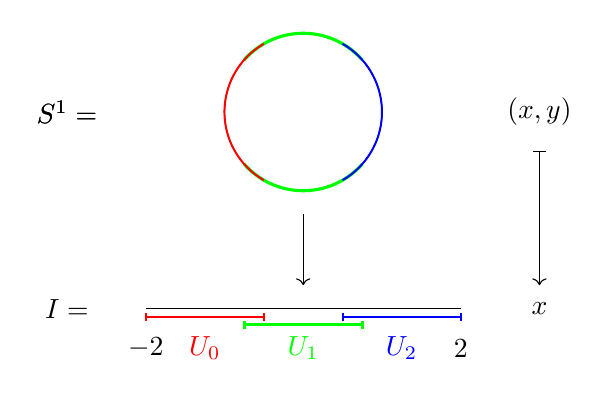
\begin{tikzpicture}
\draw (-2,0)--(2,0);
\draw (0,2.5) circle (1);
\draw[->] (0,1.2) -- (0,0.3);
\draw[|->] (3,2) -- (3,0.3);
\node () at (3,2.5) {$(x,y)$};
\node () at (3,0) {$x$};
\node () at (-3,2.5) {$S^1=$};
\node () at (-3,2.5) {$S^1=$};
\node () at (-3,0) {$I=$};
\node () at (-2,-0.5) {$-2$};
\node () at (2,-0.5) {$2$};
\draw[green,line width=0.4mm] (-3/4,-0.66143782776+2.5) arc (270-48.59:270+48.59:1);
\draw[green,line width=0.4mm] (3/4,0.66143782776+2.5) arc (90-48.59:90+48.59:1);
\draw[red,line width=0.25mm] (-1/2,2.5+0.866) arc (120:240:1);
\draw[blue,line width=0.25mm] (1/2,2.5+0.866) arc (60:-60:1);
\draw[red,line width=0.25mm] (-2,-0.1)--(-1/2,-0.1);
\draw[red,line width=0.25mm] (-2,-0.15)--(-2,-0.05);
\draw[red,line width=0.25mm] (-1/2,-0.15)--(-1/2,-0.05);
\draw[blue,line width=0.25mm] (2,-0.1)--(1/2,-0.1);
\draw[blue,line width=0.25mm] (2,-0.15)--(2,-0.05);
\draw[blue,line width=0.25mm] (1/2,-0.15)--(1/2,-0.05);
\draw[green,line width=0.4mm] (-3/4,-0.2)--(3/4,-0.2);
\draw[green,line width=0.4mm] (-3/4,-0.25)--(-3/4,-0.15);
\draw[green,line width=0.4mm] (3/4,-0.25)--(3/4,-0.15);
\node[red] () at (-5/4,-0.5) {$U_0$};
\node[green] () at (0,-0.5) {$U_1$};
\node[blue] () at (5/4,-0.5) {$U_2$};
\end{tikzpicture}
$$


Theorem: The spectral sequence of $K=\bigoplus K^{,q}$ applyed to $H^*(S^1)$, with $E^{p,q}_2 = \check{H}(\mathfrak{U},\mathcal{H}^q)$ , where $\mathcal{H}^q(U) = H^q(\pi^{-1}U)$.

The nerve is a linear graph:

$$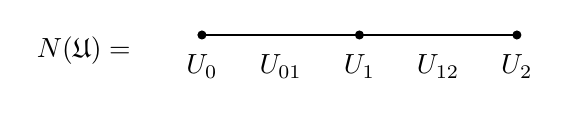
\begin{tikzpicture}
\node () at (-3.5,0.0) {$N(\mathfrak{U}) = $};
\draw (-2,0.2)--(2,0.2);
\node () at (-2,-0.2) {$U_0$};
\node () at (-1,-0.2) {$U_{01}$};
\node () at (0,-0.2) {$U_1$};
\node () at (1,-0.2) {$U_{12}$};
\node () at (2,-0.2) {$U_2$};
\draw[fill=black] (-2,0.2) circle (0.05);
\draw[fill=black] (0,0.2) circle (0.05);
\draw[fill=black] (2,0.2) circle (0.05);
\end{tikzpicture}
$$

We have
$$\mathcal{H}^q(U_0) = H^0(\pi^{-1}U_0) = \mathbb{R}$$
$$\mathcal{H}^q(U_1) = H^0(\pi^{-1}U_1) = \mathbb{R}^2$$
$$\mathcal{H}^q(U_2) = H^0(\pi^{-1}U_2) = \mathbb{R}$$
$$\mathcal{H}^q(U_{01}) = H^0(\pi^{-1}U_{01})=\mathbb{R}^2$$
$$\mathcal{H}^q(U_{12}) = H^0(\pi^{-1}U_{12})=\mathbb{R}^2$$

$$
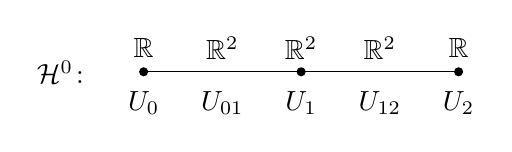
\begin{tikzpicture}
\node () at (-3,0.2) {$\mathcal{H}^0\colon$};
\draw (-2,0.2)--(2,0.2);
\node () at (-2,0.5) {$\mathbb{R}$};
\node () at (-1,0.5) {$\mathbb{R}^2$};
\node () at (0,0.5) {$\mathbb{R}^2$};
\node () at (1,0.5) {$\mathbb{R}^2$};
\node () at (2,0.5) {$\mathbb{R}$};
\draw (-2,0.2)--(2,0.2);
\node () at (-2,-0.2) {$U_0$};
\node () at (-1,-0.2) {$U_{01}$};
\node () at (0,-0.2) {$U_1$};
\node () at (1,-0.2) {$U_{12}$};
\node () at (2,-0.2) {$U_2$};
\draw[fill=black] (-2,0.2) circle (0.05);
\draw[fill=black] (0,0.2) circle (0.05);
\draw[fill=black] (2,0.2) circle (0.05);
\end{tikzpicture}
$$

We have

$E_1^{p,q} = H_d^{p,q}(K) = \prod H^q(\pi^{-1}U_{\alpha_0...\alpha_p})$

$$E_1 = \begin{array}{c|ccc}
q=1 & 0 & 0 & 0\\
q=0 & \mathbb{R}\oplus \mathbb{R}^2\oplus \mathbb{R} & \mathbb{R}^2\oplus \mathbb{R}^2 & 0\\
\hline
&p=0 & p=1 & p=2 \end{array}$$

where the only nonzero map $\delta\colon E_1^{0,0}\rightarrow E_1^{1,0}$ is (recall that $\delta$ is the alternating difference -- see Lecture 14)
$$\delta\colon (b,(c_1,c_2),d)\mapsto ((c_1-b,c_2-b),(d-c_1,d-c_2))$$

Then $\mathrm{ker}\delta = \{(b,(c_1,c_2)d)|b=c_1=c_2=d\} = \mathbb{R}$, so $E^{0,0}_2 = \mathrm{ker}\delta =  \mathbb{R}$, and $E^{1,0}_2 = \mathbb{R}^2\oplus \mathbb{R}^2/\mathrm{im}\delta = \mathbb{R}$. We have $E_2 = E_\infty = H^*(S^1)$, so we get
$$H^n(S^1) = \left\{\begin{array}{cc} \mathbb{R} & n=0,1\\0 & \text{otherwise}\end{array}\right..$$



\subsection{Lecture 28: Monodromy}

In Leray's spectral sequence for a map $\pi\colon Y\rightarrow X$, $E^{p,q}_2 = \check{H}^p(\mathfrak{U},\mathcal{H}^q)$, where $\mathcal{H}^q$ is the presheaf $\mathcal{H}^q(U) = H^q(\pi^{-1}U)$ on open cover $\mathfrak{U}$ of $X$.


Simplicial complexes: 

Def. A $p$-simplex spanned by $v_0,...,v_p$ in $\mathbb{R}^N$ in general positions (i.e. $v_1-v_0,...,v_p-v_0$ in $\mathbb{R}^N$ are linearly independent) is
$A:=\langle v_0,...,v_p\rangle = \{\sum_{i=0}^p t^iv_i | \sum t^i=1,t_i\geq 0\}$. 

Def. A face of $\langle v_0,...,v_p\rangle$ is a simplex spanned by a subset of $\{v_0,...,v_p\}$.

Def. A simplicial complex $K$ in $\mathbb{R}^N$ is a collection of simplices in $\mathbb{R}^N$, s.t. (i) every face of a simplex in $K$ is in $K$; (ii) intersection of any two simpliecs is a face of each of them. 

The edge groups of a simplicial complex $K$:

Def. An \emph{edge path} in $K$ is a sequence of vertices $v_0,v_1,...,v_k$ of vertices in which either $v_i=v_{i+1}$ or $v_iv_{i+1}$ is an edge. 

Def. An \emph{edge loop} is an edge path with $v_k=v_0$.

Def. The product of two edge paths $v_0...v_k$ and $v_k...v_l$ is a \emph{concatenation}:
$(v_0...v_k)\cdot (v_k...v_l) = v_0...v_kv_k...v_\ell$. (In order to achieve this, the end point of first path should equal the snitial point of the second path.)

Equivalence relation on edge paths:

(i) $...vv... \sim ...v...$
(ii) if $\langle u v \rangle$ is a 1-simplex, then $...uvu... \sim ...u...$ 
(iii) If $\langle uvw\rangle$ is a two simplex, then $...uvw...\sim ... uw...$

Example: $(v_0v_1v_2v_0)\cdot(v_0v_2v_1v_0) = \sim v_0$. 

Def. The \emph{edge group} $E(K,v_0)$ of a simplicial complex $K$ is the set of equivalence classes of edge loops at $v_0$ with concatination as product, $[v_0]$ as identity, and $[v_0v_1...v_{k-1}v_0]^{-1} = [v_0v_{k-1}...v_1v_0]$. 

Example: the triangle with three vertices and no faces, has  $E(K,v_0) = \mathbb{Z}$, generated by $[v_0v_1v_2v_0]$. 

Example: the triangle with three vertices and a filled face, has trivial group $E(K,v_0) = \{1\}$. 

The edge group does calculate the fundamental group of the topological space underlying the simplicial complex.

Locally constant and constant presheaves:

Def. A presheaf $\mathcal{F}$ on a topological space $X$ is \emph{constant with group $G$} if $\forall $ open set $U \in X$, $\mathcal{F}(U)=G$, and for $V\subset U\in \mathbf{Open}(X)$, the restriction $\mathcal{F}(U)\xrightarrow{\rho^U_V} \mathcal{F}(V)$ is the identity map $G\xrightarrow {id}G$. 


Let $\mathfrak{U}$ be an open cover of $X$. A \emph{presheaf} $\mathcal{F}$ on $U$ is \emph{constant with group G} is given by the same definition, but with $U\in \mathbf{Open}(\mathfrak{U}) := \{\text{nonempty finite intersections of open sets in }\mathfrak{U}\}$. 

Example: let $\mathcal{F}(U) = \{\text{locally constant function }f\colon U\rightarrow \mathbb{R}\}$ on topological space $X$. If $U = D\amalg D$, then $\mathcal{F}(U) = \mathbb{R}\oplus \mathbb{R}$. So $\mathcal{F}$ is not constant with group $\mathbb{R}$ on $X$. 

Suppose $\mathfrak{U}$ is a \emph{good cover} of $X$, i.e. all $U\in \mathbf{Open}(\mathfrak{U})$ are contractible.

Q: Is $\mathcal{F}$ constant with group $\mathbb{R}$ on $\mathfrak{U}$? A: Yes, it is $\underline{\mathbb{R}}$. 

Def. A presheaf $\mathcal{F}$ on a topological space $X$ is \emph{locally constant with group G} if $\forall$ $U\in \mathbf{U}(X)$, $\mathcal{F}(U) = G$ and $\forall$ $V\subset U\in \mathbf{U}(X)$, $\rho^U_V\colon \mathcal{F}(U)=G\rightarrow \mathcal{F}(V)=G$ is anisomorphism.


Example: locally constant presheaf that is not constant.

$$
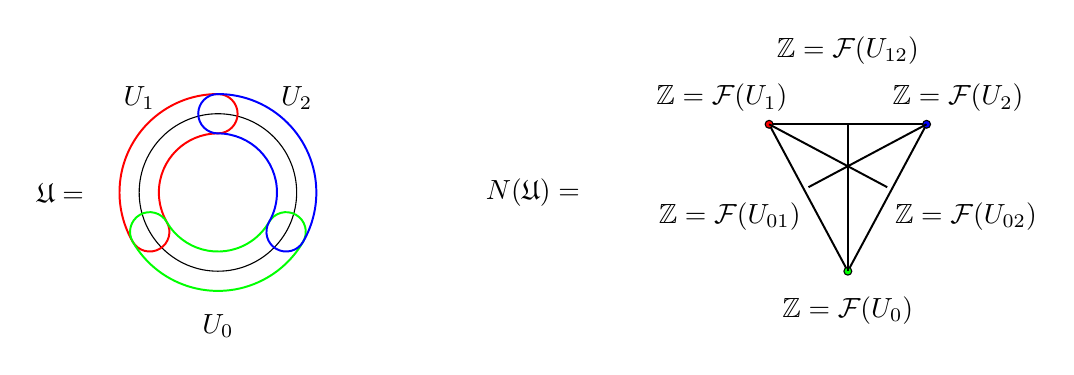
\begin{tikzpicture}
\node () at (-2,0.) {$\mathfrak{U}=$};
%\draw (-2,0.2)--(2,0.2);
\draw (0,0) circle (1);
%
\draw[red,line width=0.25mm] (0,0.75) arc (90:210:0.75);
\draw[red,line width=0.25mm] (0,1.25) arc (90:210:1.25);
\draw[red,line width=0.25mm] (0,1.25) arc (90:-90:0.25);
\draw[red,line width=0.25mm] (-1.0825317,-0.625) arc (210:390:0.25);
%
\draw[green,line width=0.25mm] (-1.0825317,-0.625) arc (210:330:1.25);
\draw[green,line width=0.25mm] (-0.649519,-0.375) arc (210:330:0.75);
\draw[green,line width=0.25mm] (1.0825317,-0.625) arc (-30:150:0.25);
\draw[green,line width=0.25mm] (-1.0825317,-0.625) arc (210:30:0.25);
%
\draw[blue,line width=0.25mm] (0,0.75) arc (90:-30:0.75);
\draw[blue,line width=0.25mm] (0,1.25) arc (90:-30:1.25);
\draw[blue,line width=0.25mm] (0,1.25) arc (90:270:0.25);
\draw[blue,line width=0.25mm] (1.0825317,-0.625) arc (330:150:0.25);
\node () at (4,0.) {$N(\mathfrak{U})=$};
\draw[line width=0.25mm] (-1+8,0.866)--(1+8,0.866);
\draw[line width=0.25mm] (-1+8,0.866)--(8,-1);
\draw[line width=0.25mm] (1+8,0.866)--(8,-1);
\draw[fill=blue] (1+8,0.866) circle (0.05);
\draw[fill=red] (-1+8,0.866) circle (0.05);
\draw[fill=green] (8,-1) circle (0.05);
\node () at (0,-1.7) {$U_0$};
\node () at (8,-1.5) {$\mathbb{Z}=\mathcal{F}(U_0)$};
\node () at (-1,1.2) {$U_1$};
\node () at (8-1.6,1.2) {$\mathbb{Z}=\mathcal{F}(U_1)$};
\node () at (1,1.2) {$U_2$};
\node () at (8+1.4,1.2) {$\mathbb{Z}=\mathcal{F}(U_2)$};
\node () at (8+1.5,-0.3) {$\mathbb{Z}=\mathcal{F}(U_{02})$};
\node () at (8,1.8) {$\mathbb{Z}=\mathcal{F}(U_{12})$};
\node () at (8-1.5,-0.3) {$\mathbb{Z}=\mathcal{F}(U_{01})$};

\draw[line width=0.25mm] (-1+8,0.866)--(8+1/2,0.067);
\draw[line width=0.25mm] (1+8,0.866)--(8-1/2,0.067);
\draw[line width=0.25mm] (8,0.866)--(8,-1);
\end{tikzpicture}
$$
Barycentric subdivision of $K$:
Def. The \emph{barycenter }of a $p$-simplex $A+ \langle v_0...v_p\rangle$ is $\hat{A} = \frac{1}{p+1} \sum_{i=0}^p v_i$ 

\begin{definition}[Barycentric subdivision] The \emph{barycentric subdivision} of a simplicial complex $K$ is the simplicial complex $K'$ obtained by $K$ by subdividing each simplex using its barycenter as a new vertex.
\end{definition}

Proposition: let $\mathfrak{U}$ be an open cover of topological space $X$, $N(\mathfrak{U})$ its nerve. then $\langle u_0...u_p\rangle \in N(\mathfrak{U})' \Leftrightarrow \exists$ permutation $\sigma \in S_{p+1}$ s.t. $U_{\sigma(0)}\subset U_{\sigma(1)}\subset \cdots \subset U_{\sigma(p)}$. 


A presheaf $\mathcal{F}$ on an open cover $\mathfrak{U}$ is an assignment of a group to each vertex of $N(\mathfrak{U})'$. 

If $\mathcal{F}$ is locally constant on $\mathfrak{U}$, and if $V\subset U$, then we can define $\rho^V_U:= (\rho^U_V)^{-1}$. Then a path $v_0v_1...v_k$ in $N(\mathfrak{U})'$ defines an isomorphism
$\mathcal{F}(V_0)\xrightarrow{\rho_{V_1}^{V_0}}\mathcal{F}(V_1)\xrightarrow{\rho_{V_2}^{V_1}}\mathcal{F}(V_2)
\rightarrow \cdots \rightarrow \mathcal{F}(V_l)$

So an edge loop of $N(\mathfrak{U})'$ at $U_0$ defines an automorphism of $\mathcal{H}(U_0)$. 

Theorem. Equivalent loops define the same automorphism of $\mathcal{F}(U_0)$. Thus, there is a map $E(N(\mathfrak{U})',U_0)\rightarrow \mathrm{Aut}(\mathcal{F}(U_0))$. So if $\mathcal{F}$ is locally constant on $\mathfrak{U}$, then this map is called the \emph{monodrony} of $\mathcal{F}$ on $\mathfrak{U}$.







\subsection{Lecture 29: When is a locally constant presheaf constant?}

Goal: $E^{p,q}_2 = \check{H}^p(\mathfrak{U},\mathcal{H}^q) = H^p(M)\otimes H^q(F)$ for a fiber bundle $\pi\colon E\rightarrow M$ with fiber $F$.

$X$: a topological space; $\mathfrak{U}$: an open cover of $X$; $N(\mathfrak{U})$: nerve of $\mathfrak{U}$; $N(\mathfrak{U})'$ the bary centric subdivision of $N(\mathfrak{U})$. 

A presheaf $\mathcal{F}$ on $\mathfrak{U}$ is a contravariant functor from $\mathbf{Open}(\mathfrak{U}) = \{\text{nonempty finite intersection of open sets in }\mathfrak{U}\}$ with morphisms the inclusions $=N(\mathfrak{U})'$, to the category of abelian groups.


$\mathcal{F}$ is \emph{locally constant} on $\mathfrak{U}$ with group $G$ if $\mathcal{F}(U_{\alpha_0...\alpha_0}) = G$ and $\rho^{v_\alpha}_{v_\beta}=$ isomorphisms.

$\mathcal{F}$ is \emph{constant} with group $G$ on $\mathfrak{U}$ if $\mathcal{F}(U_{\alpha_0...\alpha_0}) = G$ and $\rho^{v_\alpha}_{v_\beta} = 1$. 

Theorem. If $E(N(\mathfrak{U}',v_0)) = \{1\}$, then every locally constant presheaf on $\mathfrak{U}$ is isomorphic to a constant presheaf. 

Monodrony.

Lemma: if $v_0,v_1,v_2$ span a $2$-simplex in $N(\mathfrak{U})'$, then $\rho_0^1\rho_1^2 = \rho_0^2$. 

(use shorthand notation $\rho^i_j = \rho^{v_i}_{v_j}$).

(Proof omitted -- see youtube.)

So one can prove that $\rho^2_1\rho^0_2\rho^1_0=1$, and $\rho^1_0\rho^2_1\rho^0_2=1$.

Corollary. Going around a 2-simplex in $N(\mathfrak{U})'$ always gives 1. 

Theorem. Let $\mathcal{F}$ be a locally constant presheaf on an open $\mathfrak{U}$ of $X$. Equivalent edge paths from $v_0$ to $v_1$ in $N(\mathfrak{U})'$ induce the same isomorphism from $\mathcal{F}(v_0)$ to $\mathcal{F}(v_1)$. 

Proof: only need to check 3 basic equivalences introduced in the last lecture ($...vv...\sim ...v...$ which induces $...\rho^V_U\rho^V_V\rho^W_V...$ and $...\rho^V_U\rho^W_V...$; then $...WUVUZ...\sim ...WUZ...$, and then on the vertices of a 2-simplex, $...UVW...\sim ...UW...$m which amounts to $...\rho^V_U\rho^W_V...$ and $...\rho^W_U...$, which are equal by the previous lemma).

Corollary: Equivalent loops at $v_0$ in $N(\mathfrak{U})'$ induce the same automorphism of $\mathcal{F}(v_0)$. 

This gives map $\varphi\colon E(N(\mathfrak{U})',v_0)\rightarrow \mathrm{Aut}(\mathcal{F}(v_0))$, called the \emph{monodrony} of $\mathcal{F}$ on $\mathfrak{U}$. 

Theorem. Let $\mathfrak{U}$ be an open cover of a topological space $X$. If $N(\mathfrak{U})'$ is path connected and $E(N(\mathfrak{U})',v_0) = \{1\}$, then every locally constant presheaf $\mathcal{F}$ with group $G$ on $U$ is isomorphic to the constant presheaf with group $G$, denoted as $\underline{G}$.
	
(Proof -- see lecture video.)
	
Theorem: For $X$ path connected, $\pi_1(X,x_0)\simeq E(N(\mathfrak{U}),v_0)
\cong E(N(\mathfrak{U})',v_0)$.  (see the book, p148)
	
Now, apply the theorem to $E_2^{p,q}$:

Let $\pi\colon E\rightarrow M$ be a $C^\infty$ fiber bundle with fiber $F$. Let $\mathcal{H}^q(U) = H^q(\pi^{-1}U)$, a presheaf on $M$.

Proposition: $\mathcal{H}^q$ is locally constant on a good cover $\mathfrak{U}$ of $M$. 

(Assume $M$ is simply connected, then $E(N(\mathfrak{U})',v_0) = \{1\}$, so $\mathcal{H}^q$ is the constant presheaf with group $\mathcal{H}^q(U) = H^q(\pi^{-1}U) = H^q(U\times F) = H^q(F)$, $U\in N(\mathfrak{U})'$ is diffeomorphic to $\mathbb{R}^n$. So $\mathcal{H}^q\simeq \overline{H^q(F)} = \underline{\mathbb{R}\oplus \cdots \oplus\mathbb{R}}$ (assuming $H^q(F)$ finite dimensional).

Now, $E^{p,q}_2 = \check{H}(\mathfrak{U},\mathcal{H}^q) = \check{H}(\mathfrak{U},\overline{\mathbb{R}\oplus \cdots \oplus \mathbb{R}}) = \check{H}(\mathfrak{U},\overline{\mathbb{R}})\oplus \cdots \oplus 
\check{H}(\mathfrak{U},\overline{\mathbb{R}})\simeq H^p(M)\oplus \cdots \oplus H^p(M)
=H^p(m)\otimes (\mathbb{R}\oplus \cdots \oplus \mathbb{R}) = H^p(M)\otimes H^q(F)$, under two hypothesis: (1) $M$ is simply connected and (2) $H^*(F)$ is finite dimensional.










	

\end{document}
